\label{chpt:characterisation of 12 new CVs} % for referencing this chapter elsewhere, use \ref{chpt:label}
\lhead{\emph{Eclipse modelling of 12 CVs}} % This is for the header on each page - perhaps a shortened title

A modest backlog of observed CV eclipse light curve data was reduced, calibrated, and modelled following the procedure outlined in \S\ref{sect:modelling:eclipse modelling}, and the results are presented here.

The systems modelled in this chapter were chosen largely based on their short periods, targeting the donor mass range for which mass loss rates could be inferred ($0.08 M_\odot < M_{\rm donor} < 0.20 M_\odot$, shown in \S\ref{sect:results:MESA massloss allowable mass range}). They range in period from $1.4 - 2.2$ hours, and were drawn from a few sources.
The All-Sky Automated Survey for Supernovae (ASASSN) \citep{shappee2014} is sensitive to transients, and is a valuable tool to identify CVs by their outbursts for follow-up once they re-enter quiescence; such systems are recognised by their ASASSN moniker.
Other candidate systems were gathered from a variety of sources, which are cited below.
% The vsnet alert system also provided several systems, which are marked below with (v).
The modelled systems in this thesis were:
\begin{itemize}
    \setlength\itemsep{0em}
    \item ASASSN-14hq
    \item ASASSN-14kb (a.k.a OGLE-LMC529.30.114)
    \item ASASSN-15pb
    \item ASASSN-17fo
    \item AY For (a.k.a H$\alpha$0242-2802) \citep{woudt2004}
    \item CSS090622 J215636+193242 (hereafter CSS090622) \citep{kato2012,thorstensen2016}
    \item CSS090102 J132536+210037 (hereafter CSS090102) \citep{kato2012}
    \item CSS090419 J162620-125557 (hereafter CSS090419) \citep{kato2012}
    \item MASTER OT J001400.25-561735.0 (hereafter MAS0014) (Woudt, private communication)
    \item OGLE BLG-ECL-000082 (a.k.a BLG510.16.126296, hereafter OGLE82) \citep{soszynski2016}
    \item SDSS J074859.6+312512.7 (hereafter SDSS J0748) \citep{kato2016}
    \item SDSS J152419.33+220920.0 (hereafter SDSS J1524) \citep{southworth2010,michel2013}
\end{itemize}
\newpage
ASASSN-14hq and ASASSN-15pb were observed by \citet{paterson2019} and had their periods measured, though the observations used in this thesis pre-date this publication and I make my own independent measurement of the period.
These two systems were also noted to be in outburst in late 2014 in the case of ASASSN-14hq, and 2015 in the case of ASASSN-15pb.
Table~\ref{table:three white dwarfs:observational data} summarises the right ascension, declination, magnitude, and ephemeris of the CVs observed here.

\newpage
% \begin{landscape}
    \begin{table}
        \begin{adjustwidth}{-.5in}{-.5in}
            \centering
            \captionsetup{justification=centering}
            \caption{Summary of observational information for the 12 CVs of this chapter. }
            \begin{tabular}{lccccc}
                \hline
                {\bf System name} & {\bf RA} & {\bf Dec} & {\bf $g'$}      & {\bf $T_0$,}    & {\bf Period,} \\
                                  &          &           &                 & {\bf BMJD, UTC} & {\bf days}      \\
                \hline
                \hline
                ASASSN-14hq     & 06:38:19.59 & -48:59:16.1 & 18.1 & 57701.27140(2) & 0.074326999(3) \\
                ASASSN-14kb     & 04:46:50.01 & -71:22:56.0 & 18.6 & 58143.16048(2) & 0.0681057(4) \\
                ASASSN-15pb     & 20:14:22.92 & -63:37:58.6 & 19.5 & 57626.14278(3) & 0.093290(6) \\
                ASASSN-17fo     & 11:38:35.70 & +04:44:54.5 & 19.6 & 58143.24296(2) & 0.061548(1) \\
                AY For          & 02:42:34.82 & -28:02:44.0 & 18.2 & 57701.10964(1) & 0.07461485(4) \\
                CSS090102       & 13:25:36.06 & +21:00:36.8 & 19.8 & 55943.12147(2) & 0.062384910(2) \\
                CSS090419       & 16:26:19.83 & -12:55:56.5 & 20.5 & 56498.92855(3) & 0.075442759(3) \\
                CSS090622       & 21:56:36.34 & +19:32:41.5 & 19.3 & 56874.20195(4) & 0.0709293(7) \\
                MAS0014         & 00:14:00.25 & -56:17:35.0 & 18.3 & 57626.08355(1) & 0.07152949(1) \\
                OGLE82          & 17:54:16.19 & -35:26:39.5 & 18.0 & 57623.03460(2) & 0.071930828(3) \\
                SDSS J0748      & 07:48:59.56 & +31:25:12.7 & 17.8 & 57808.63030(1) & 0.058311083(3) \\
                SDSS J1524      & 15:24:19.33 & +22:09:20.1 & 19.1 & 56486.91456(1) & 0.065318733(1) \\
                \hline
            \end{tabular}
        \end{adjustwidth}
    \end{table}
% \end{landscape}


\section{Results}
\label{sect:results:12 new CVs:results}

All eclipses presented are well-described by their fits, with small residuals. The light curves are shown below, along with the white dwarf flux distributions their best-fit white dwarf model atmospheres, and notes on the modelling of each system.
Table~\ref{table:12 new cvs:system_parameters} details the physical parameters of these 12 new systems.

In a few cases, the GP appears as a flat line along a residual of 0 despite some obvious scatter, e.g. ASASSN-14hq, seen in Figure~\ref{fig:ASASSN-14hq all light curves cont}. This is expected, as in these cases the residuals are fully described by the error in flux and the GP likelihood becomes dominated by the priors, sampling small values of GP amplitude.

None of these systems presented the issues with their characterisations that was seen in Chapter~\ref{chpt:three peculiar white dwarfs}. The modelled white dwarf colours were described by cooling tracks well in most cases, with the exceptions of CSS090419 and CSS090622. Spectroscopic follow-up in these cases is desirable to probe these systems more deeply.

Some results are particularly good demonstrations of the ability of the hierarchical GP modelling approach to usefully model poorer quality light curves in tandem with higher quality data.
An example of this is seen in the case of MAS0014, the light curves of which are seen in Figures~\ref{fig:MAS0014 all light curves},~\ref{fig:MAS0014 all light curves cont 1},~and~\ref{fig:MAS0014 all light curves cont 2}, where the high-quality binned data help a subtle bright spot egress to be confidently constrained in the eclipse of 2016/11/07 even in the presence of significant flickering.
A more extreme example is that of SDSS J0748, which has the white dwarf and bright spot ingresses blended together for the majority of observations, but clearly distinct ingresses on the night of 2018/02/05 and somewhat distinct ingresses on 2018/02/07, seen in Figure~\ref{fig:SDSS J0748 all light curves}.
Using the hierarchical structure to share information between observations constrains the parameter space, and makes characterisation possible in a system that would otherwise be extremely difficult to model.

When optimising the eclipse model to the data, some systems had their eclipses binned together where appropriate to reduce the complexity of the parameter space, and the observing logs in \S\ref{sect:observing:observation catalogue} details which eclipses were combined. However, in the interests of readability, the dates of the data that are binned for a given light curve are also noted in the figure caption. For unbinned data, the date and approximate mid-eclipse time is given in the axis title.
The majority of observations were made with ULTRACAM, though some systems are supported by ULTRASPEC data.



\newpage
\subsection{ASASSN-14hq}

The period of this system was measured by \citet{paterson2019} to be $0.074327(9)$ days, consistent with my own measurement of $0.074326999(3)$ days.
These observations fell into two binning categories: the 2016 and 2017 data, and the January 2018 data -- specific observation logs are given in Table~\ref{table:observing:observation logs ASASSN-14hq}.
Eclipse modelling indicates that the disc radius fell in brightness by $\sim 20\%$ in the $g'$ and $\sim 50\%$ in the $u'$ between these two batches, suggesting the disc may have been in a phase of dumping material onto the white dwarf faster than material enters it from the donor during this period. As this system was observed in outburst only two years prior to these observations, this is not unexpected.

For this system, the white dwarf fluxes were well-described by the model cooling tracks, with the white dwarf fitting phase producing a value of $\pi$ that agrees with Gaia ($3.40\pm0.07$ mas and $3.40\pm0.08$ mas, respectively).
Fitting found a somewhat low mass white dwarf, $0.67 \pm 0.07 M_\odot$, though this falls just over $1\sigma$ outside the intrinsic scatter of the \citet{pala2020} population measurement of $0.83\pm0.13 M_\odot$ so is well within the expected range. Models converged on a donor mass of $0.097\pm0.002 M_\odot$, consistent with the pre-period minimum CV track that amplifies gravitational braking by a factor of $\sim 2.5$.


% \begin{landscape}
%     \begin{table}
	\begin{center}
		\caption{Observations taken for ASASSN-14hq. Mid-eclipse times and cycle numbers are calculated following the method detailed in \S\ref{sect:modelling:getting ephemeris}.}
		\label{table:observing:observation logs ASASSN-14hq}
		\begin{tabular}{ccccccccc}
			\hline
			Instrument & Telescope & Date & Observation  & Observation  & Filter(s) & $T_{\rm ecl}$ & Cycle No. & Binning \\
			 &  &  &  start &  end &  &  &  & ID \\
			 &  &  & TDB & TDB &  & MJD &  &  \\
			\hline
			\hline
			 UCAM & NTT & 2016/11/9  & 06:06 & 06:45 & $u_{\rm reg},g_{\rm reg},r_{\rm reg}$ & 57701.27137(1) &    0 & A \\
			 UCAM & NTT & 2016/11/11 & 06:22 & 06:49 & $u_{\rm reg},g_{\rm reg},r_{\rm reg}$ & 57703.27826(1) &   27 & A \\
			 UCAM & NTT & 2017/3/19  & 02:25 & 03:09 & $u_{\rm reg},g_{\rm reg},r_{\rm reg}$ & 57831.12065(1) & 1747 & A \\
			 UCAM & NTT & 2017/3/21  & 23:59 & 00:44 & $u_{\rm reg},g_{\rm reg},r_{\rm reg}$ & 57834.01942(1) & 1786 & A \\
			 UCAM & NTT & 2018/1/23  & 00:55 & 01:48 & $u_{\rm sup},g_{\rm sup},r_{\rm sup}$ & 58141.06425(1) & 5917 & B \\
			 UCAM & NTT & 2018/1/25  & 01:19 & 01:57 & $u_{\rm sup},g_{\rm sup},r_{\rm sup}$ & 58143.07107(2) & 5944 & B \\
			 UCAM & NTT & 2018/1/28  & 02:28 & 03:05 & $u_{\rm sup},g_{\rm sup},r_{\rm sup}$ & 58146.11846(2) & 5985 & B \\
			 UCAM & NTT & 2018/1/28  & 04:09 & 04:49 & $u_{\rm sup},g_{\rm sup},r_{\rm sup}$ & 58146.19283(2) & 5986 & B \\
			 UCAM & NTT & 2018/1/30  & 01:04 & 01:29 & $u_{\rm sup},g_{\rm sup},r_{\rm sup}$ & 58148.05102(3) & 6011 & B \\
			\hline
			\end{tabular}
	\end{center}
\end{table}
% \end{landscape}

\begin{figure}
    \centering
    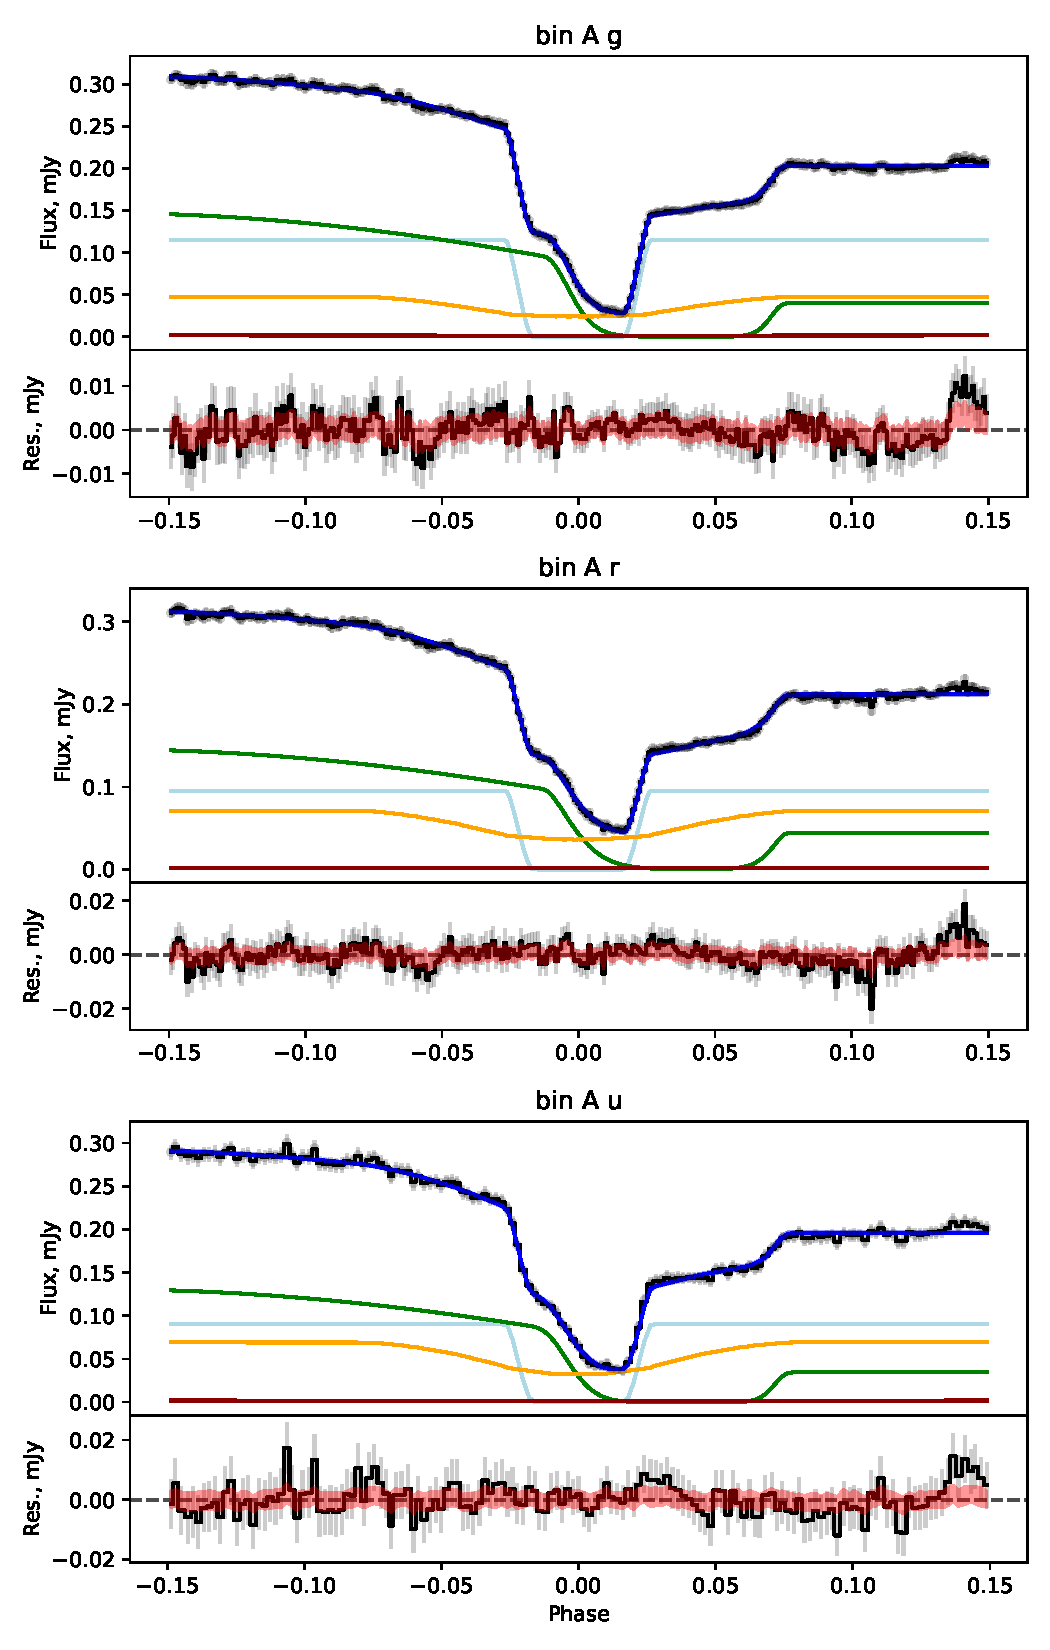
\includegraphics[width=\textwidth]{figures/results/ASASSN-14hq/ASASSN-14hq_1.pdf}
    \caption{ASASSN-14hq light curve models. Symbols are the same as Figure~\ref{fig:ASASSN-17jf all light curves}. Data are the result of binning the following nights: 2016/11/9, 2016/11/11, 2017/3/19, 2017/3/21.}
    \label{fig:ASASSN-14hq all light curves}
\end{figure}
\begin{figure}
    \centering
    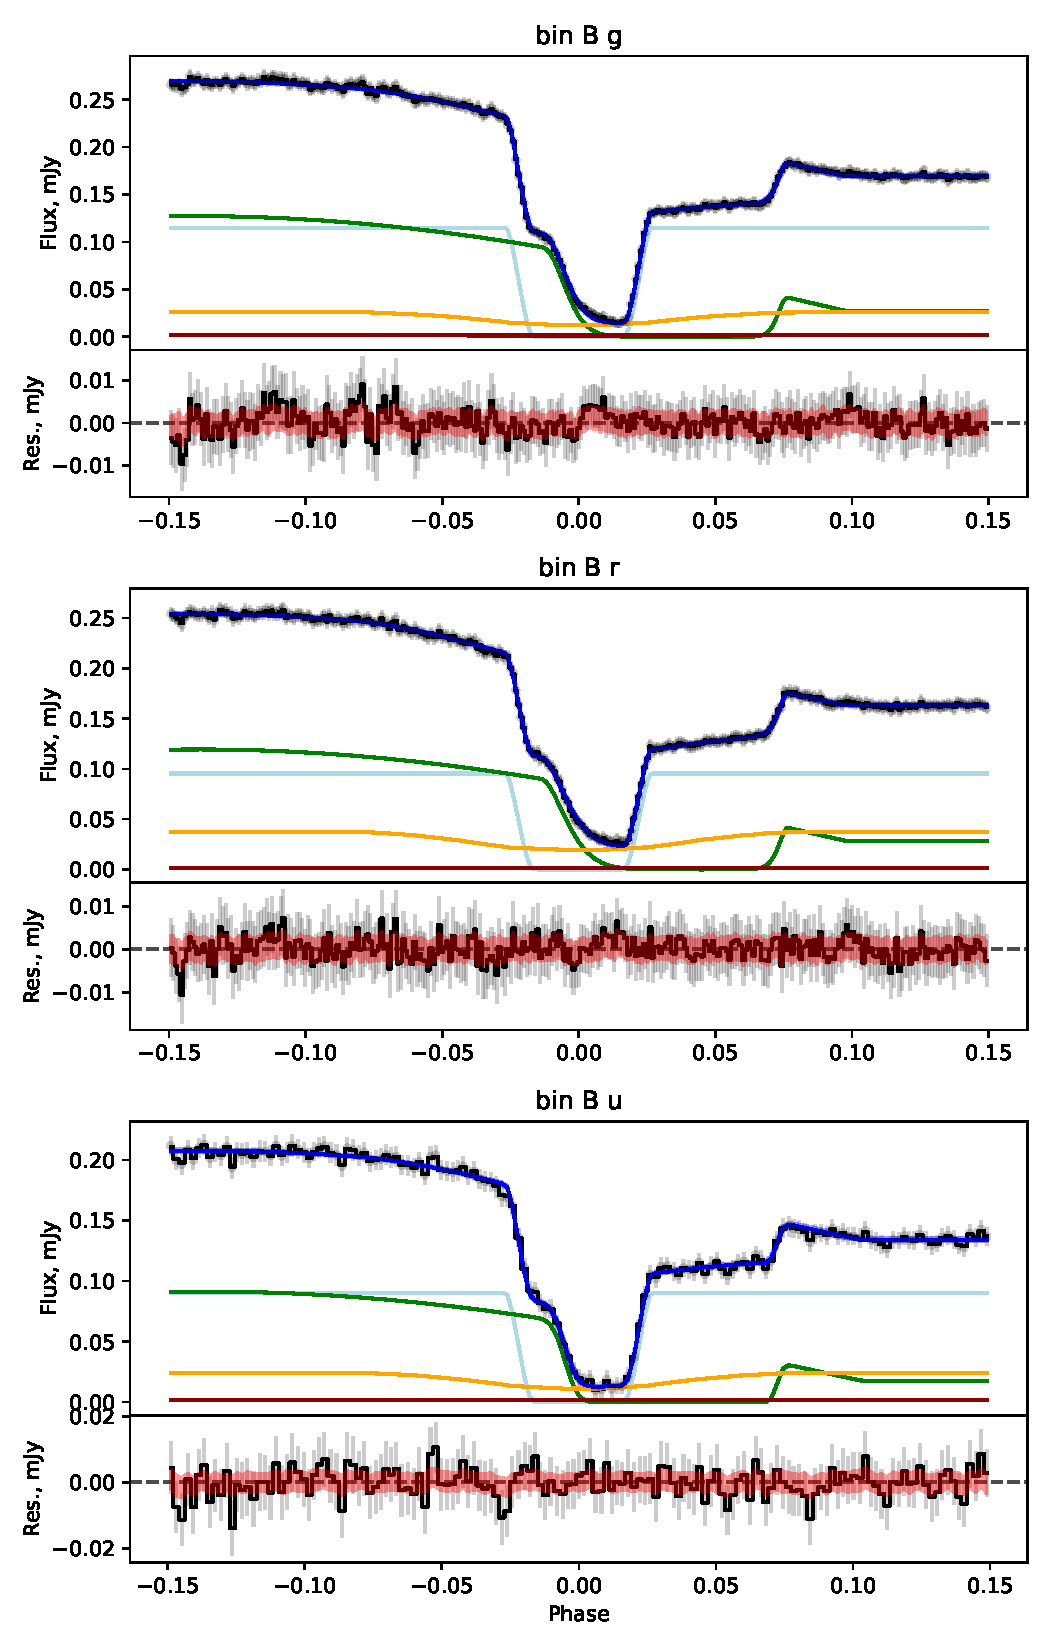
\includegraphics[width=\textwidth]{figures/results/ASASSN-14hq/ASASSN-14hq_2.pdf}
    \caption{ASASSN-14hq light curve models (cont.). Data are the result of binning the following nights: 2018/1/23, 2018/1/25, both 2018/1/28 observations, 2018/1/30.}
    \label{fig:ASASSN-14hq all light curves cont}
\end{figure}
\begin{figure}
    \centering
    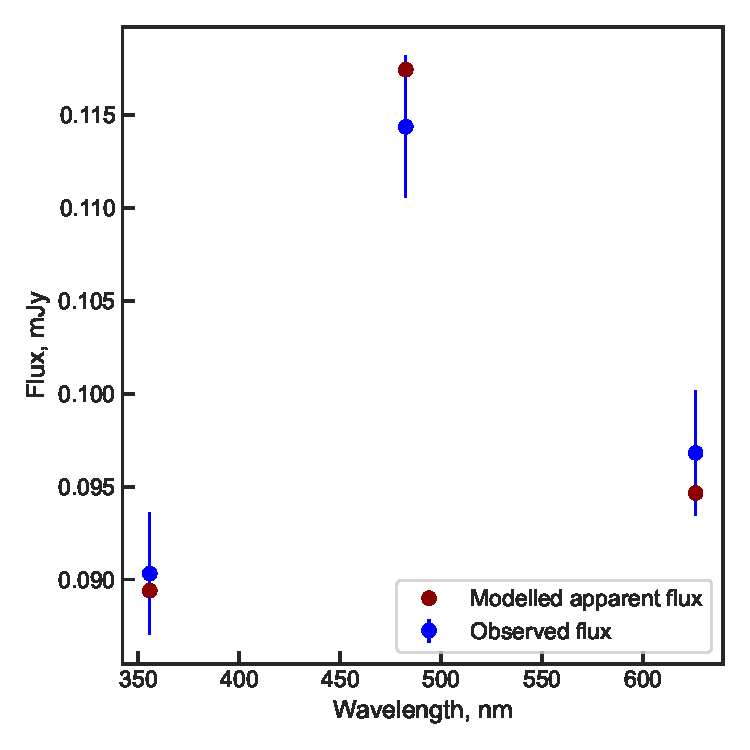
\includegraphics[width=\textwidth]{figures/results/ASASSN-14hq/fluxplot.pdf}
    \caption{ASASSN-14hq observed white dwarf fluxes, compared to the best-fit model atmosphere.}
    \label{fig:ASASSN-14hq flux plot}
\end{figure}
\clearpage



\newpage
\subsection{ASASSN-14kb}

ASASSN-14kb has very distinct modelling features, making it an easily characterised system. The 4 observations showed little variance between them, and the binned light curves seen in Figure~\ref{fig:ASASSN-14kb all light curves} show remarkably little residual flickering. Additionally, the white dwarf spectral energy distribution was well-described by the cooling tracks and exactly reproduces the Gaia $\pi$ distribution of $2.78\pm0.11$.
The resulting donor mass of this CV appears to be significantly high for the observed period, sitting $\sim 3\sigma$ above the purely gravitational wave driven MESA donor track.

% \begin{landscape}
%     \begin{table}
	\begin{center}
		\begin{tabular}{cccccccc}
			\hline
			Instrument & Telescope & Date & Observation start & Observation end & Filter(s) & $T_{\rm ecl}$ & Cycle No. \\
			 &  &  & UTC & UTC &  & BMJD &  \\
			\hline
			\hline
			UCAM & NTT & 2018/1/20 & 01:01 & 01:32 & $u_{\rm sup},g_{\rm sup},r_{\rm sup}$ & 58138.05257(1)                                                                                                            &                                         -75 \\
			UCAM & NTT & 2018/1/23 & 05:25 & 06:24 & $u_{\rm sup},g_{\rm sup},r_{\rm sup}$ & 58141.25354(1)                                                                                                            &                                         -28 \\
			UCAM & NTT & 2018/1/25 & 03:12 & 04:11 & $u_{\rm sup},g_{\rm sup},r_{\rm sup}$ & 58143.16050(1)                                                                                                            &                                           0 \\
			UCAM & NTT & 2018/1/26 & 02:06 & 02:56 & $u_{\rm sup},g_{\rm sup},r_{\rm sup}$ & 58144.11398(2)                                                                                                            &                                          14 \\
		   \hline
		\end{tabular}
	\end{center}
	\caption{Observations taken for ASASSN-14kb.}
	\label{table:observing:observation logs ASASSN-14kb}
\end{table}
% \end{landscape}

\begin{figure}
    \centering
    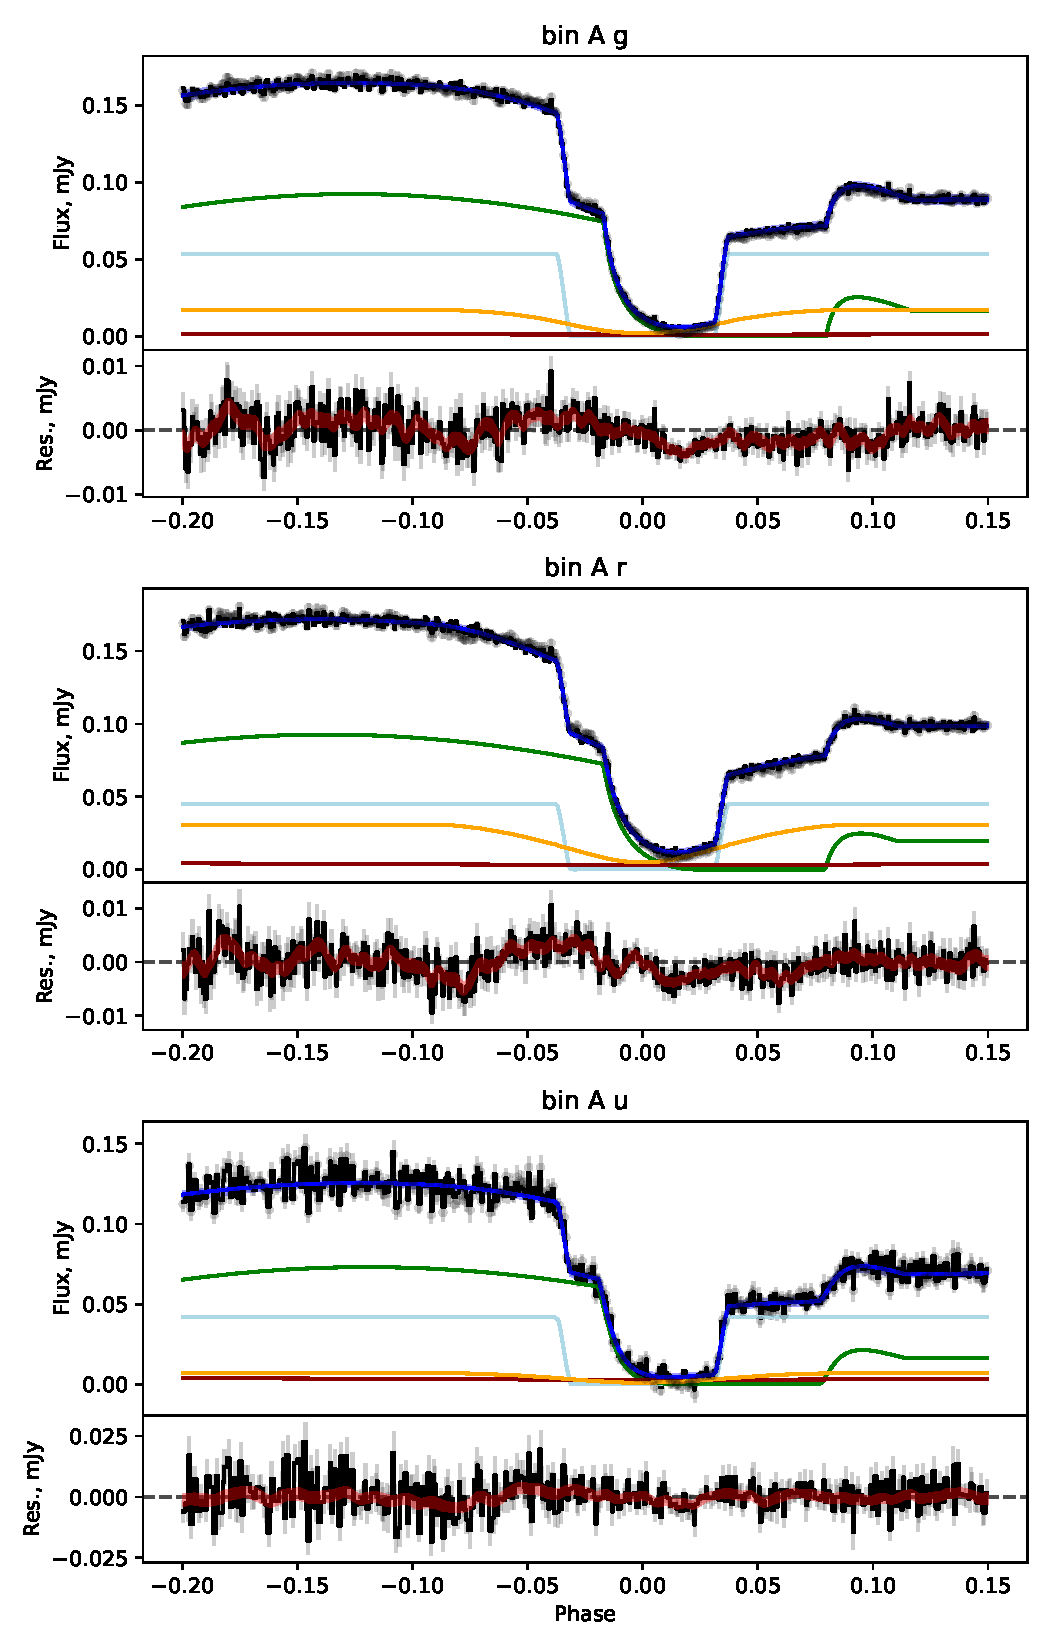
\includegraphics[width=\textwidth]{figures/results/ASASSN-14kb/ASASSN-14kb_1.pdf}
    \caption{ASASSN-14kb light curve models. Symbols are the same as Figure~\ref{fig:ASASSN-17jf all light curves}}
    \label{fig:ASASSN-14kb all light curves}
\end{figure}
\begin{figure}
    \centering
    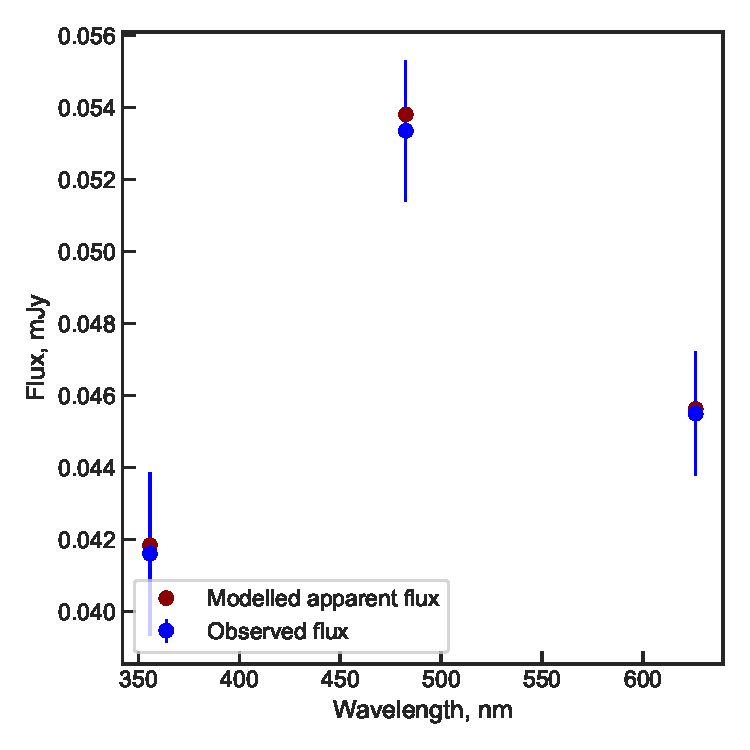
\includegraphics[width=\textwidth]{figures/results/ASASSN-14kb/fluxplot.pdf}
    \caption{ASASSN-14kb observed white dwarf fluxes, compared to the best-fit model atmosphere.}
    \label{fig:ASASSN-14kb flux plot}
\end{figure}
\clearpage



\newpage
\subsection{ASASSN-15pb}

ASASSN-15pb was an ideal candidate for modelling. The data in all bands were consistent enough to be comfortably binned together, aided by the 6 observations spanning only 6 days.
The observations of this system take place in August 2016, only a year after the system was observed in outburst, but the system appears to have quickly returned to a reasonably well-behaved state and is suitable for modelling.
The bright spot and white dwarf ingresses are mildly blended in the $u'$, $g'$, and $r'$ observations, and slightly more strongly blended in the $i'$ band. Whilst this did not prevent the optimisation from strongly constraining the white dwarf fluxes (with the exception of the loosely constrained $i'$ band flux), this blending makes constraining the eclipse width, $\Delta\phi$, and white dwarf radius more challenging. Despite this, by drawing on information from all eclipses the quantities are well-constrained, and the white dwarf fluxes are well-described by the model cooling tracks, so the resulting system parameters cab be considered sound.

\citet{paterson2019} measure the period of this system to be $0.09329(2)$ days, which is consistent with my measurement of $0.093290(6)$ days.
This is the longest period CV in this new sample, lying in the region defined as the period gap by the \citet{knigge11} donor tracks. However, the donor mass is significantly lower than the $0.20 M_\odot$ period gap mass assumed by \citet{knigge11}, at $0.148\pm0.008 M_\odot$.

% \begin{landscape}
%     \begin{table}
	\begin{center}
		\caption{Observations taken for ASASSN-15pb.}
		\label{table:observing:observation logs ASASSN-15pb}
		\begin{tabular}{ccccccccc}
			\hline
			Instrument & Telescope & Date & Observation  & Observation  & Filter(s) & $T_{\rm ecl}$ & Cycle No. & Binning \\
			 &  &  &  start &  end &  &  &  & ID \\
			 &  &  & TDB & TDB &  & MJD &  &  \\
			\hline
			\hline
			UCAM & NTT & 2016/8/20 & 23:33 & 00:37 & $u_{\rm reg},g_{\rm reg},r_{\rm reg}$ & 57621.01182(3) & -55 & A \\
			UCAM & NTT & 2016/8/22 & 02:37 & 03:25 & $u_{\rm reg},g_{\rm reg},r_{\rm reg}$ & 57622.13130(5) & -43 & A \\
			UCAM & NTT & 2016/8/22 & 04:39 & 05:39 & $u_{\rm reg},g_{\rm reg},r_{\rm reg}$ & 57622.22458(4) & -42 & A \\
			UCAM & NTT & 2016/8/23 & 01:02 & 01:50 & $u_{\rm reg},g_{\rm reg},r_{\rm reg}$ & 57623.06421(2) & -33 & A \\
			UCAM & NTT & 2016/8/25 & 04:44 & 05:19 & $u_{\rm reg},g_{\rm reg},r_{\rm reg}$ & 57625.20988(2) & -10 & A \\
			UCAM & NTT & 2016/8/26 & 02:56 & 03:39 & $u_{\rm reg},g_{\rm reg},r_{\rm reg}$ & 57626.14278(2) &   0 & A \\
		   \hline
		\end{tabular}
	\end{center}
\end{table}
% \end{landscape}

\begin{figure}
    \centering
    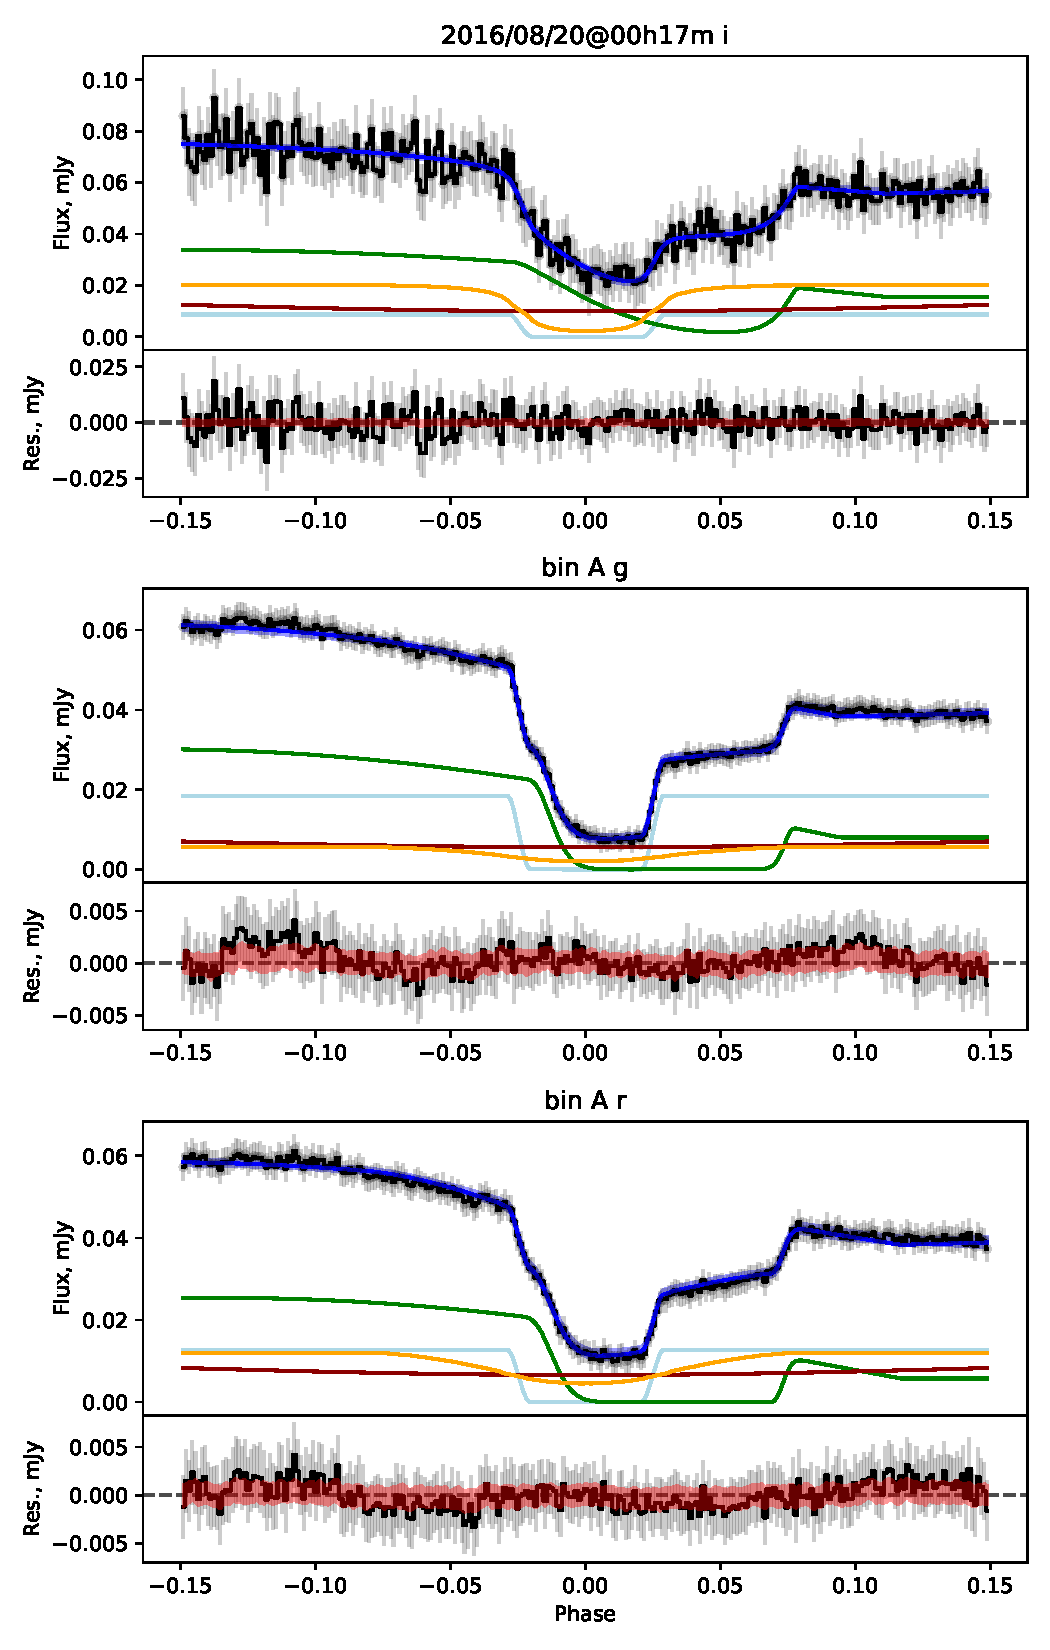
\includegraphics[width=\textwidth]{figures/results/ASASSN-15pb/ASASSN-15pb_1.pdf}
    \caption{ASASSN-15pb light curve models. Symbols are the same as Figure~\ref{fig:ASASSN-17jf all light curves}. $u'$, $g'$, and $r'$ data are the result of binning together all observations.}
    \label{fig:ASASSN-15pb all light curves}
\end{figure}
\begin{figure}
    \centering
    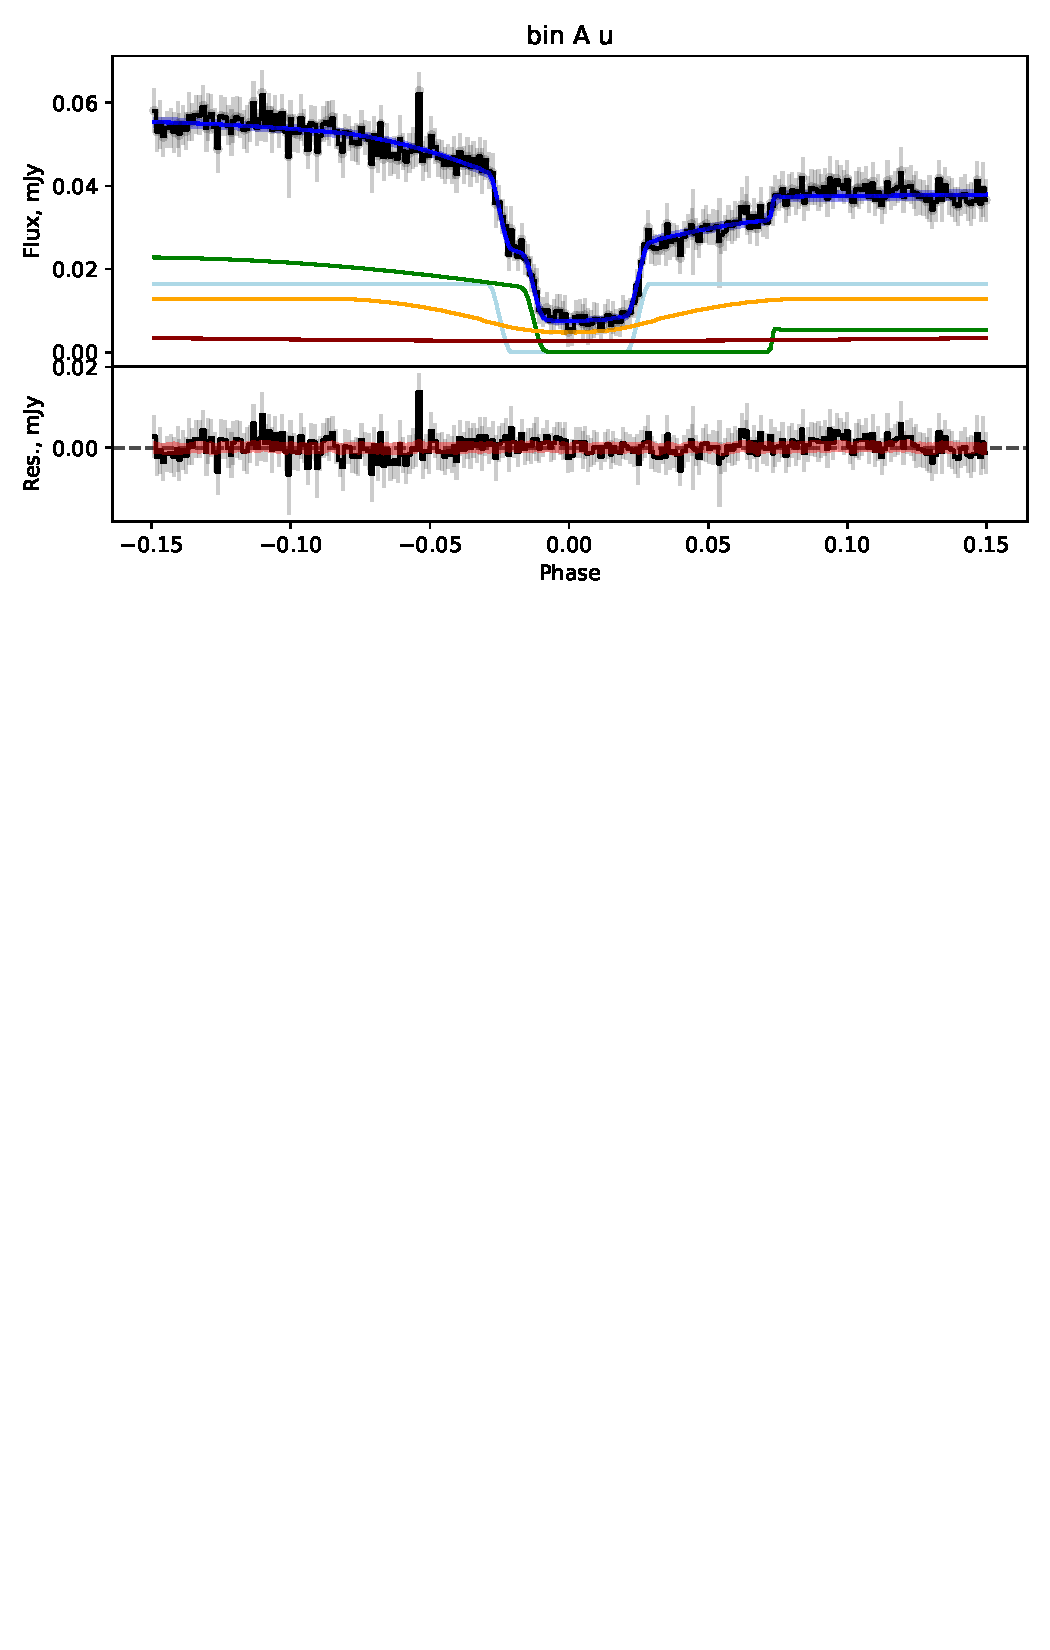
\includegraphics[width=\textwidth, trim={0cm 17cm 0cm 0cm}, clip]{figures/results/ASASSN-15pb/ASASSN-15pb_2.pdf}
    \caption{ASASSN-15pb light curve models (cont.)}
    \label{fig:ASASSN-15pb all light curves cont 1}
\end{figure}
\begin{figure}
    \centering
    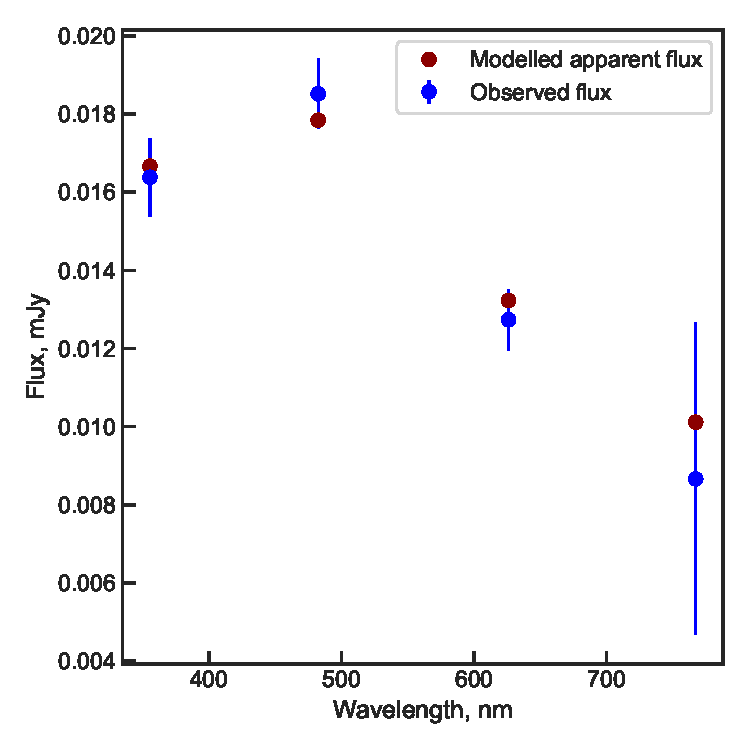
\includegraphics[width=\textwidth]{figures/results/ASASSN-15pb/fluxplot.pdf}
    \caption{ASASSN-15pb observed white dwarf fluxes, compared to the best-fit model atmosphere.}
    \label{fig:ASASSN-15pb flux plot}
\end{figure}
\clearpage


\newpage
\subsection{ASASSN-17fo}

ASASSN-17fo was observed in early 2018, and whilst the three eclipses were not suitably concordant to allow them to be binned together, the relevant eclipse features for modelling are impressively distinct with little flickering present. The resulting eclipse model described the data well, and the white dwarf fluxes find a good solution to models with $M_\mathrm{wd} = 0.85\pm0.01 M_\odot$ and a parallax of $1.79\pm0.20$~mas, in strong agreement with the Gaia $\pi$ of $1.96 \pm 0.20$~mas. However, the donor mass and period place this system well above the `standard' \citet{knigge11} donor track in Figure~\ref{fig:12 new cvs:donor model with eclipsers plotted}.


% \begin{landscape}
%     \begin{table}
	\begin{center}
		\caption{Observations taken for ASASSN-17fo.}
		\label{table:observing:observation logs ASASSN-17fo}
		\begin{tabular}{ccccccccc}
			\hline
			Instrument & Telescope & Date & Observation  & Observation  & Filter(s) & $T_{\rm ecl}$ & Cycle No. & Binning \\
			 &  &  &  start &  end &  &  &  & ID \\
			 &  &  & TDB & TDB &  & MJD &  &  \\
			\hline
			\hline
			UCAM & NTT & 2018/1/24 & 05:55 & 06:19 & $u_{\rm sup},g_{\rm sup},r_{\rm sup}$ & 58142.25819(1) & -16 & - \\
			UCAM & NTT & 2018/1/25 & 05:10 & 05:55 & $u_{\rm sup},g_{\rm sup},r_{\rm sup}$ & 58143.24296(1) &   0 & - \\
			UCAM & NTT & 2018/1/26 & 06:34 & 07:03 & $u_{\rm sup},g_{\rm sup},r_{\rm sup}$ & 58144.28927(2) &  17 & - \\
		   \hline
		\end{tabular}
	\end{center}
\end{table}
% \end{landscape}

\begin{figure}
    \centering
    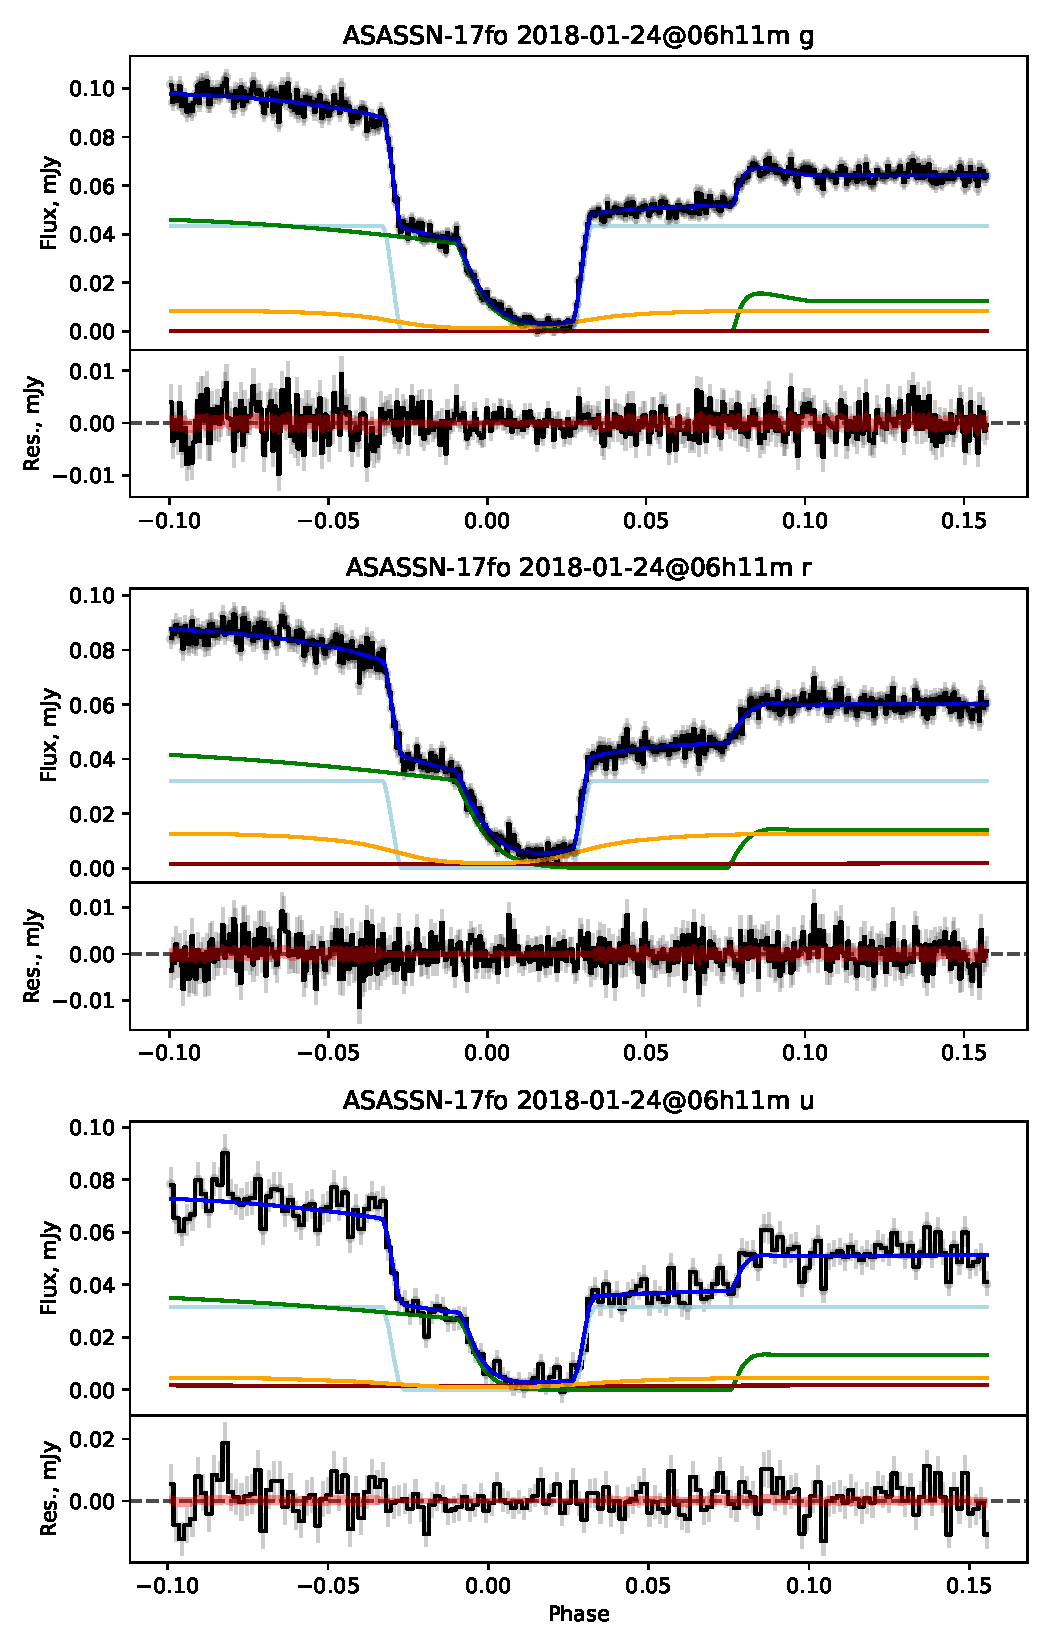
\includegraphics[width=\textwidth]{figures/results/ASASSN-17fo/ASASSN-17fo_1.pdf}
    \caption{ASASSN-17fo light curve models. Symbols are the same as Figure~\ref{fig:ASASSN-17jf all light curves}}
    \label{fig:ASASSN-17fo all light curves}
\end{figure}
\begin{figure}
    \centering
    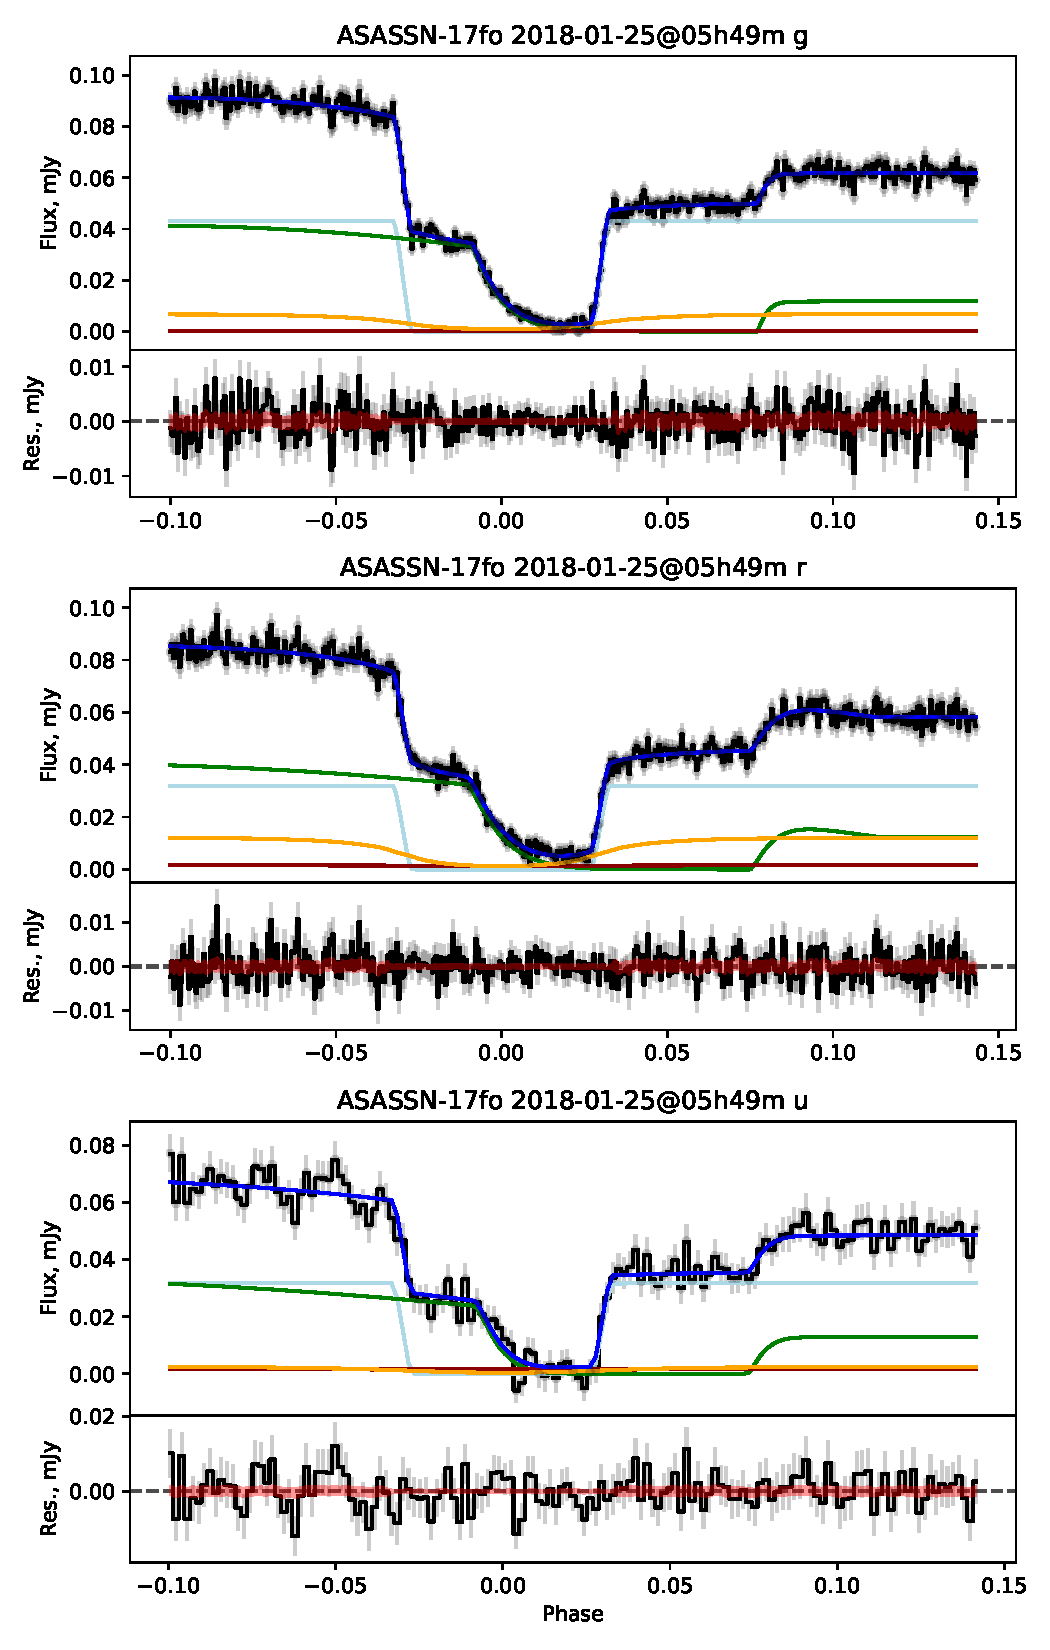
\includegraphics[width=\textwidth]{figures/results/ASASSN-17fo/ASASSN-17fo_2.pdf}
    \caption{ASASSN-17fo light curve models (cont.)}
    \label{fig:ASASSN-17fo all light curves cont 1}
\end{figure}
\begin{figure}
    \centering
    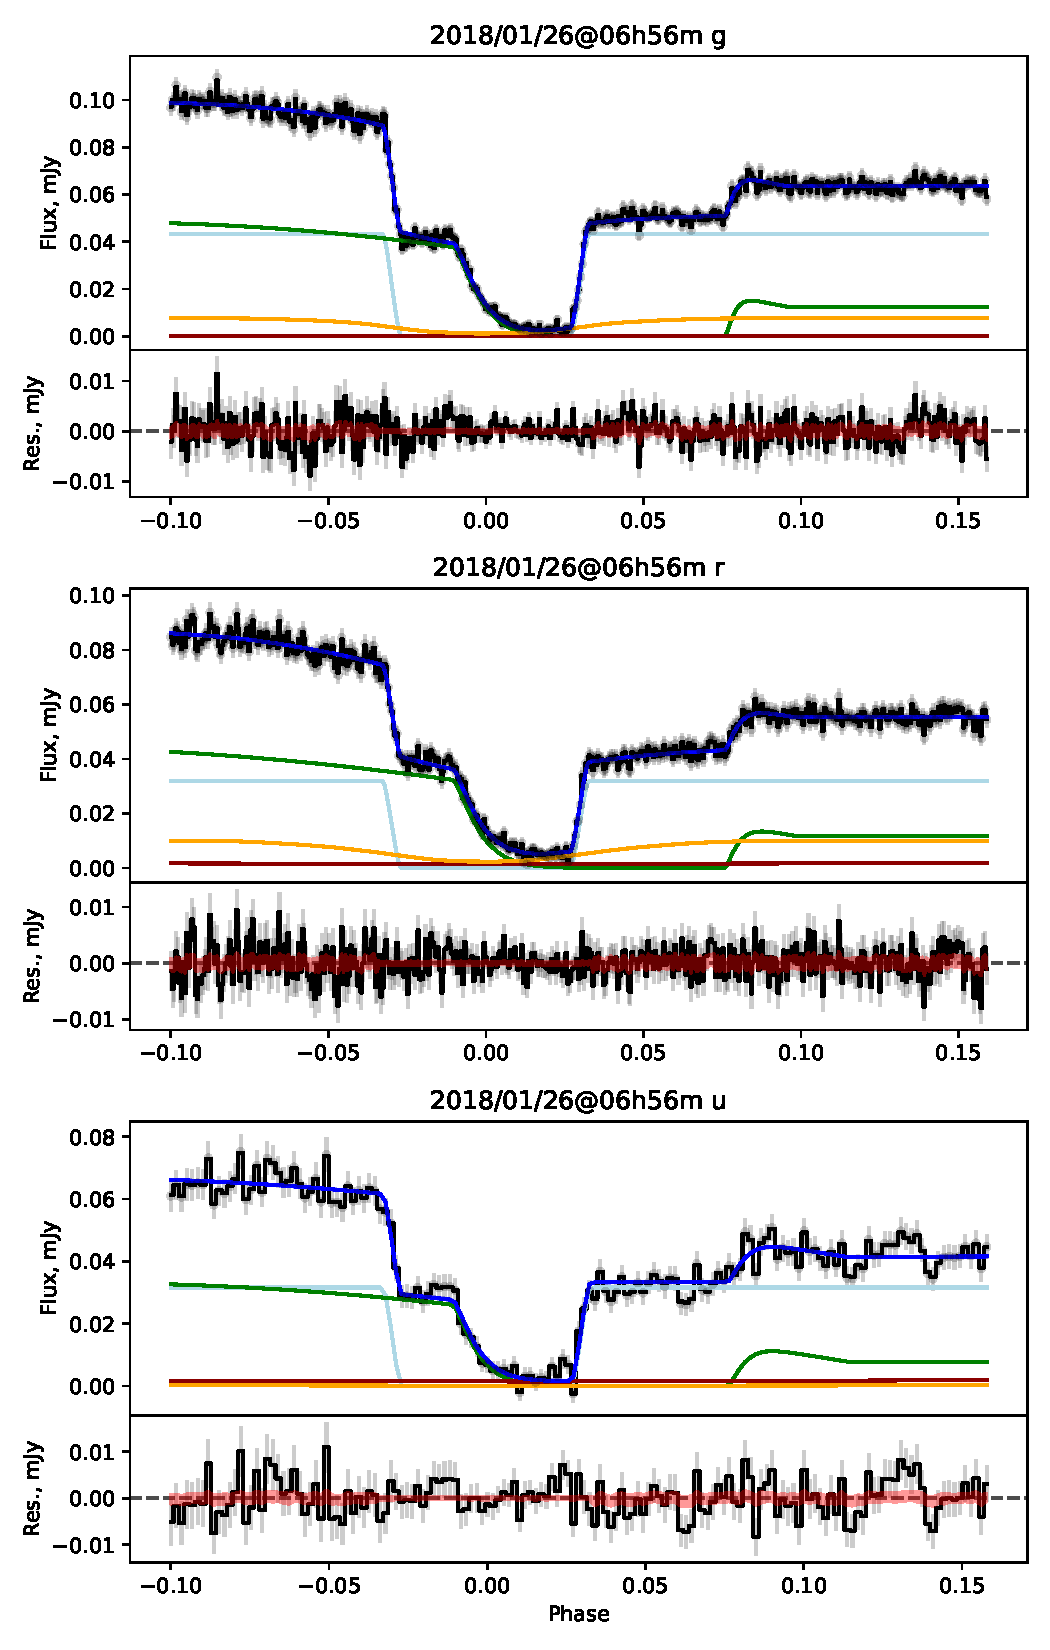
\includegraphics[width=\textwidth]{figures/results/ASASSN-17fo/ASASSN-17fo_3.pdf}
    \caption{ASASSN-17fo light curve models (cont.)}
    \label{fig:ASASSN-17fo all light curves cont 2}
\end{figure}
\begin{figure}
    \centering
    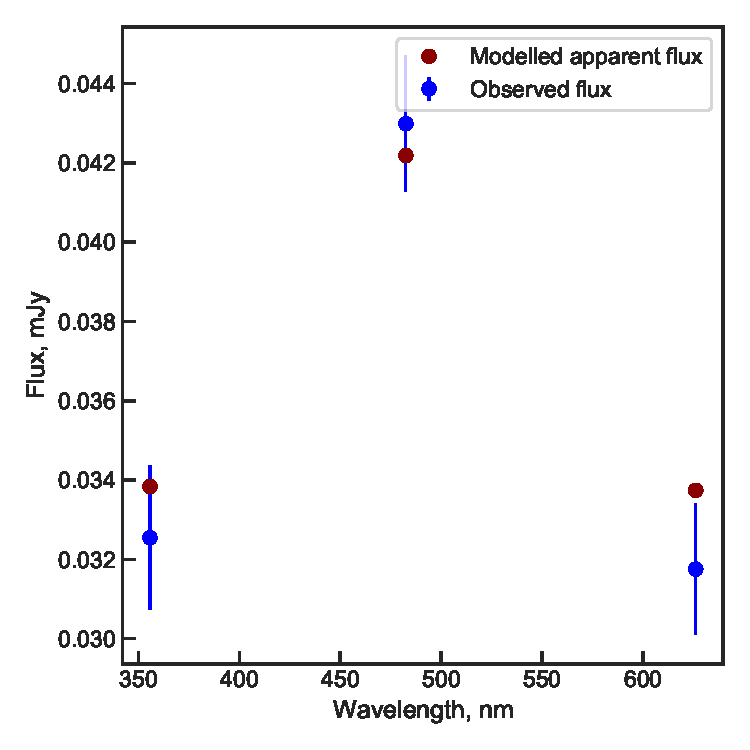
\includegraphics[width=\textwidth]{figures/results/ASASSN-17fo/fluxplot.pdf}
    \caption{ASASSN-17fo observed white dwarf fluxes, compared to the best-fit model atmosphere.}
    \label{fig:ASASSN-17fo flux plot}
\end{figure}
\clearpage




\newpage
\subsection{AY For}

AY For had the white dwarf and donor stars' masses estimated spectroscopically in \citet{mason2005} to be $M_{\rm wd} \sim 0.64 M_\odot$ and $M_{\rm donor} \sim 0.17 M_\odot$, with no error reported.
These values are not consistent with my findings of $M_{\rm wd} = 0.78\pm0.02 M_\odot$ and $M_{\rm donor} = 0.106\pm0.006 M_\odot$.
The previous measurement is highly dubious; it is based on inferring a donor mass and radius from the period using the model $M_{\rm donor} - P$ relation presented in \citet{howell2002}, which is then used to calculate a white dwarf mass from a spectroscopic $q$. This relies heavily on a poorly understood relationship, and extrapolates that further when giving a white dwarf mass.
AY For is also claimed by \citet{mason2005} to be a pre-period minimum system, which is corroborated by this more rigorous analysis.

The white dwarf fluxes of AY For were not well-described by the white dwarf cooling tracks, similarly to the systems in \S\ref{sect:three white dwarfs:method wd atmosphere fits}. There is high confidence that this is a real effect rather than a poor calibration, as the field about AY For was observed by the PANSTARRS survey, and the comparison star SDSS magnitudes are reported, which can be used to flux-calibrate the data independently of the standard star method typically used. Comparing these two calibrations finds comparison star fluxes that are within 2\% of each other. Rather, this system possibly suffers from a similar corrupting effect to that seen in the three CVs of Chapter~\ref{chpt:three peculiar white dwarfs}, though the disagreement here is not as severe as the extreme case of SSSJ0522$-$3505. Modelling error is similarly unlikely, as the light curve fits generally show distinct ingress and egress features that are replicated in the models. However, based on the in-depth analysis of Chapter~\ref{chpt:three peculiar white dwarfs}, the system parameters of AY For can still be considered robust.


% \begin{landscape}
%     \begin{table}
	\begin{center}
		\caption{Observations taken for AY For.}
		\label{table:observing:observation logs AYFor}
		\begin{tabular}{ccccccccc}
			\hline
			Instrument & Telescope & Date & Observation  & Observation  & Filter(s) & $T_{\rm ecl}$ & Cycle No. & Binning \\
			 &  &  &  start &  end &  &  &  & ID \\
			 &  &  & TDB & TDB &  & MJD &  &  \\
			\hline
			\hline
			UCAM & NTT & 2016/11/09 & 01:57 & 03:02 & $u_{\rm reg},g_{\rm reg},r_{\rm reg}$ & 57701.10964(1) & -0 & - \\
			UCAM & NTT & 2016/11/10 & 03:09 & 03:53 & $u_{\rm reg},g_{\rm reg},r_{\rm reg}$ & 57702.15423(1) & 14 & - \\
			UCAM & NTT & 2016/11/11 & 02:34 & 03:12 & $u_{\rm reg},g_{\rm reg},r_{\rm reg}$ & 57703.12424(1) & 27 & - \\
		   \hline
		\end{tabular}
	\end{center}
\end{table}
% \end{landscape}

\begin{figure}
    \centering
    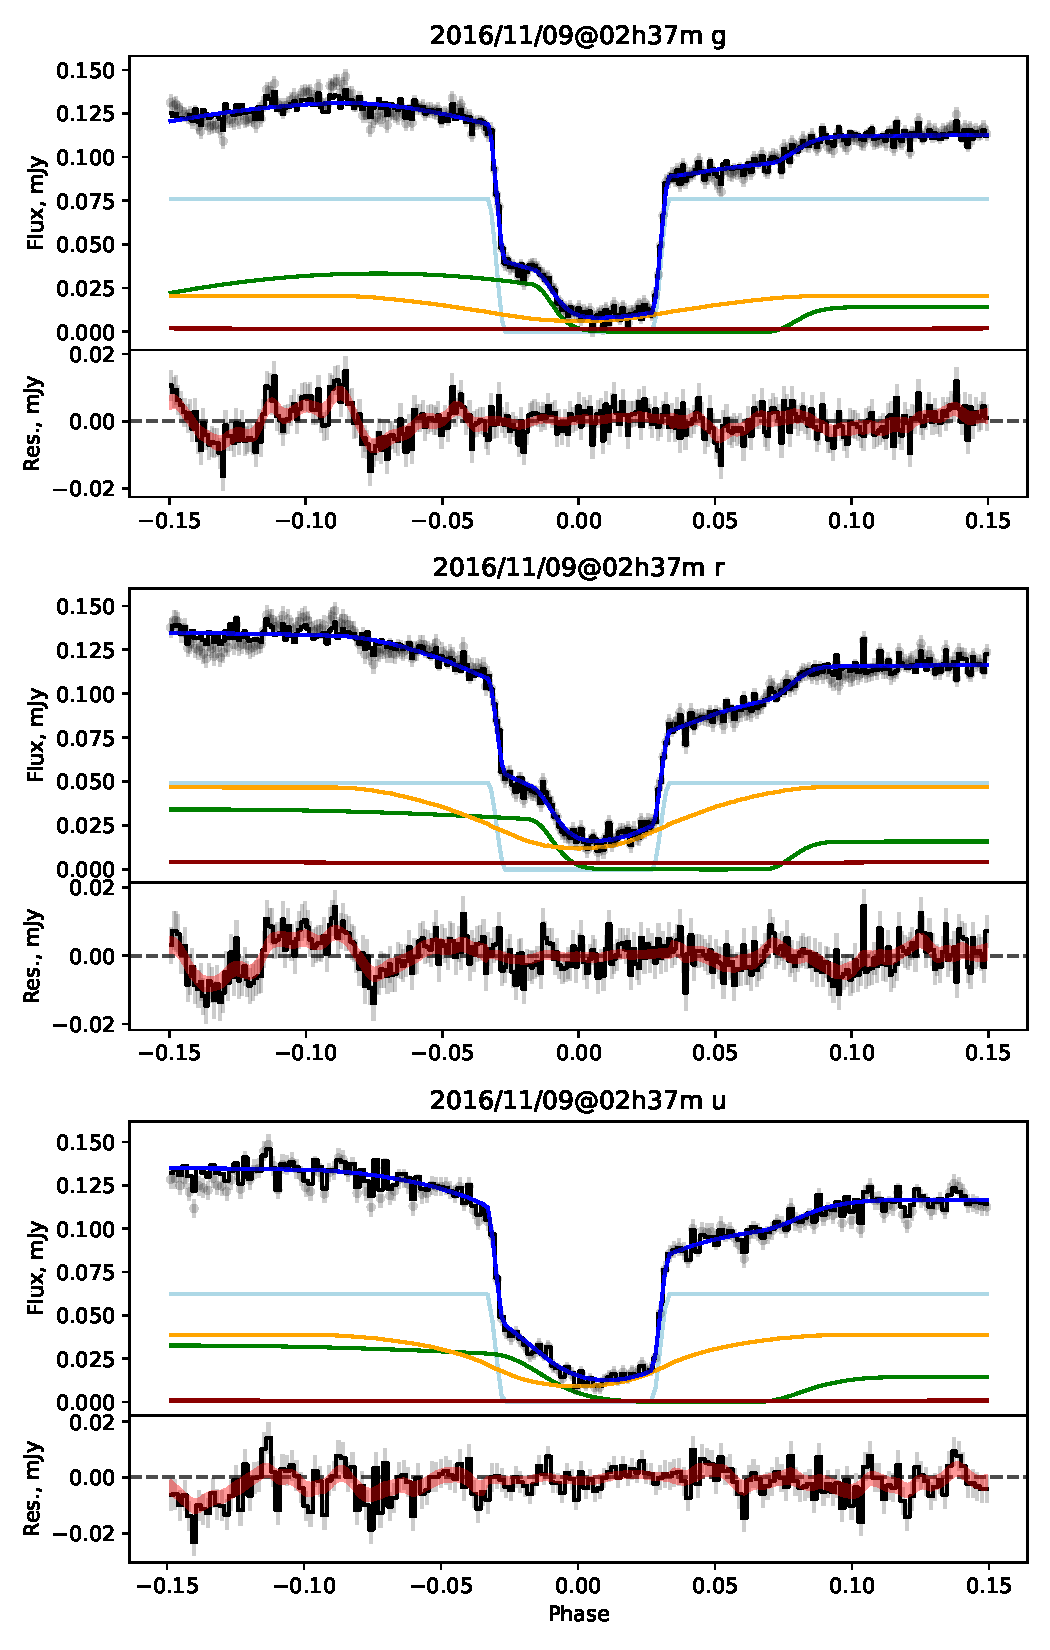
\includegraphics[width=\textwidth]{figures/results/AYFor/AYFor_1.pdf}
    \caption{AY For light curve models. Symbols are the same as Figure~\ref{fig:ASASSN-17jf all light curves}}
    \label{fig:AYFor all light curves}
\end{figure}
\begin{figure}
    \centering
    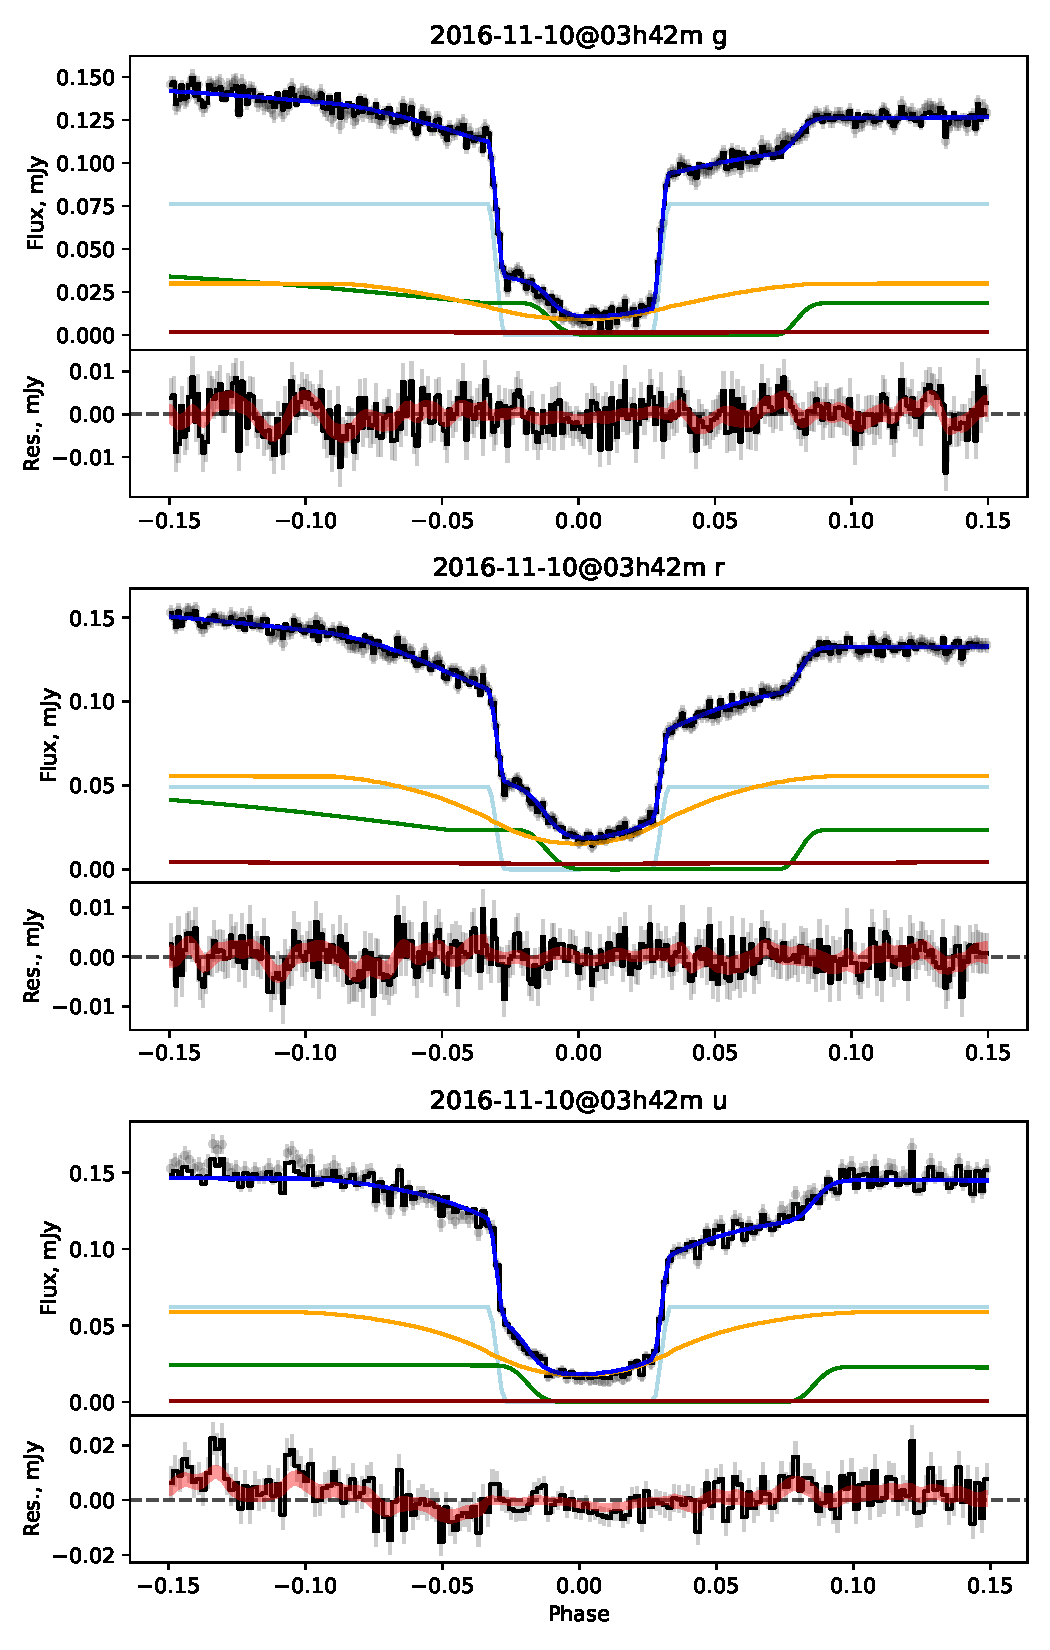
\includegraphics[width=\textwidth]{figures/results/AYFor/AYFor_2.pdf}
    \caption{AY For light curve models (cont.)}
    \label{fig:AYFor all light curves cont 1}
\end{figure}
\begin{figure}
    \centering
    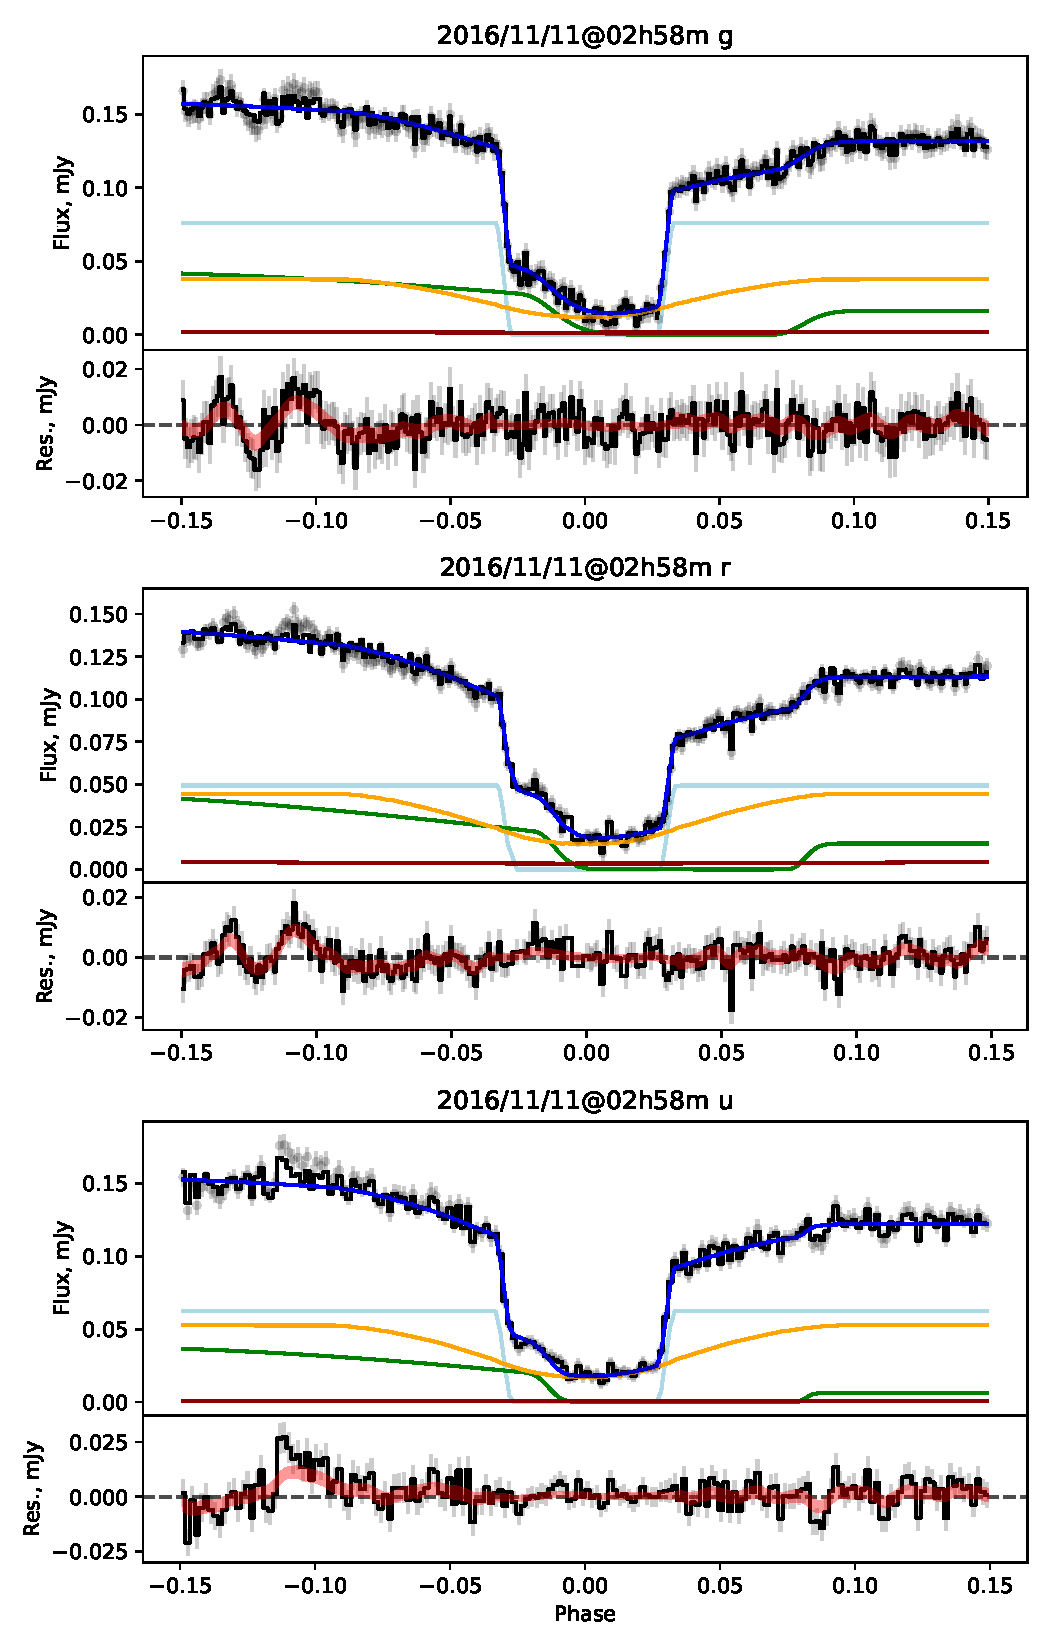
\includegraphics[width=\textwidth]{figures/results/AYFor/AYFor_3.pdf}
    \caption{AY For light curve models (cont.)}
    \label{fig:AYFor all light curves cont 2}
\end{figure}
\begin{figure}
    \centering
    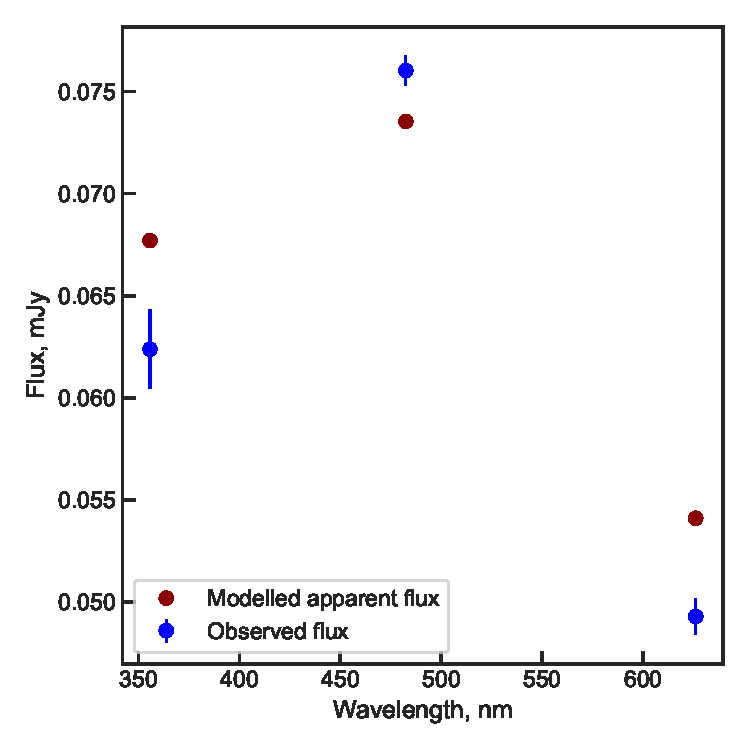
\includegraphics[width=\textwidth]{figures/results/AYFor/fluxplot.pdf}
    \caption{AY For observed white dwarf fluxes, compared to the best-fit model atmosphere.}
    \label{fig:AYFor flux plot}
\end{figure}
\clearpage



\newpage
\subsection{CSS090102}

Despite these observations spanning three years, from May 2011 to August 2014, the eclipses were concordant enough to be binned together.
The resulting data have somewhat weak bright spot egress features, but the optimised eclipse model reproduces the observation well, with very little residual scatter about the model.
The white dwarf fluxes are again well-described by cooling tracks, producing a relatively low but reasonable $M_\mathrm{wd} = 0.62\pm0.03 M_\odot$ and the best-fit parallax of $1.41\pm0.30$~mas again agrees well with the Gaia observation of $\pi = 1.51\pm0.32$~mas.

The best-fit system parameters place this CV at the donor mass at which the direction of period evolution begins to reverse. However, the observed period is significantly longer than the canonical period minimum, possibly indicating a significantly higher mass loss rate than is typical. Unfortunately, the donor mass is just below the threshold for the methodology of \S\ref{sect:modelling:evolutionary modelling} at $M_{\rm donor} = 0.060\pm0.003 M_\odot$, so this currently cannot be verified.


% \begin{landscape}
%     \begin{table}
	\begin{center}
		\caption{Observations taken for CSS090102. Mid-eclipse times and cycle numbers are calculated following the method detailed in \S\ref{sect:modelling:getting ephemeris}.}
		\label{table:observing:observation logs CSS090102}
		\begin{tabular}{cccccccc}
			\hline
			Instrument & Telescope & Date & Observation start & Observation end & Filter(s) & $T_{\rm ecl}$ & Cycle No. \\
				&  &  & UTC & UTC &  & BMJD &  \\
			\hline
			\hline
			UCAM & WHT & 2011/5/30 & 23:30 & 23:49 & $u_{\rm reg},g_{\rm reg},r_{\rm reg}$ & 55711.98538(2)                                                                                                            &                                       -3705 \\
			UCAM & WHT & 2011/6/2  & 00:23 & 01:38 & $u_{\rm reg},g_{\rm reg},r_{\rm reg}$ & 55714.04408(2)                                                                                                            &                                       -3672 \\
			UCAM & WHT & 2011/6/2  & 01:38 & 02:41 & $u_{\rm reg},g_{\rm reg},r_{\rm reg}$ & 55714.10647(2)                                                                                                            &                                       -3671 \\
			UCAM & WHT & 2012/1/17 & 02:28 & 03:18 & $u_{\rm reg},g_{\rm reg},r_{\rm reg}$ & 55943.12147(4)                                                                                                            &                                           0 \\
			UCAM & WHT & 2012/1/17 & 05:16 & 06:11 & $u_{\rm reg},g_{\rm reg},r_{\rm reg}$ & 55943.24624(2)                                                                                                            &                                           2 \\
			UCAM & WHT & 2014/8/4  & 21:01 & 21:58 & $u_{\rm reg},g_{\rm reg},r_{\rm reg}$ & 56873.90433(4)                                                                                                            &                                       14920 \\
		   \hline
		\end{tabular}
	\end{center}
\end{table}
% \end{landscape}

\begin{figure}
    \centering
    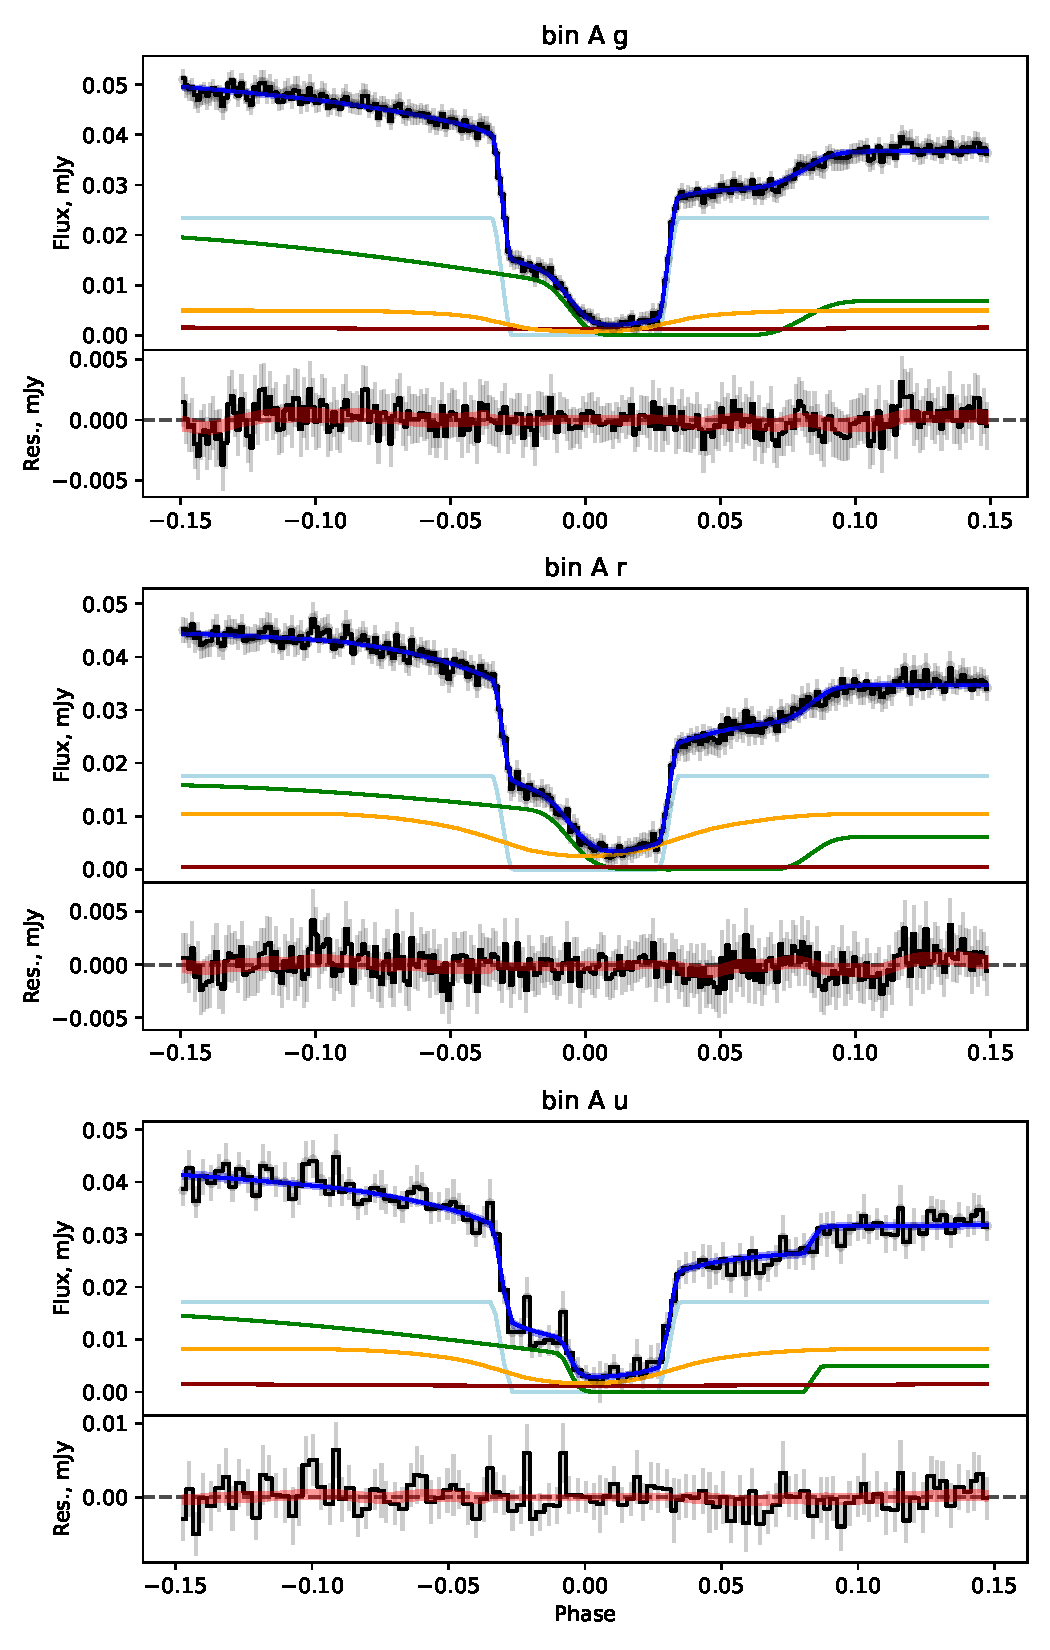
\includegraphics[width=\textwidth]{figures/results/CSS090102/CSS090102_1.pdf}
    \caption{CSS090102 light curve models. Symbols are the same as Figure~\ref{fig:ASASSN-17jf all light curves}. Data are the results of binning all available eclipses.}
    \label{fig:CSS090102 all light curves}
\end{figure}
\begin{figure}
    \centering
    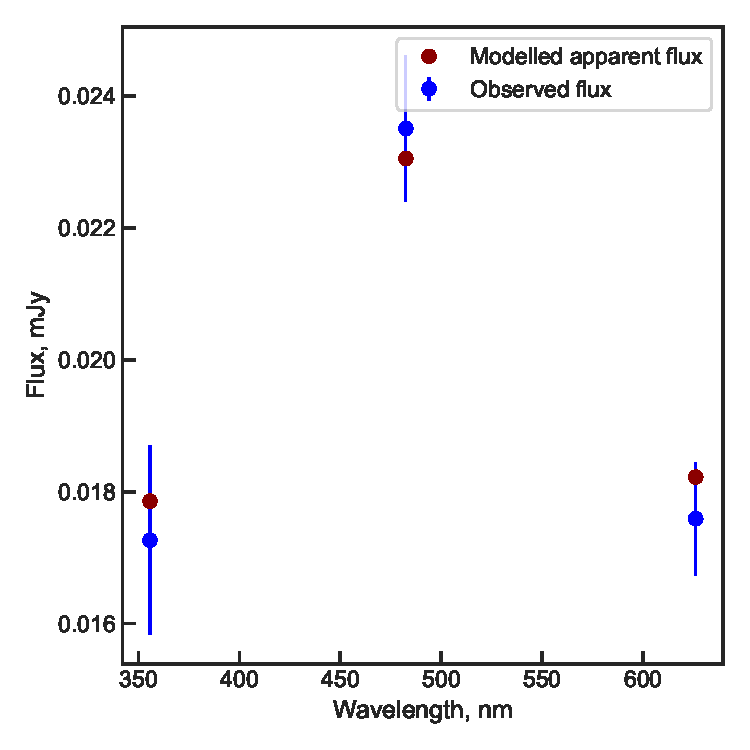
\includegraphics[width=\textwidth]{figures/results/CSS090102/fluxplot.pdf}
    \caption{CSS090102 observed white dwarf fluxes, compared to the best-fit model atmosphere.}
    \label{fig:CSS090102 flux plot}
\end{figure}
\clearpage




\newpage
\subsection{CSS090419}

The white dwarf of CSS090419 significantly brightens in the $i'$ band, compared to the $r'$ band. This is unlikely to be calibration error in the $i'$ band, as calibration has otherwise proven to be robust. In addition, this brightening is not seen in the ASASSN-15pb $i'$ band observations, suggesting it is not a systematic issue.

The resulting fit appears to be acceptable, with little residual flux. These fits are given in Figures~\ref{fig:CSS090419 all light curves}~and~\ref{fig:CSS090419 all light curves cont 1}, and show that the eclipse model does a good job of describing the data.
However, the white dwarf and bright spot ingresses are somewhat blended in the $r'$ and $i'$, and whilst the egresses are distinct enough to resolve a white dwarf flux, the key parameters of $R_{\rm wd}$ and $\Delta \phi$ are more difficult to constrain.
In addition, inspecting the light curves shows that there is some level of degeneracy between the disc flux and white dwarf flux, particularly in the $r'$ band, exacerbating the difficulty in modelling.
These blended features are reflected in large uncertainty in white dwarf flux. Indeed, the standard deviations on all four white dwarf fluxes are large enough that they are consistent with their mean -- a perfectly flat spectrum.

This is not typical white dwarf behaviour, and cannot be reproduced by the white dwarf model atmospheres used here given the constraints. Whilst an extremely hot white dwarf is able to produce a flat spectrum in the optical range, the luminosity of such an object is forbidden by the Gaia distance measurement.
This preference for a flat spectrum is reflected in the high, and highly uncertain, best fit $T_{\rm eff} = 18200 \pm 9000$K, though the posterior $\pi$ distribution is consistent with the Gaia measurement of $1.41\pm0.78$ mas, with slightly reduced uncertainty. Also note that this system appears to have the lowest white dwarf mass of the sample, of only $0.59\pm0.08 M_\odot$.
Despite these issues with the white dwarf fitting, as demonstrated in Chapter~\ref{chpt:three peculiar white dwarfs} the uncertain white dwarf model has little impact on the system parameters, and the resulting characterisation can still be considered valid.


% \begin{landscape}
%     \begin{table}
	\begin{center}
		\caption{Observations taken for CSS090419.}
		\label{table:observing:observation logs CSS090419}
		\begin{tabular}{ccccccccc}
			\hline
			Instrument & Telescope & Date & Observation  & Observation  & Filter(s) & $T_{\rm ecl}$ & Cycle No. & Binning \\
			 &  &  &  start &  end &  &  &  & ID \\
			 &  &  & TDB & TDB &  & MJD &  &  \\
			\hline
			\hline
			UCAM & WHT & 2013/25/7 & 21:41 & 22:38 & $u_{\rm reg},g_{\rm reg},i_{\rm reg}$ & 56498.92854(2) &    0  & A \\
			UCAM & WHT & 2013/26/7 & 21:05 & 22:00 & $u_{\rm reg},g_{\rm reg},r_{\rm reg}$ & 56499.90935(3) &   13  & A \\
			UCAM & WHT & 2013/28/7 & 22:12 & 23:02 & $u_{\rm reg},g_{\rm reg},i_{\rm reg}$ & 56501.94632(7) &   40  & A \\
			UCAM & WHT & 2013/4/8  & 21:00 & 21:30 & $u_{\rm reg},g_{\rm reg},r_{\rm reg}$ & 56508.88704(3) &  132  & A \\
			UCAM & WHT & 2013/4/8  & 22:55 & 23:21 & $u_{\rm reg},g_{\rm reg},r_{\rm reg}$ & 56508.96244(3) &  133  & A \\
			UCAM & WHT & 2014/3/8  & 20:59 & 21:50 & $u_{\rm reg},g_{\rm reg},r_{\rm reg}$ & 56872.89819(3) & 4957  & A \\
			UCAM & NTT & 2021/9/7  & 03:26 & 04:00 & $u_{\rm sup},g_{\rm sup},i_{\rm sup}$ & 59404.15373(6) & 38509 & A \\
			UCAM & NTT & 2021/10/7 & 04:30 & 05:10 & $u_{\rm sup},g_{\rm sup},i_{\rm sup}$ & 59405.21005(7) & 38523 & A \\
		   \hline
		\end{tabular}
	\end{center}
\end{table}
% \end{landscape}

\begin{figure}
    \centering
    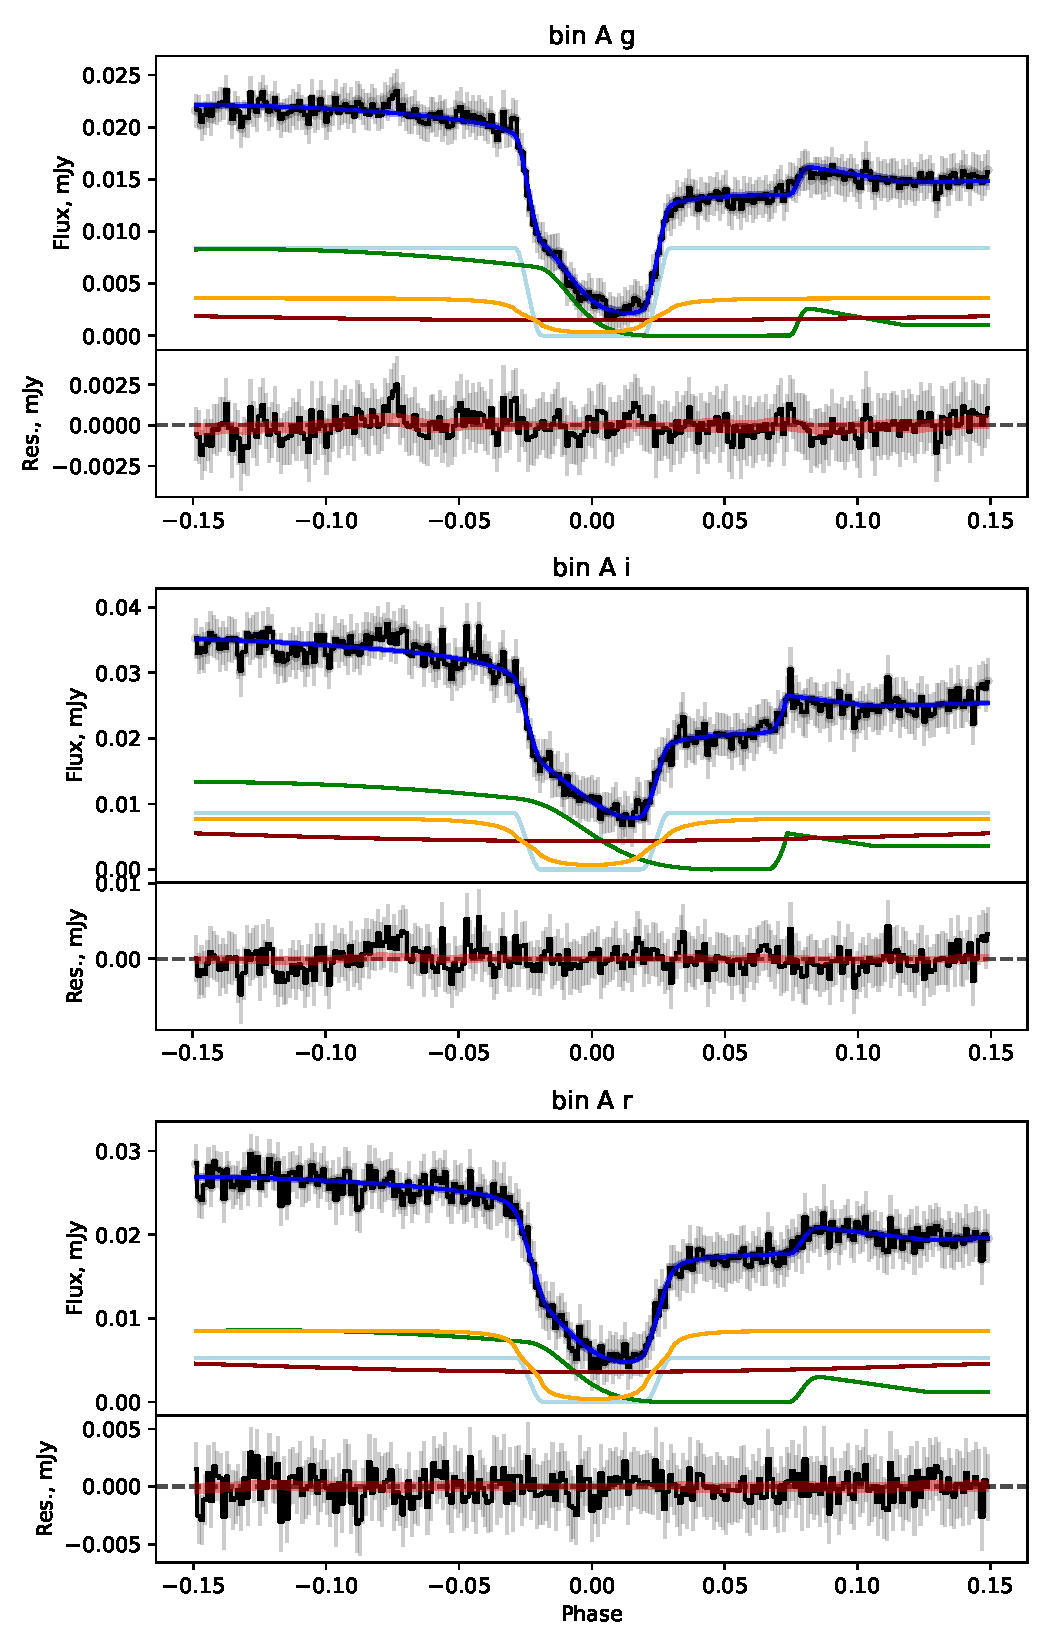
\includegraphics[width=\textwidth]{figures/results/CSS090419/CSS090419_1.pdf}
    \caption{CSS090419 light curve models. Symbols are the same as Figure~\ref{fig:ASASSN-17jf all light curves}. Data are the results of binning all available eclipses.}
    \label{fig:CSS090419 all light curves}
\end{figure}
\begin{figure}
    \centering
    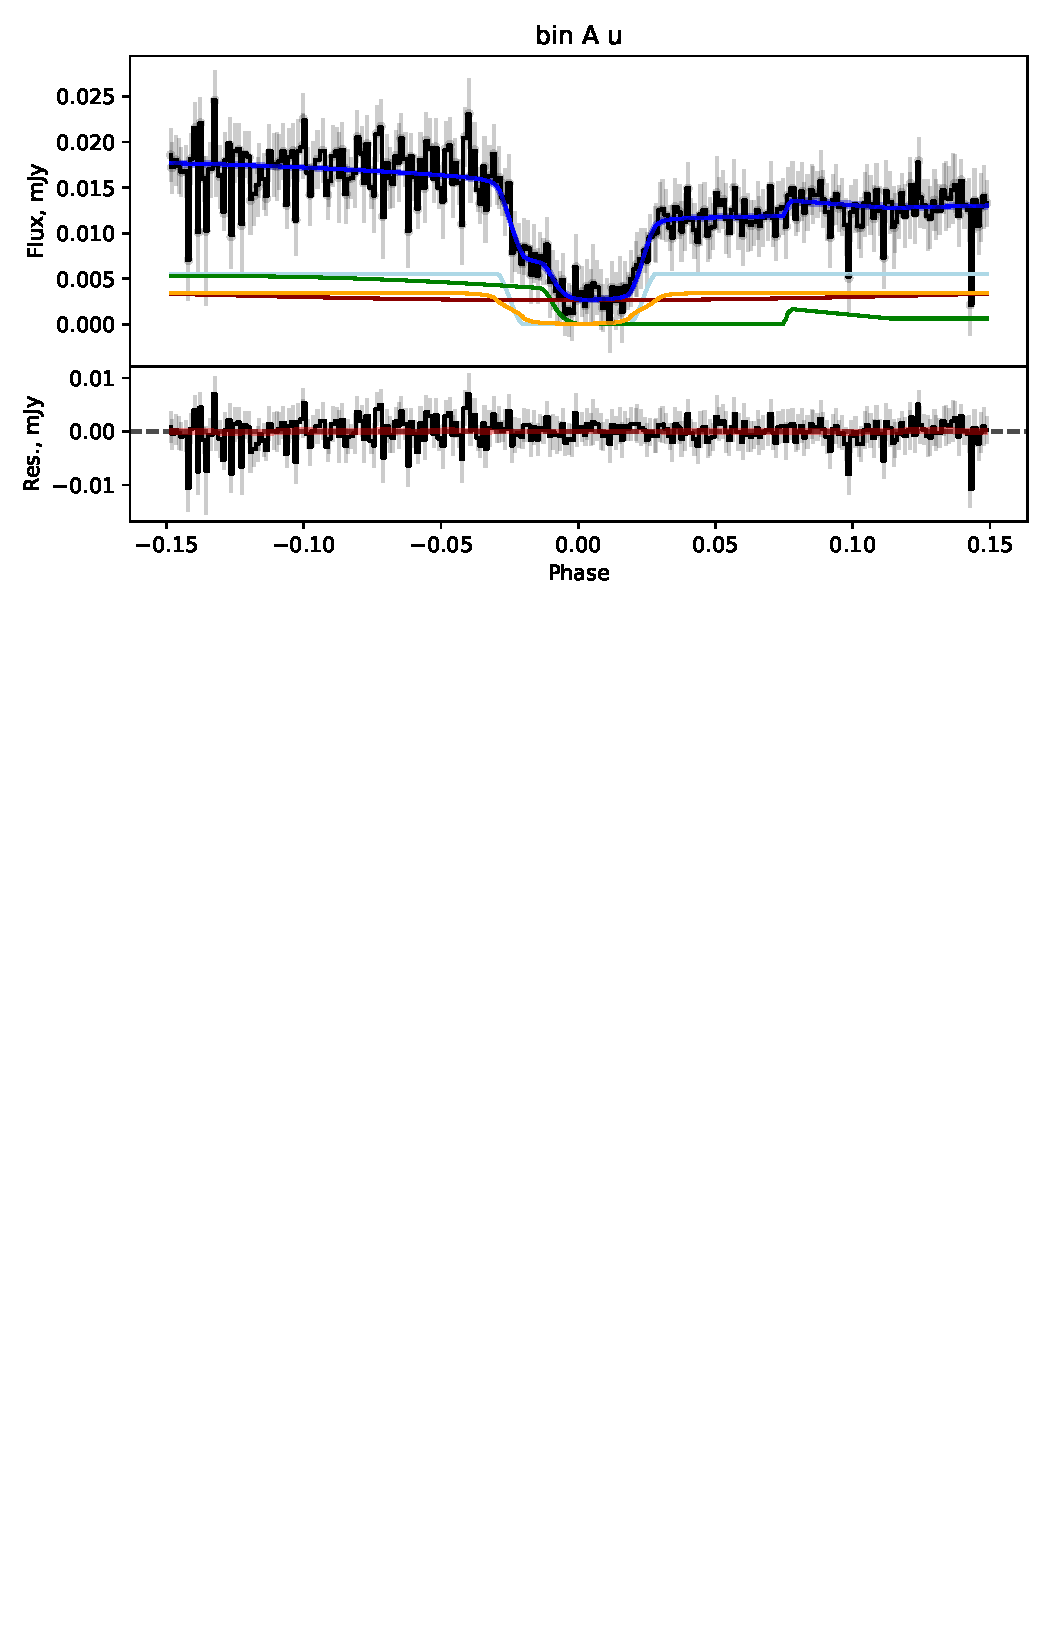
\includegraphics[width=\textwidth, trim={0cm 17cm 0cm 0cm}, clip]{figures/results/CSS090419/CSS090419_2.pdf}
    \caption{CSS090419 light curve models (cont.). Data are the results of binning all available eclipses.}
    \label{fig:CSS090419 all light curves cont 1}
\end{figure}
\begin{figure}
    \centering
    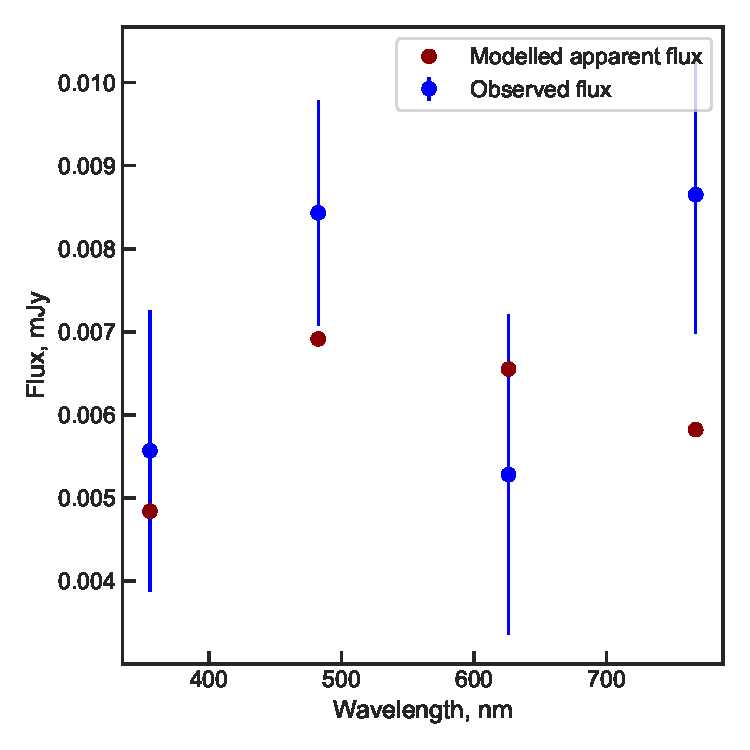
\includegraphics[width=\textwidth]{figures/results/CSS090419/fluxplot.pdf}
    \caption{CSS090419 observed white dwarf fluxes, compared to the best-fit model atmosphere.}
    \label{fig:CSS090419 flux plot}
\end{figure}
\clearpage



\newpage
\subsection{CSS090622}

These observations fell into two binning categories, due to a significant dimming of the disc by a factor of $\sim 3$ between 2014/8/5 and 2014/8/8. Note that all eclipses (except the bin A $u'$ eclipse) show a slight dip in flux before white dwarf ingress, possibly due to some absorbing feature in the disc.
Whilst both data sets are suitable for modelling, with eclipse features that are distinct enough to characterise, the post-disc-dimming data are significantly improved, with clear, sharp ingresses and egresses. Without the improved feature resolution, this system would be significantly more challenging to model due to the severely blended $u'$ band eclipse in the bin A eclipses.

The resulting white dwarf flux fit is acceptable, converging on $\pi = 2.02\pm0.27$~mas to agree with the Gaia $\pi=2.08\pm0.27$~mas, and finding a white dwarf mass of $0.67\pm0.06 M_\odot$. The period and donor mass are consistent with the `optimal' \citet{knigge11} donor track.

% \begin{landscape}
%     \begin{table}
	\begin{center}
		\begin{tabular}{cccccccc}
			\hline
			Instrument & Telescope & Date & Observation start & Observation end & Filter(s) & $T_{\rm ecl}$ & Cycle No. \\
			 &  &  & UTC & UTC &  & BMJD &  \\
			\hline
			\hline
			UCAM & WHT & 2014/8/5  & 02:31 & 03:20 & $u_{\rm reg},g_{\rm reg},r_{\rm reg}$ & 56874.13102(5)                                                                                                            &                                          -1 \\
			UCAM & WHT & 2014/8/5  & 04:34 & 04:58 & $u_{\rm reg},g_{\rm reg},r_{\rm reg}$ & 56874.20195(5)                                                                                                            &                                           0 \\
			UCAM & WHT & 2014/8/5  & 23:07 & 23:43 & $u_{\rm reg},g_{\rm reg},r_{\rm reg}$ & 56874.98217(5)                                                                                                            &                                          11 \\
			UCAM & WHT & 2014/8/8  & 22:31 & 23:10 & $u_{\rm reg},g_{\rm reg},i_{\rm reg}$ & 56877.96120(5)                                                                                                            &                                          53 \\
			UCAM & WHT & 2014/8/9  & 03:43 & 04:22 & $u_{\rm reg},g_{\rm reg},i_{\rm reg}$ & 56878.17399(5)                                                                                                            &                                          56 \\
			UCAM & WHT & 2014/8/11 & 04:50 & 05:37 & $u_{\rm reg},g_{\rm reg},i_{\rm reg}$ & 56880.23094(5)                                                                                                            &                                          85 \\
		   \hline
		\end{tabular}
	\end{center}
	\caption{Observations taken for CSS090622.}
	\label{table:observing:observation logs CSS090622}
\end{table}
% \end{landscape}

\begin{figure}
    \centering
    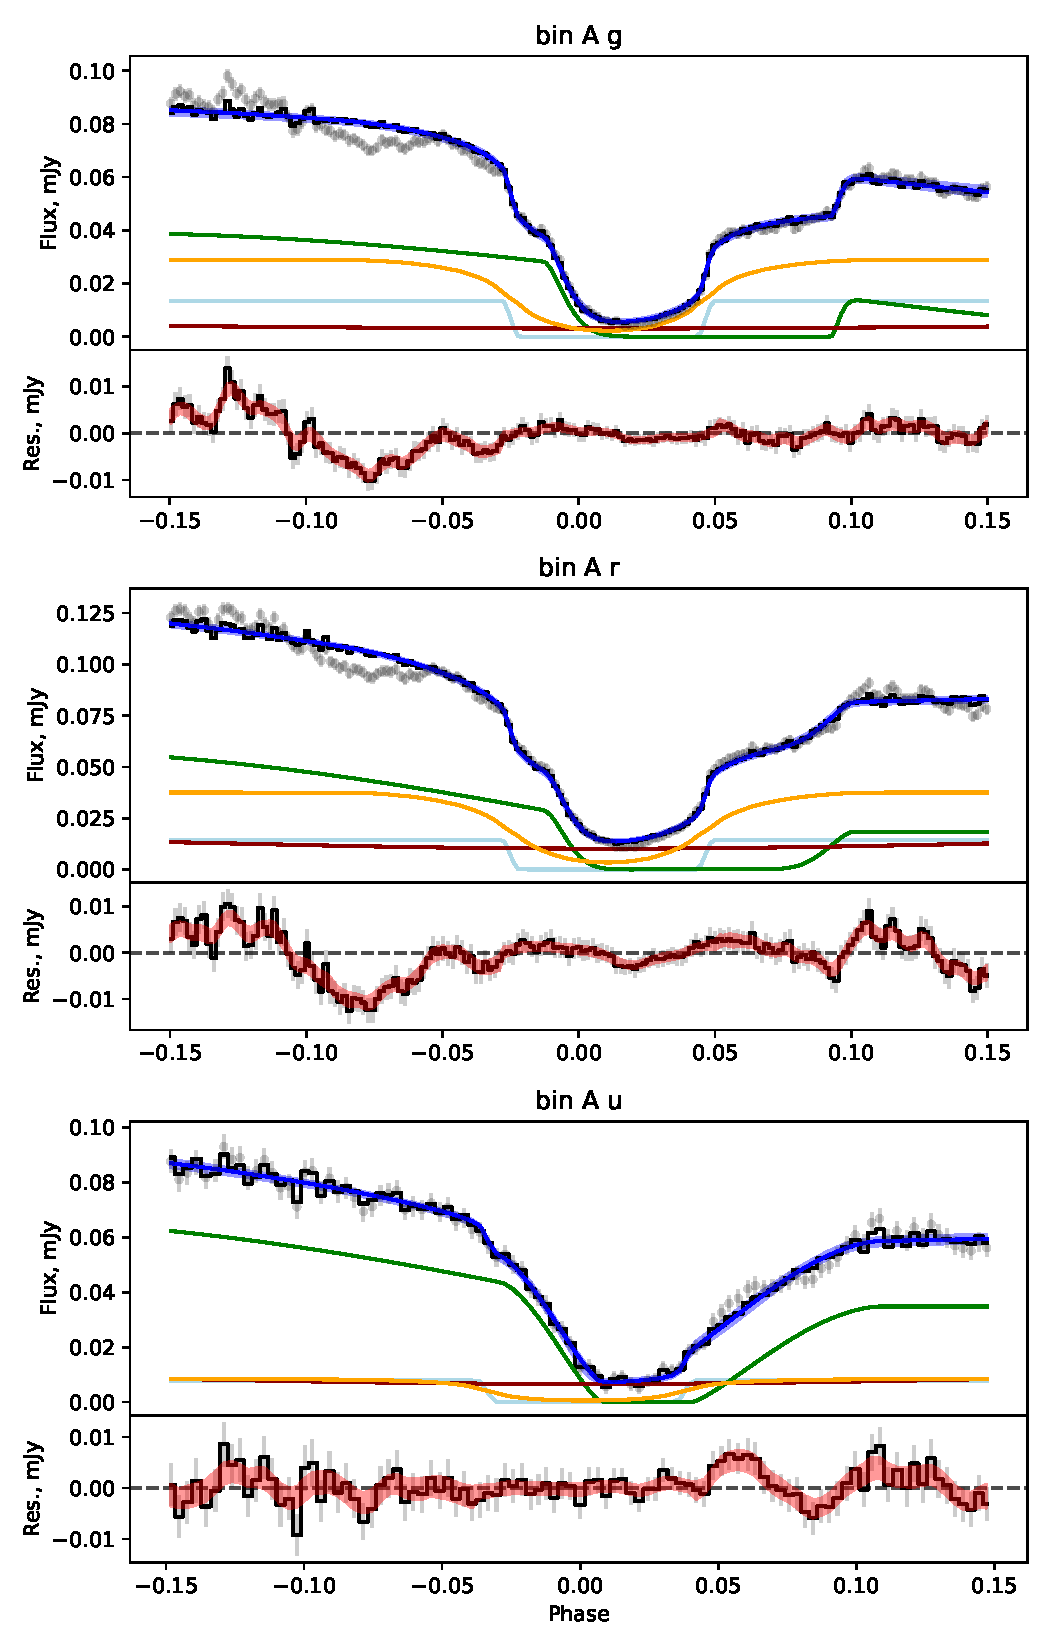
\includegraphics[width=\textwidth]{figures/results/CSS090622/CSS090622_1.pdf}
    \caption{CSS090622 light curve models. Symbols are the same as Figure~\ref{fig:ASASSN-17jf all light curves}. Data are the result of binning together the three eclipses of 2014/8/5.}
    \label{fig:CSS090622 all light curves}
\end{figure}
\begin{figure}
    \centering
    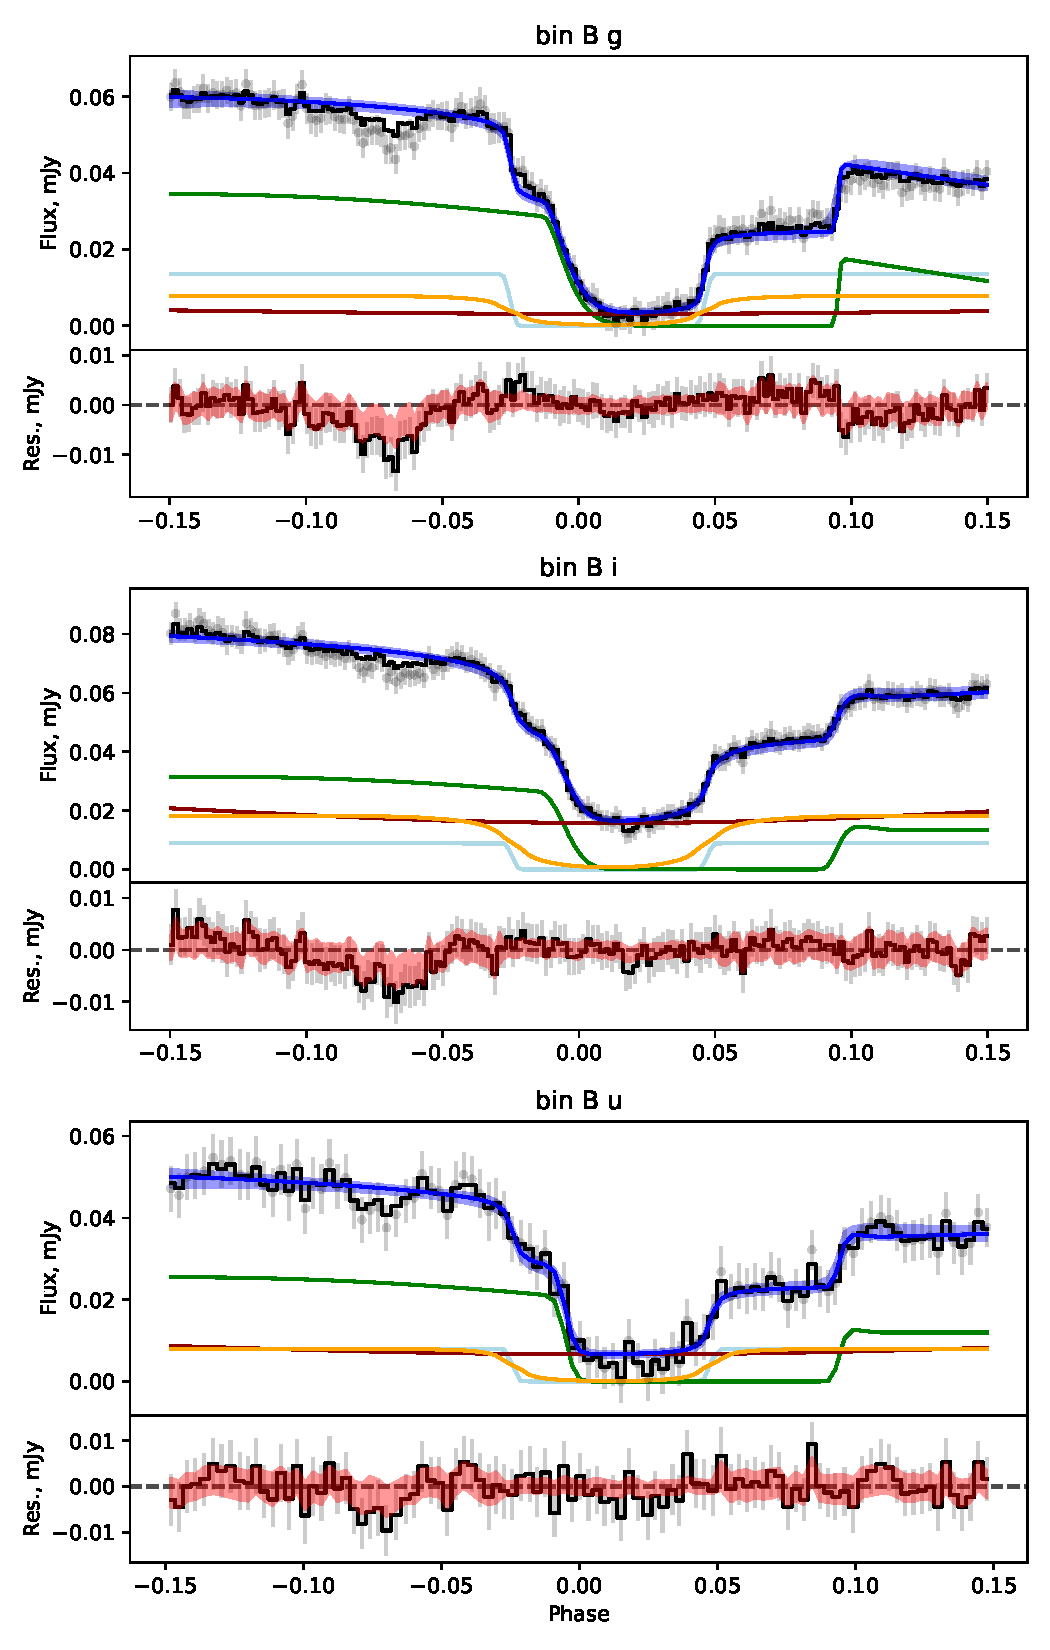
\includegraphics[width=\textwidth]{figures/results/CSS090622/CSS090622_2.pdf}
    \caption{CSS090622 light curve models (cont.). Data are the result of binning together the eclipses of 2014/8/8, 2014/8/9, 2014/8/11.}
    \label{fig:CSS090622 all light curves cont 1}
\end{figure}
\begin{figure}
    \centering
    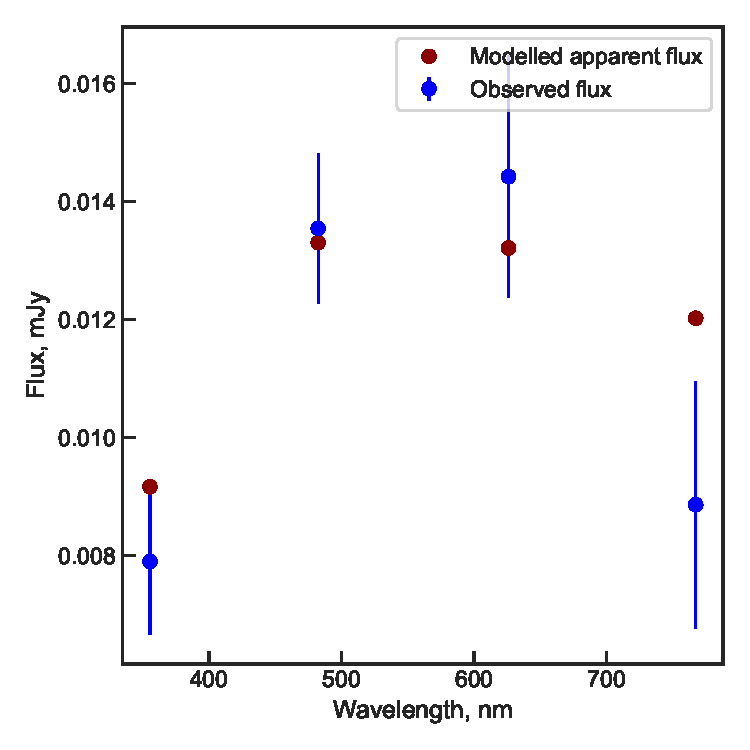
\includegraphics[width=\textwidth]{figures/results/CSS090622/fluxplot.pdf}
    \caption{CSS090622 observed white dwarf fluxes, compared to the best-fit model atmosphere.}
    \label{fig:CSS090622 flux plot}
\end{figure}
\clearpage



\newpage
\subsection{MASOT0014}

As this system has strong disc features and significant flickering, modelling was challenging. Flickering during white dwarf ingress and egress resulted in uncertain white dwarf flux measurements, and the weak bright spot egress was similarly masked, though the severity of this was reduced somewhat by the hierarchical model. In addition, this system is host to a significant disc, which can obscure the fainter bright spot features.
Despite this, the white dwarf fluxes are well-described by the cooling tracks, and Figure~\ref{fig:12 new cvs:donor model with eclipsers plotted} shows this system as consistent with the `standard' donor evolution track.
Further supporting the model fitting is the Gaia $\pi = 2.31 \pm 0.13$~mas, closely agreeing with the white dwarf atmosphere fitting value of $2.42\pm0.11$~mas.

% \begin{landscape}
%     \begin{table}
	\begin{center}
		\caption{Observations taken for MASTER OT J001400.25-561735.0.}
		\label{table:observing:observation logs MASTER OT J0014}
		\begin{tabular}{ccccccccc}
			\hline
			Instrument & Telescope & Date & Observation  & Observation  & Filter(s) & $T_{\rm ecl}$ & Cycle No. & Binning \\
			 &  &  &  start &  end &  &  &  & ID \\
			 &  &  & TDB & TDB &  & MJD &  &  \\
			\hline
			\hline
			% UCAM & WHT & 2014/8/5  & 02:31 & 03:20 & $u_{\rm reg},g_{\rm reg},r_{\rm reg}$ & 56874.13102(5) &  & A \\

            UCAM & NTT & 2016/8/25 & 05:28 & 07:36 & $u_{\rm reg},g_{\rm reg},r_{\rm reg}$ & 57625.29674(4)     & -11   & A \\
            UCAM & NTT & 2016/8/26 & 01:26 & 02:22 & $u_{\rm reg},g_{\rm reg},r_{\rm reg}$ & 57626.08356(7)     &   0   & A \\
            UCAM & NTT & 2016/11/8 & 02:39 & 03:04 & $u_{\rm reg},g_{\rm reg},r_{\rm reg}$ & 57700.116579(7)    & 1035  & - \\
            UCAM & NTT & 2017/6/12 & 10:07 & 10:30 & $u_{\rm reg},g_{\rm reg},r_{\rm reg}$ & 57916.42174(1)     & 4059  & - \\
		   \hline
		\end{tabular}
	\end{center}
\end{table}
% \end{landscape}

\begin{figure}
    \centering
    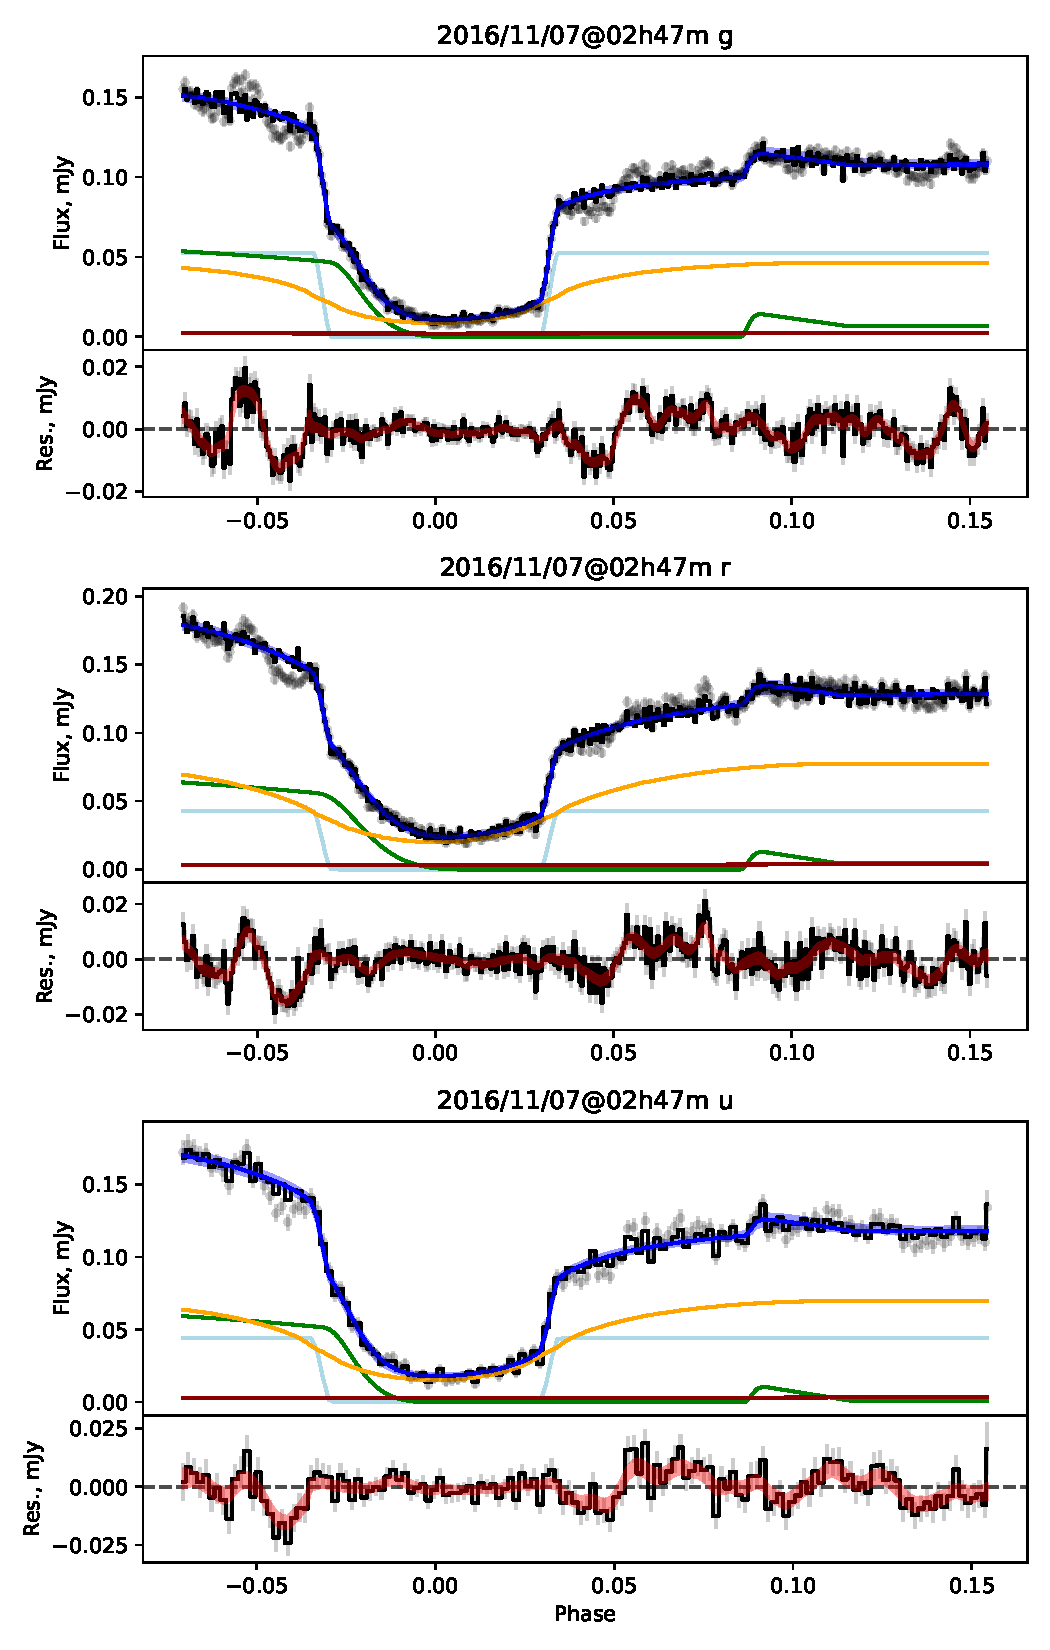
\includegraphics[width=\textwidth]{figures/results/MASOT0014/MASOT0014_1.pdf}
    \caption{MAS0014 light curve models. Symbols are the same as Figure~\ref{fig:ASASSN-17jf all light curves}.}
    \label{fig:MAS0014 all light curves}
\end{figure}
\begin{figure}
    \centering
    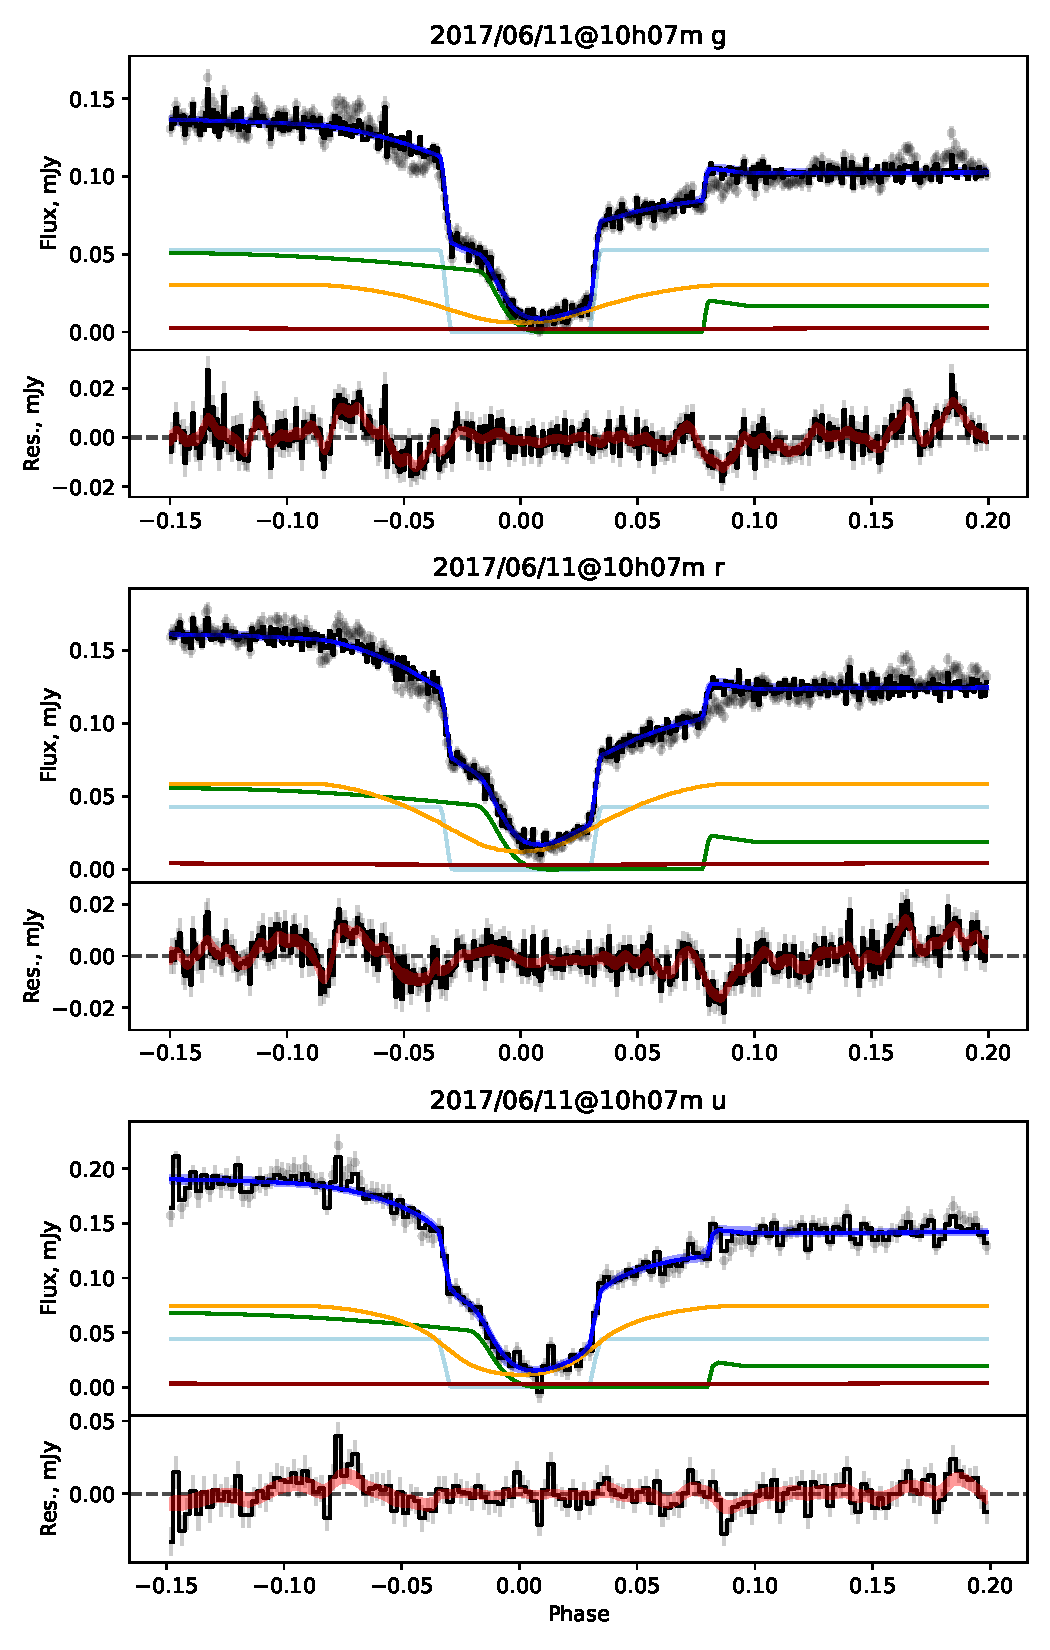
\includegraphics[width=\textwidth]{figures/results/MASOT0014/MASOT0014_2.pdf}
    \caption{MAS0014 light curve models (cont.)}
    \label{fig:MAS0014 all light curves cont 1}
\end{figure}
\begin{figure}
    \centering
    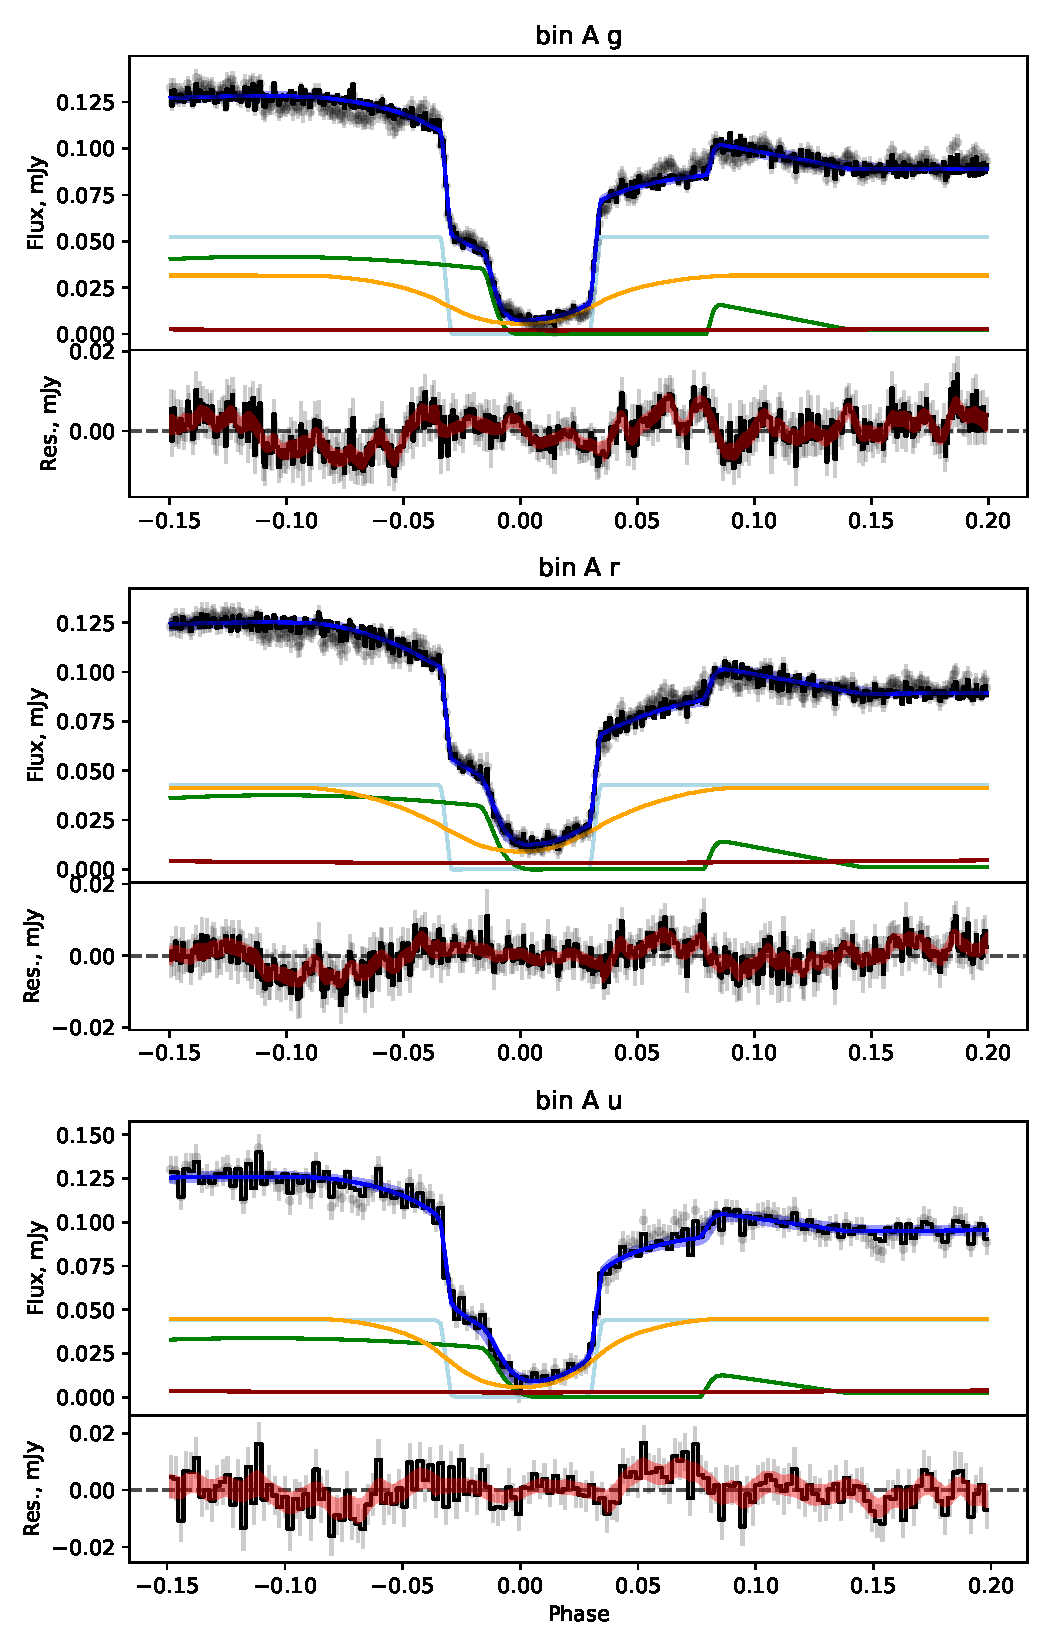
\includegraphics[width=\textwidth]{figures/results/MASOT0014/MASOT0014_3.pdf}
    \caption{MAS0014 light curve models (cont.). Data are the result of binning together the eclipses of 2016/8/25 and 2016/8/26.}
    \label{fig:MAS0014 all light curves cont 2}
\end{figure}
\begin{figure}
    \centering
    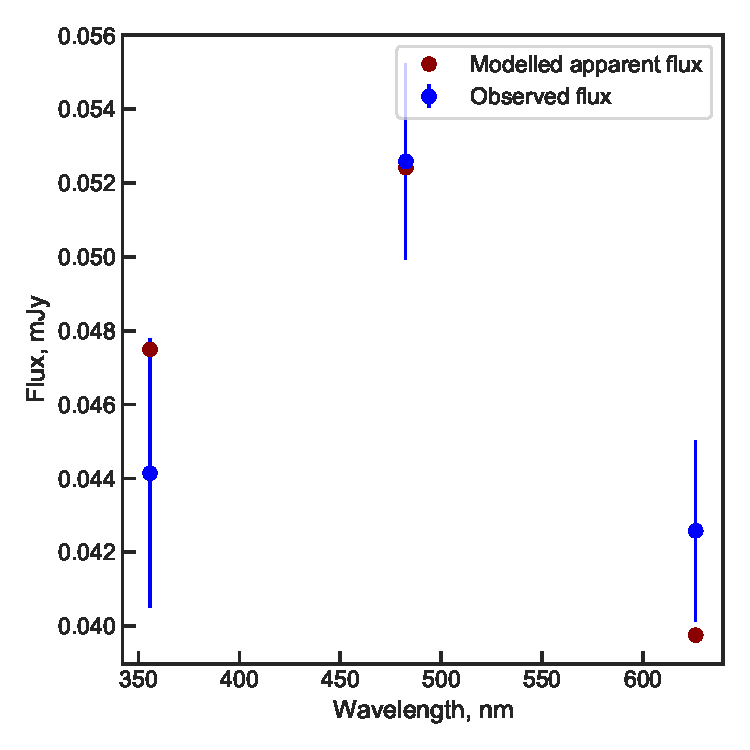
\includegraphics[width=\textwidth]{figures/results/MASOT0014/fluxplot.pdf}
    \caption{MAS0014 observed white dwarf fluxes, compared to the best-fit model atmosphere.}
    \label{fig:MAS0014 flux plot}
\end{figure}
\clearpage



\newpage
\subsection{OGLE82}

This system has only two observations, and 5 of the 6 resulting eclipses have distinct key eclipse features that make modelling significantly easier. The exception to this is the 2016/8/23 $u'$ band eclipse, which has a weak bright spot and so an obfuscated bright spot egress.
Most eclipses have significant flickering visible, which reduces as expected during the white dwarf eclipse, and appears to be generally less severe in the eclipse of 2016/8/23.
System parameters are well-constrained and sensible, with white dwarf fluxes that are reproduced by model cooling tracks and a donor mass that places this CV approximately $1\sigma$ above the `standard' donor track.


% \begin{landscape}
%     \begin{table}
	\begin{center}
		\caption{Observations taken for OGLE82.}
		\label{table:observing:observation logs OGLE82}
		\begin{tabular}{ccccccccc}
			\hline
			Instrument & Telescope & Date & Observation  & Observation  & Filter(s) & $T_{\rm ecl}$ & Cycle No. & Binning \\
			 &  &  &  start &  end &  &  &  & ID \\
			 &  &  & TDB & TDB &  & MJD &  &  \\
			\hline
			\hline
			UCAM & NTT & 2016/8/21 & 23:47 & 00:50 & $u_{\rm sup},g_{\rm sup},r_{\rm sup}$ & 57622.02757(1) & -14 & - \\
			UCAM & NTT & 2016/8/23 & 00:26 & 00:59 & $u_{\rm sup},g_{\rm sup},r_{\rm sup}$ & 57623.03460(1) &   0 & - \\
		   \hline
		\end{tabular}
	\end{center}
\end{table}
% \end{landscape}

\begin{figure}
    \centering
    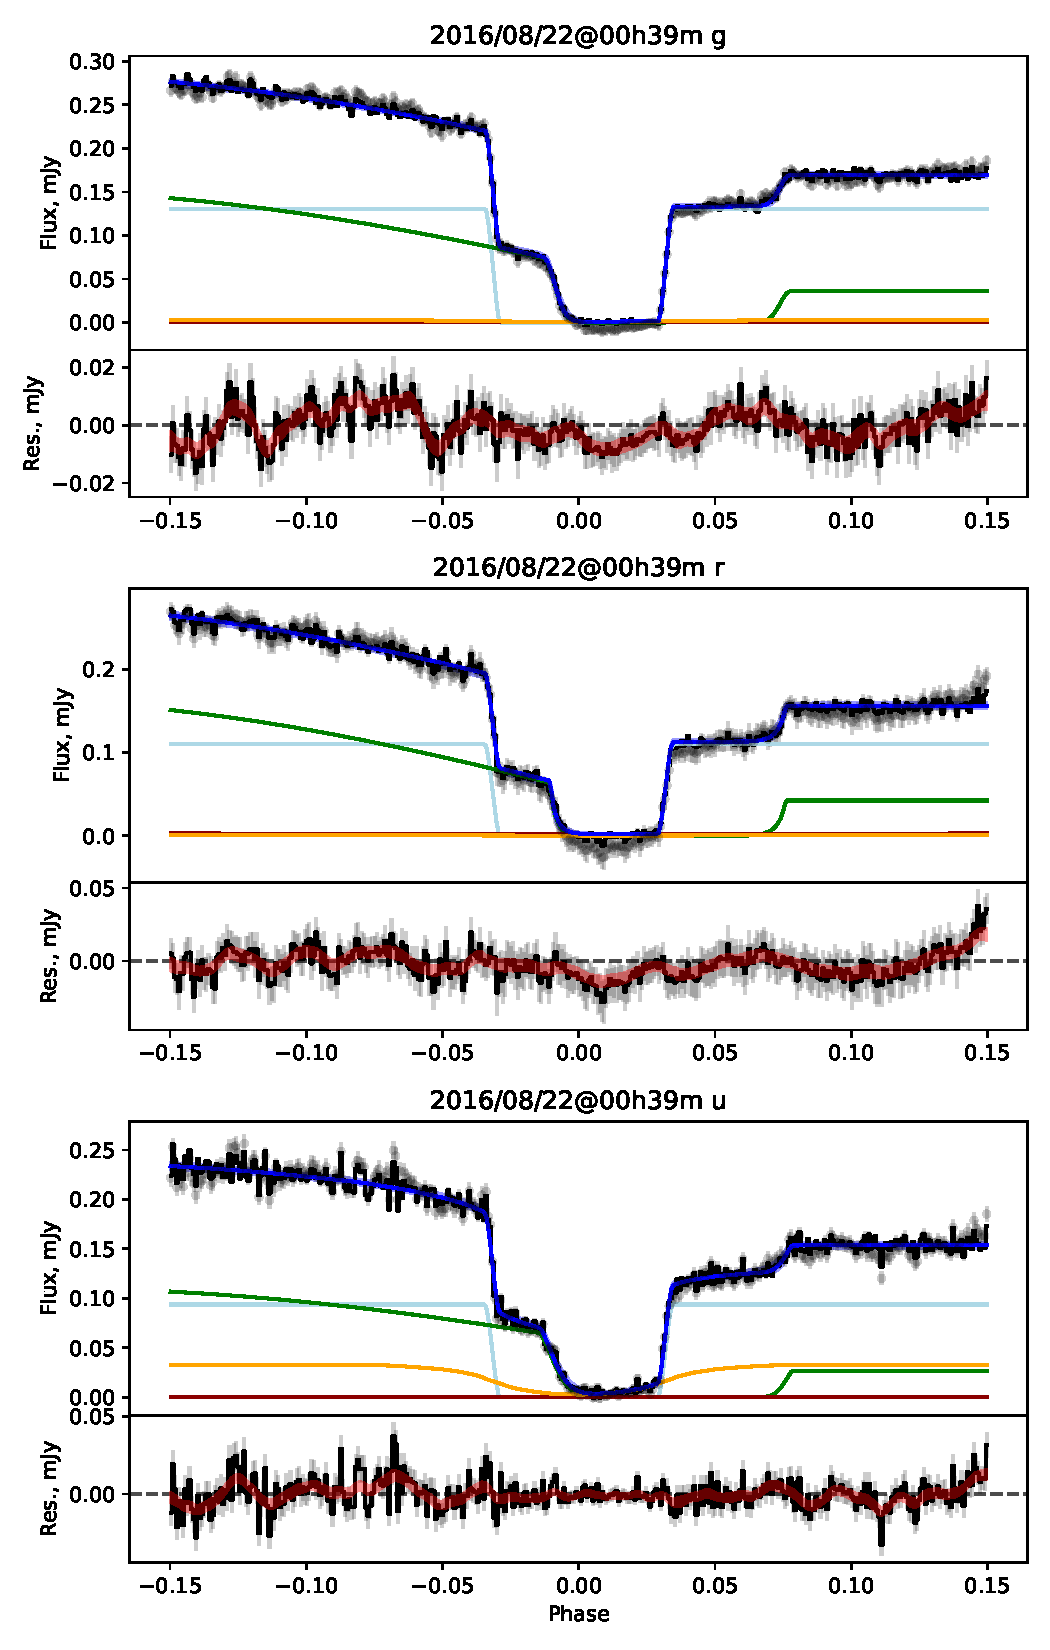
\includegraphics[width=\textwidth]{figures/results/OGLE82/OGLE82_1.pdf}
    \caption{OGLE82 light curve models. Symbols are the same as Figure~\ref{fig:ASASSN-17jf all light curves}}
    \label{fig:OGLE82 all light curves}
\end{figure}
\begin{figure}
    \centering
    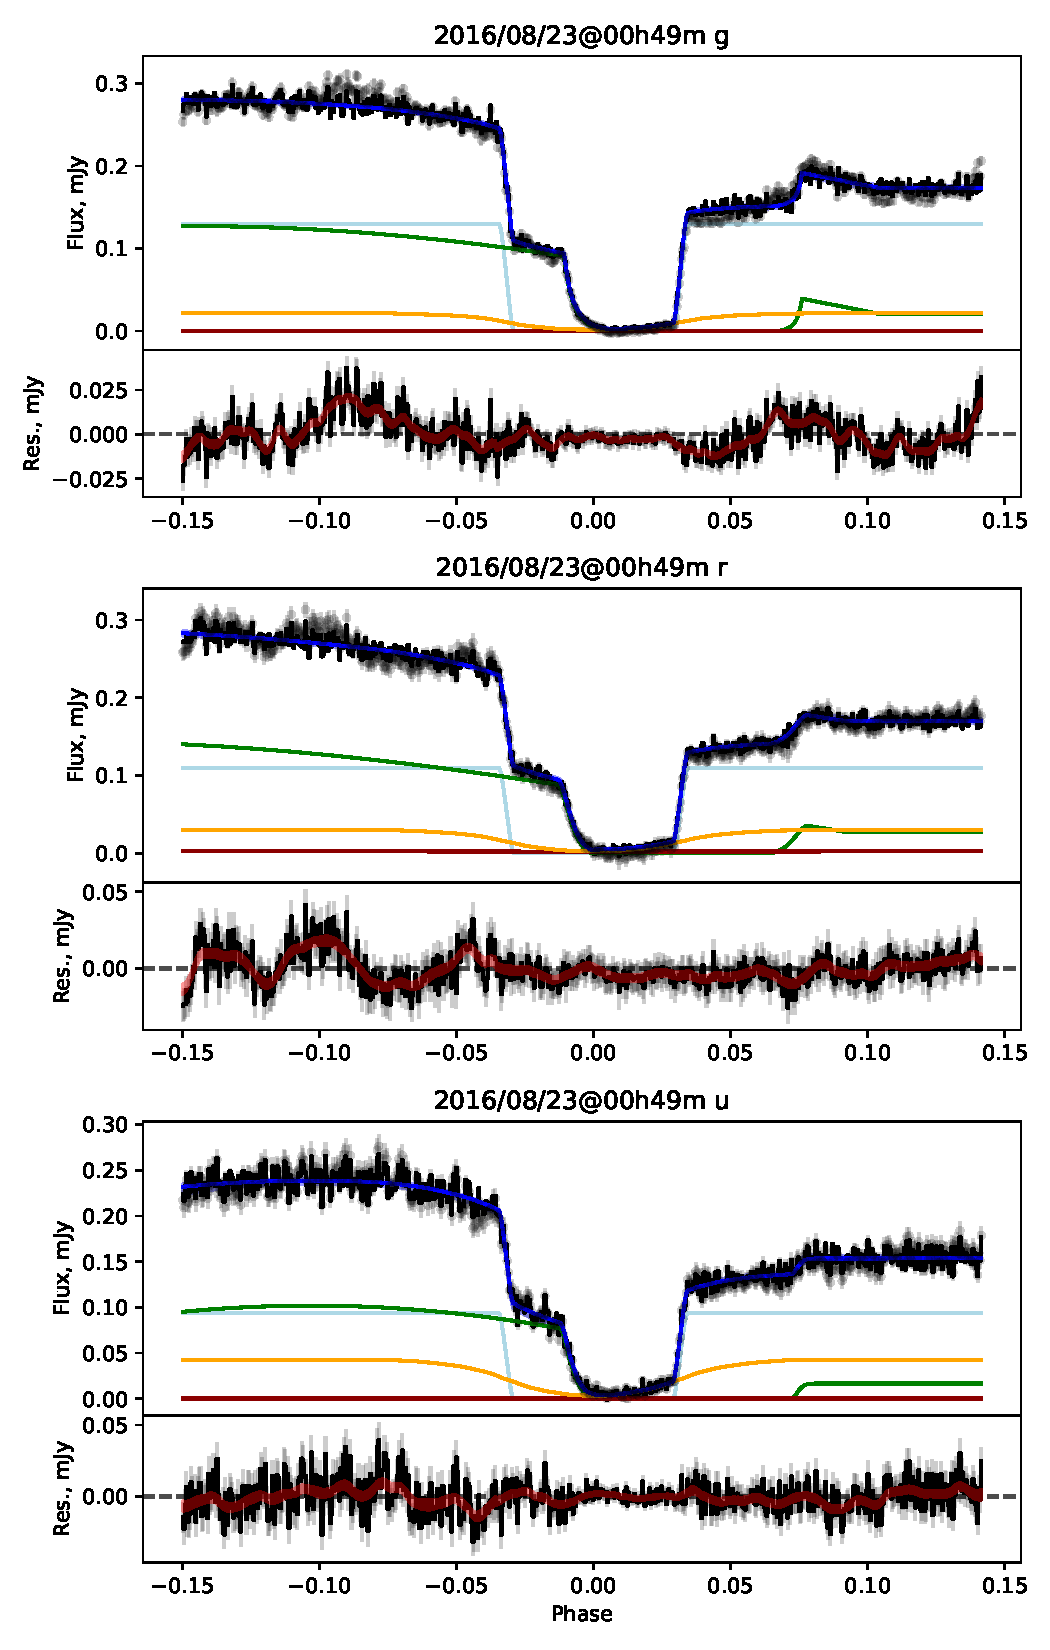
\includegraphics[width=\textwidth]{figures/results/OGLE82/OGLE82_2.pdf}
    \caption{OGLE82 light curve models (cont.)}
    \label{fig:OGLE82 all light curves cont 1}
\end{figure}
\begin{figure}
    \centering
    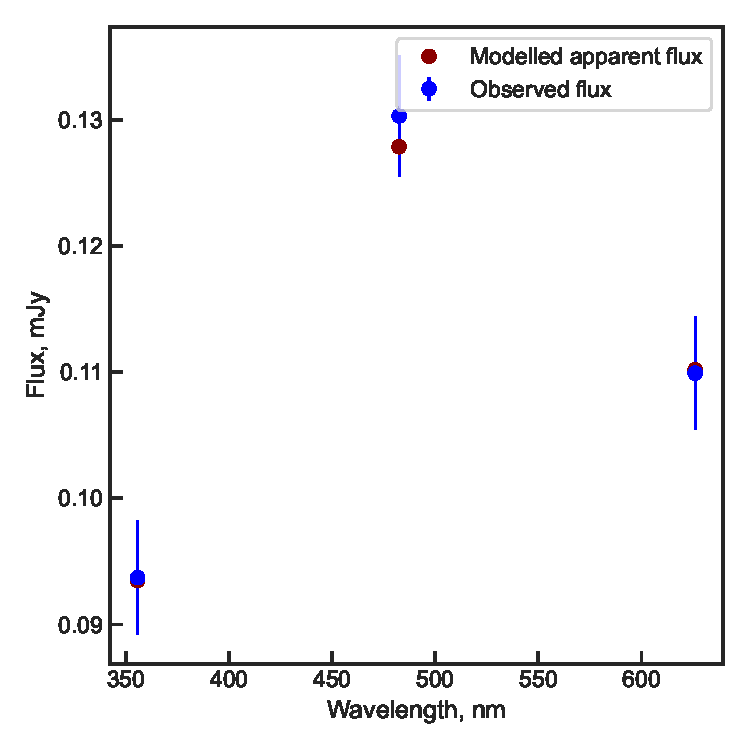
\includegraphics[width=\textwidth]{figures/results/OGLE82/fluxplot.pdf}
    \caption{OGLE82 observed white dwarf fluxes, compared to the best-fit model atmosphere.}
    \label{fig:OGLE82 flux plot}
\end{figure}
\clearpage



\newpage
\subsection{SDSS J0748}

For this system, several KG5 eclipses were recorded over the course of the observations. Whilst it is possible to use KG5 data in modelling, this was not done for this analysis. Rather, the KG5 eclipses were used to constrain the period, then discarded. The KG5 eclipses are still reported in Table~\ref{table:observing:observation logs SDSS0748}.

SDSS J0748 has only two $u'$ band observations, one ULTRACAM observation, and one ULTRASPEC observation. These data have heavily blended white dwarf and bright spot ingresses, which are challenging to model.
The poor $u'$ band data are reflected in the large uncertainty in white dwarf flux, since other important parameters such as $\Delta\phi$ and $R_{\rm wd}$ could be constrained by other eclipses. Importantly, the two eclipses from 2018/2/5 and 2018/2/7 have distinct features, that enable modelling, though interestingly the phase offset between the white dwarf eclipse and bright spot is significant enough that the white dwarf \textit{ingress} is blended with the bright spot \textit{egress} in the case of the former, which is not seen in any other eclipse presented here.


% \begin{landscape}
%     \begin{table}
	\begin{center}
		\caption{Observations taken for SDSS0748.}
		\label{table:observing:observation logs SDSS0748}
		\begin{tabular}{cccccccc}
			\hline
			Instrument & Telescope & Date & Observation start & Observation end & Filter(s) & $T_{\rm ecl}$ & Cycle No. \\
			 &  &  & UTC & UTC &  & BMJD &  \\
			\hline
			\hline
			UCAM  & NTT     & 2017/3/20  & 23:39 & 00:43 & $u_{\rm reg},g_{\rm reg},r_{\rm reg}$ & 57833.00433(3)                                                                                                            &                                         418 \\
			USPEC & TNT     & 2017/1/14  & 20:28 & 20:58 & $KG5$                                 & 57767.87085(2)                                                                                                            &                                        -699 \\
			USPEC & TNT     & 2017/1/17  & 14:14 & 14:42 & $KG5$                                 & 57770.61147(4)                                                                                                            &                                        -652 \\
			USPEC & TNT     & 2017/1/22  & 18:32 & 19:15 & $KG5$                                 & 57775.80116(2)                                                                                                            &                                        -563 \\
			USPEC & TNT     & 2017/2/14  & 12:48 & 13:05 & $KG5$                                 & 57798.54248(2)                                                                                                            &                                        -173 \\
			USPEC & TNT     & 2017/2/14  & 13:55 & 14:27 & $g_{\rm reg}$                         & 57798.60079(3)                                                                                                            &                                        -172 \\
			USPEC & TNT     & 2017/2/15  & 12:24 & 12:54 & $g_{\rm reg}$                         & 57799.53377(3)                                                                                                            &                                        -156 \\
			USPEC & TNT     & 2017/2/24  & 14:11 & 15:20 & $KG5$                                 & 57808.63030(3)                                                                                                            &                                           0 \\
			USPEC & TNT     & 2017/12/12 & 15:20 & 16:01 & $r_{\rm reg}$                         & 58099.66090(2)                                                                                                            &                                        4991 \\
			USPEC & TNT     & 2018/2/1   & 17:21 & 17:53 & $KG5$                                 & 58150.74140(3)                                                                                                            &                                        5867 \\
			USPEC & TNT     & 2018/2/4   & 18:12 & 18:40 & $KG5$                                 & 58153.77358(1)                                                                                                            &                                        5919 \\
			USPEC & TNT     & 2018/2/5   & 17:59 & 18:27 & $r_{\rm reg}$                         & 58154.76487(3)                                                                                                            &                                        5936 \\
			USPEC & TNT     & 2018/2/7   & 15:55 & 16:48 & $r_{\rm reg}$                         & 58156.68913(2)                                                                                                            &                                        5969 \\
			USPEC & TNT     & 2018/12/16 & 22:10 & 22:50 & $g_{\rm reg}$                         & 58468.94496(5)                                                                                                            &                                       11324 \\
			USPEC & TNT     & 2018/12/17 & 16:31 & 16:55 & $g_{\rm reg}$                         & 58469.70301(5)                                                                                                            &                                       11337 \\
			USPEC & TNT     & 2018/12/17 & 19:16 & 19:45 & $r_{\rm reg}$                         & 58469.81963(6)                                                                                                            &                                       11339 \\
			USPEC & TNT     & 2018/12/17 & 20:38 & 21:08 & $KG5$                                 & 58469.87794(5)                                                                                                            &                                       11340 \\
			USPEC & TNT     & 2018/12/17 & 22:04 & 22:37 & $r_{\rm reg}$                         & 58469.93625(4)                                                                                                            &                                       11341 \\
		   \hline
		\end{tabular}
	\end{center}
\end{table}
% \end{landscape}

\begin{figure}
    \centering
    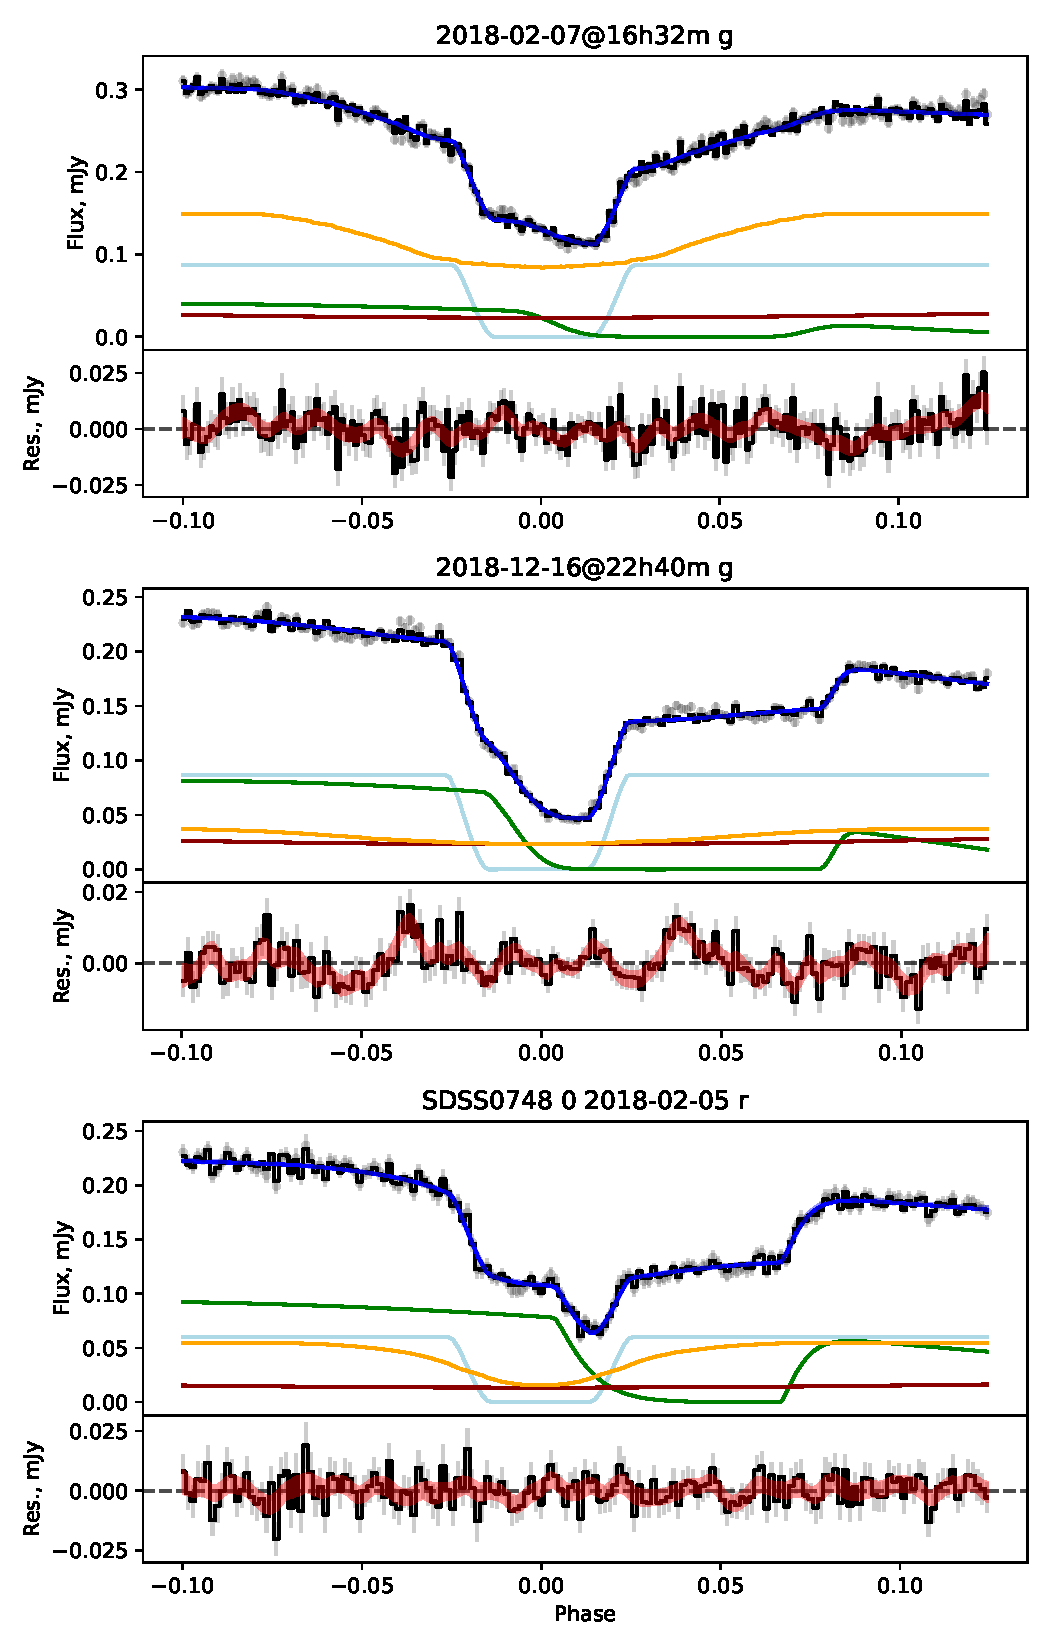
\includegraphics[width=\textwidth]{figures/results/SDSS0748/SDSS0748_1.pdf}
    \caption{SDSS J0748 light curve models. Symbols are the same as Figure~\ref{fig:ASASSN-17jf all light curves}}
    \label{fig:SDSS J0748 all light curves}
\end{figure}
\begin{figure}
    \centering
    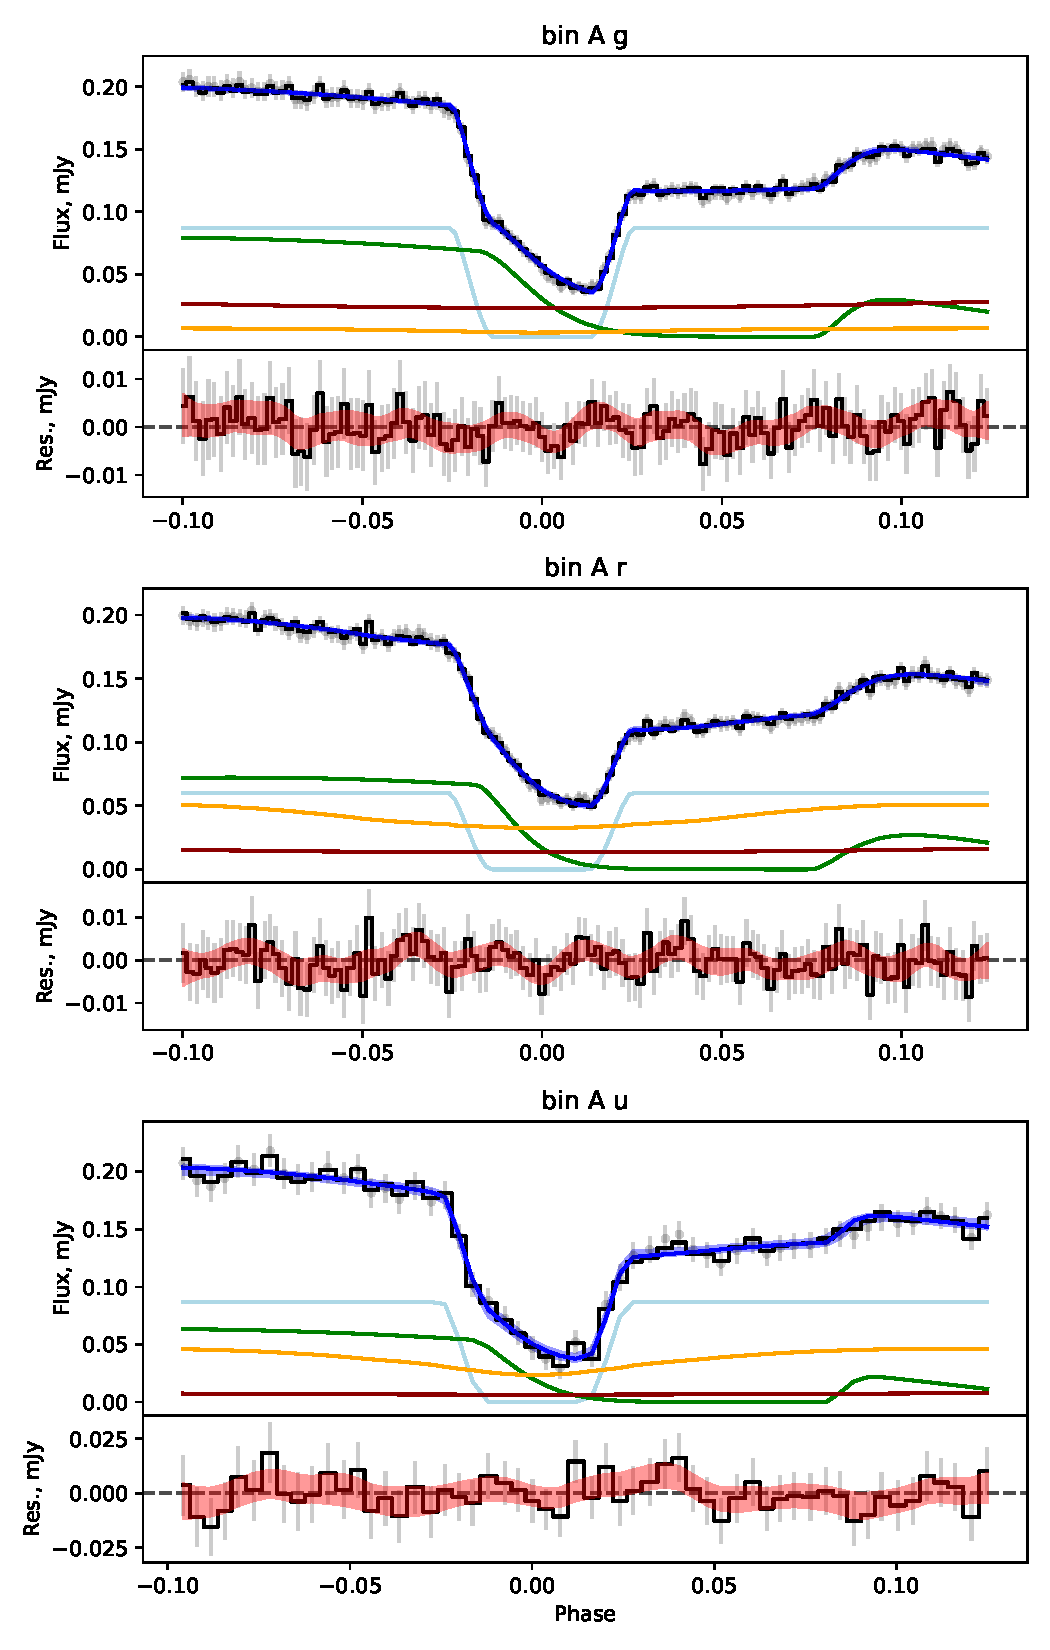
\includegraphics[width=\textwidth]{figures/results/SDSS0748/SDSS0748_2.pdf}
    \caption{SDSS J0748 light curve models (cont.). Data are the result of binning the following eclipses: both eclipses of 2017/2/14, 2017/2/24, 2017/3/20, 2018/12/17.}
    \label{fig:SDSS J0748 all light curves cont 1}
\end{figure}
\begin{figure}
    \centering
    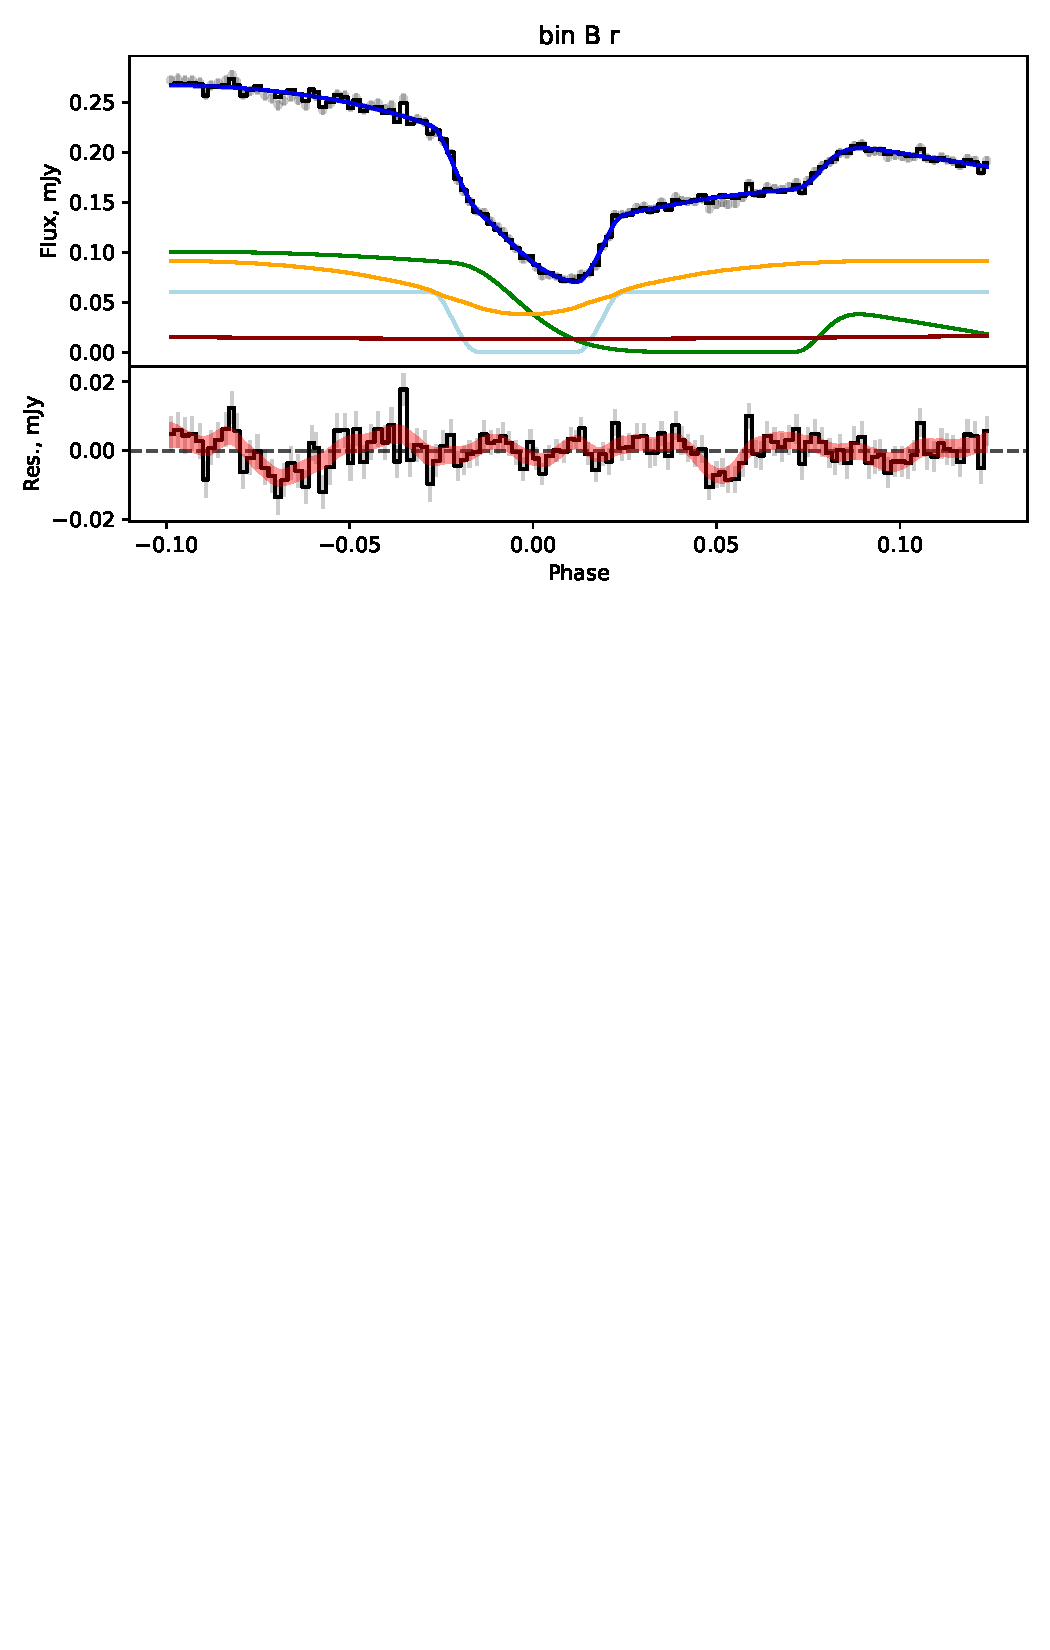
\includegraphics[width=\textwidth, trim={0cm 17cm 0cm 0cm}, clip]{figures/results/SDSS0748/SDSS0748_3.pdf}
    \caption{SDSS J0748 light curve models (cont.). Data are the result of combining the eclipse of 2018/2/4 with the two $r'$ band eclipses observed on 2018/12/17.}
    \label{fig:SDSS J0748 all light curves cont 2}
\end{figure}
\begin{figure}
    \centering
    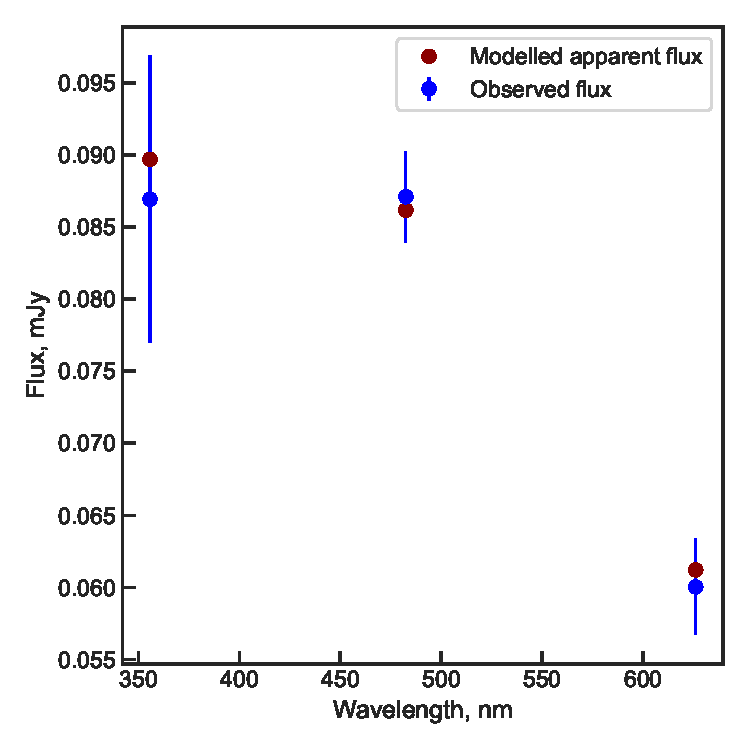
\includegraphics[width=\textwidth]{figures/results/SDSS0748/fluxplot.pdf}
    \caption{SDSS J0748 observed white dwarf fluxes, compared to the best-fit model atmosphere.}
    \label{fig:SDSS0748 flux plot}
\end{figure}
\clearpage



\newpage
\subsection{SDSS J1524}

The binning of this system was somewhat non-standard, as the three filters on the eclipse of 2014/3/3 were not all equally consistent. The $g_{\rm reg}$ eclipse was consistent with the A binning group, but the $u_{\rm reg}$ and $r_{\rm reg}$ eclipses were not.
As such, the $u_{\rm reg}$ and $r_{\rm reg}$ eclipses of this observation were fit individually, and the $g_{\rm reg}$ light curve was binned with the other relevant data.
The resulting fits are broadly satisfactory, though some eclipses (namely the $g_{\rm reg}$ and $r_{\rm reg}$ eclipses of the A binning group) appear to have fairly poor white dwarf ingresses and egresses.
However, the resulting fits give a well-constrained donor mass that agrees strongly with the `optimal' \citet{knigge11} donor track, suggesting the results are reasonable. The white dwarf fits are not ideal, but do not diverge from models by enough to cause concern.




% \begin{landscape}
%     \begin{table}
	\begin{center}
		\caption{Observations taken for SDSS J152419.33+220920.0. Note that the observations showed some color-dependent variability, so were binned with a different grouping.}
		\label{table:observing:observation logs SDSS J152419.33+220920.0}
		\begin{tabular}{ccccccccc}
			\hline
			Instrument & Telescope & Date & Observation  & Observation  & Filter(s) & $T_{\rm ecl}$ & Cycle No. & Binning \\
			 &  &  &  start &  end &  &  &  & ID \\
			 &  &  & TDB & TDB &  & MJD &  &  \\
			\hline
			\hline
			UCAM & NTT & 2011/5/28  & 03:34 & 04:10 & $u_{\rm reg},g_{\rm reg},r_{\rm reg}$ & 55709.16440(1) & -11907 & A \\
			UCAM & NTT & 2011/5/31  & 02:05 & 02:45 & $u_{\rm reg},g_{\rm reg},r_{\rm reg}$ & 55712.10374(1) & -11862 & A \\
			UCAM & NTT & 2011/6/2   & 02:48 & 04:50 & $u_{\rm reg},g_{\rm reg},r_{\rm reg}$ & 55714.12865(1) & -11831 & A \\
			UCAM & WHT & 2012/4/29  & 03:11 & 03:38 & $u_{\rm reg},g_{\rm reg},r_{\rm reg}$ & 56046.14373(1) & -6748  & B \\
			UCAM & WHT & 2012/4/29  & 23:08 & 00:07 & $u_{\rm reg},g_{\rm reg},r_{\rm reg}$ & 56046.99290(1) & -6735  & B \\
			UCAM & WHT & 2013/7/13  & 21:30 & 22:09 & $u_{\rm reg},g_{\rm reg},i_{\rm reg}$ & 56486.91456(1) & 0      & A \\
			UCAM & WHT & 2013/7/21  & 20:49 & 21:30 & $u_{\rm reg},g_{\rm reg},i_{\rm reg}$ & 56494.88342(1) & 122    & A \\
			UCAM & WHT & 2013/7/30  & 21:01 & 21:50 & $u_{\rm reg},g_{\rm reg},i_{\rm reg}$ & 56503.89743(1) & 260    & A \\
			UCAM & WHT & 2013/8/5   & 22:50 & 23:51 & $u_{\rm reg},g_{\rm reg},r_{\rm reg}$ & 56509.97209(1) & 353    & B \\
			UCAM & WHT & 2014/3/3   & 05:47 & 06:23 & $u_{\rm reg},g_{\rm reg},r_{\rm reg}$ & 56719.25331(1) & 3557   & g A, \\
			     &     &            &       &       &                                       &                &        & r \& u fit \\
				 &     &            &       &       &                                       &                &        & individually \\
			UCAM & WHT & 2014/8/2   & 22:58 & 23:39 & $u_{\rm reg},g_{\rm reg},r_{\rm reg}$ & 56871.96768(1) & 5895   & - \\
			% UCAM & WHT & 2014/8/4   & 56873.921 & 56873.937 & $u_{\rm reg},g_{\rm reg},r_{\rm reg}$ & - & 5925   & B \\
		   \hline
		\end{tabular}
	\end{center}
\end{table}
% \end{landscape}

\begin{figure}
    \centering
    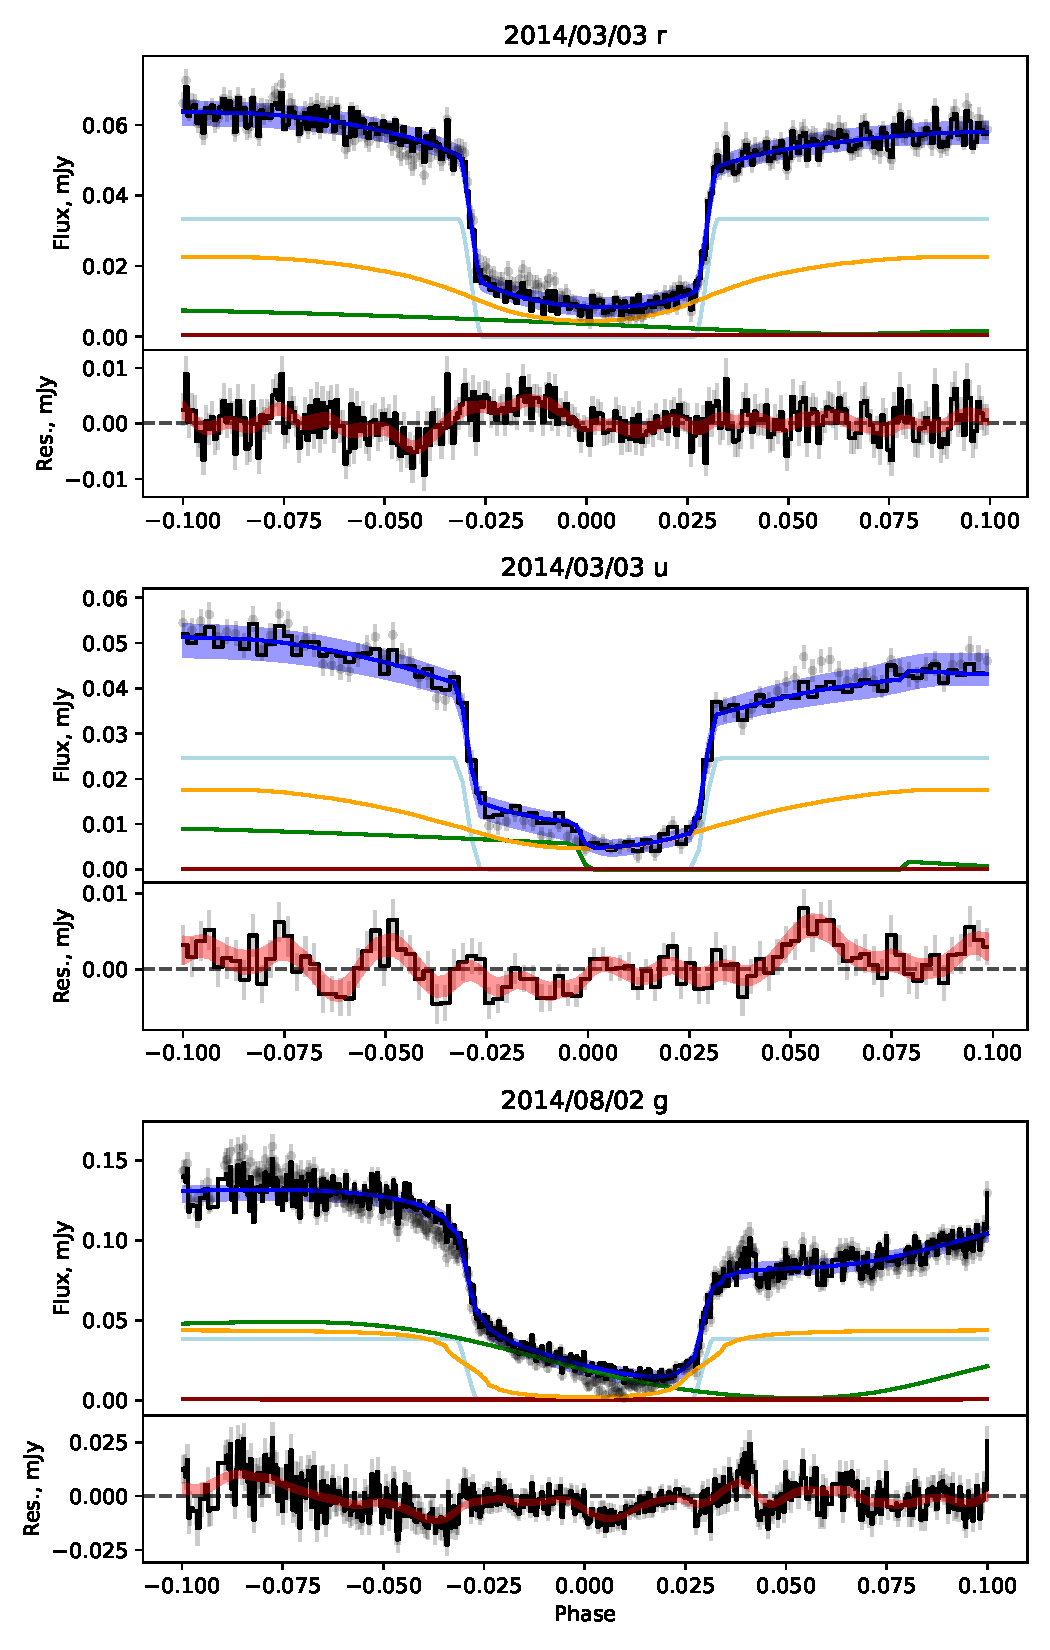
\includegraphics[width=\textwidth]{figures/results/SDSS1524/SDSS1524_1.pdf}
    \caption{SDSS J1524 light curve models. Symbols are the same as Figure~\ref{fig:ASASSN-17jf all light curves}}
    \label{fig:SDSS1524 all light curves}
\end{figure}
\begin{figure}
    \centering
    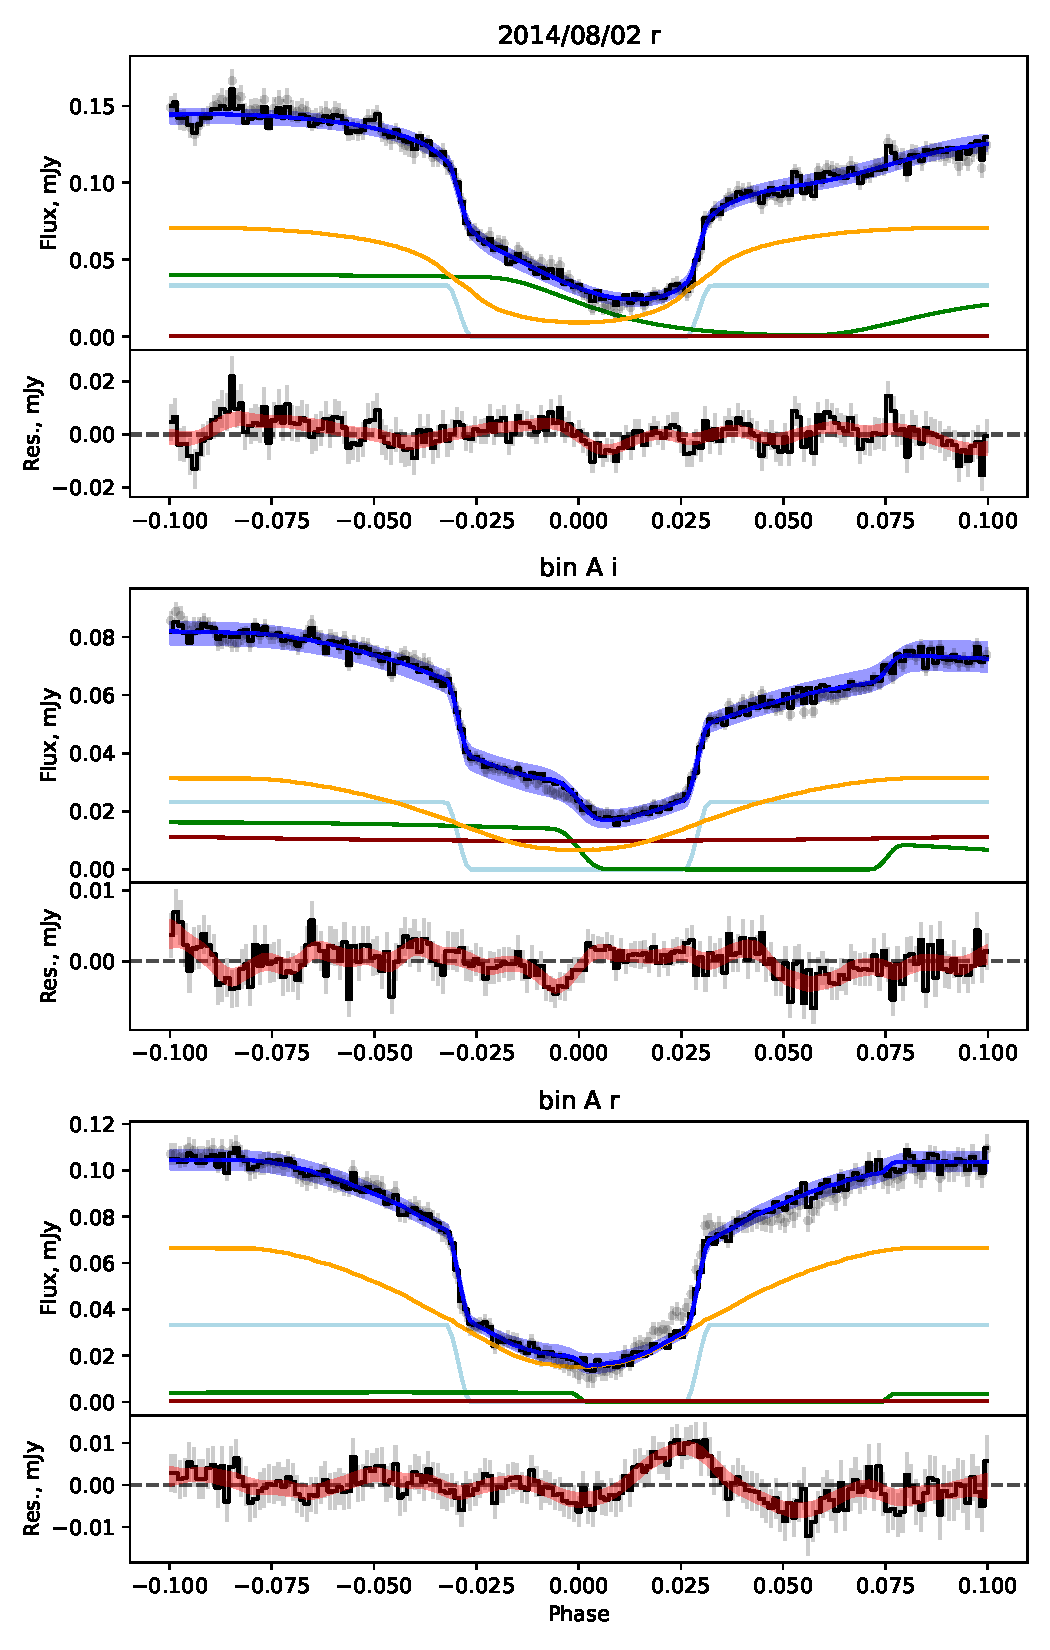
\includegraphics[width=\textwidth]{figures/results/SDSS1524/SDSS1524_2.pdf}
    \caption{SDSS J1524 light curve models (cont.). Binned data are the result of combining eclipses from 2011/5/28, 2011/5/31, 2011/6/2, 2013/7/13, 2013/7/21, 2013/7/30, and, in the case of the $g'$ band, 2014/3/3.}
    \label{fig:SDSS1524 all light curves cont 1}
\end{figure}
\begin{figure}
    \centering
    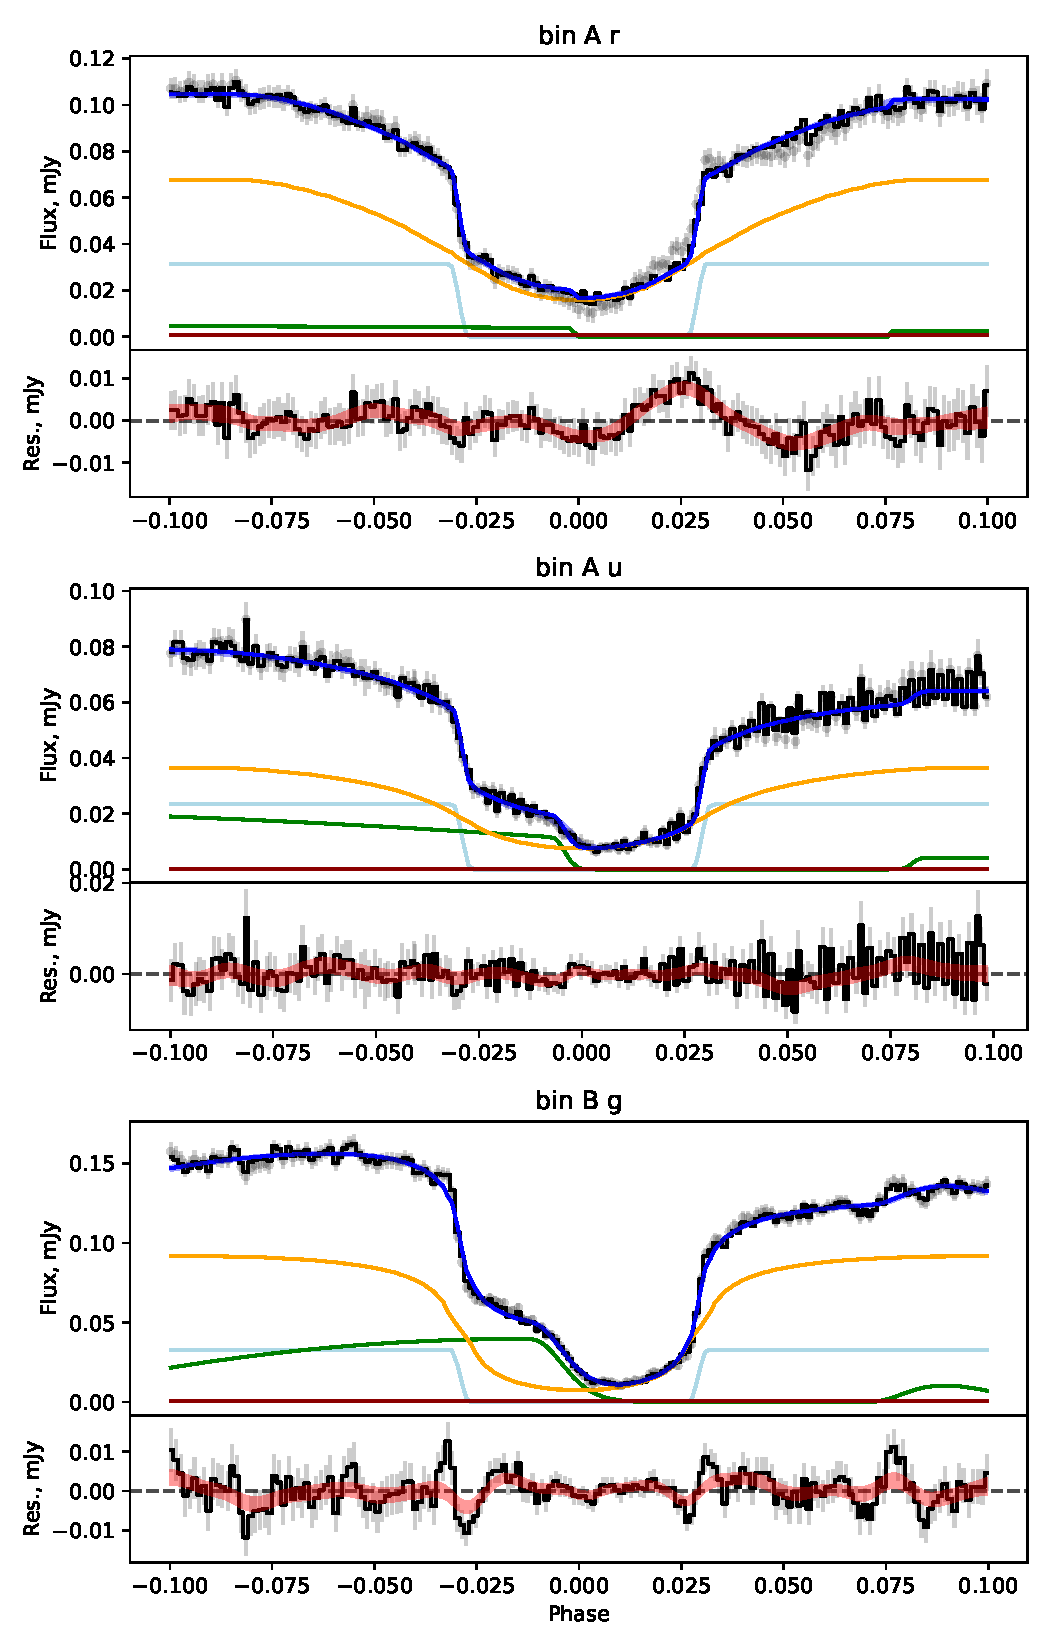
\includegraphics[width=.95\textwidth, trim={0cm 0cm 0cm 0cm}, clip]{figures/results/SDSS1524/SDSS1524_3.pdf}
    \caption{SDSS J1524 light curve models (cont.). Data labelled `bin A' are a combination of the eclipses from the nights of Binned data are the result of combining eclipses from 2011/5/28, 2011/5/31, 2011/6/2, 2013/7/13, 2013/7/21, and 2013/7/30. Data labelled `bin B' are the combination of 2012/4/29, 2012/4/29, and 2013/8/5.}
    \label{fig:SDSS1524 all light curves cont 2}
\end{figure}
\begin{figure}
    \centering
    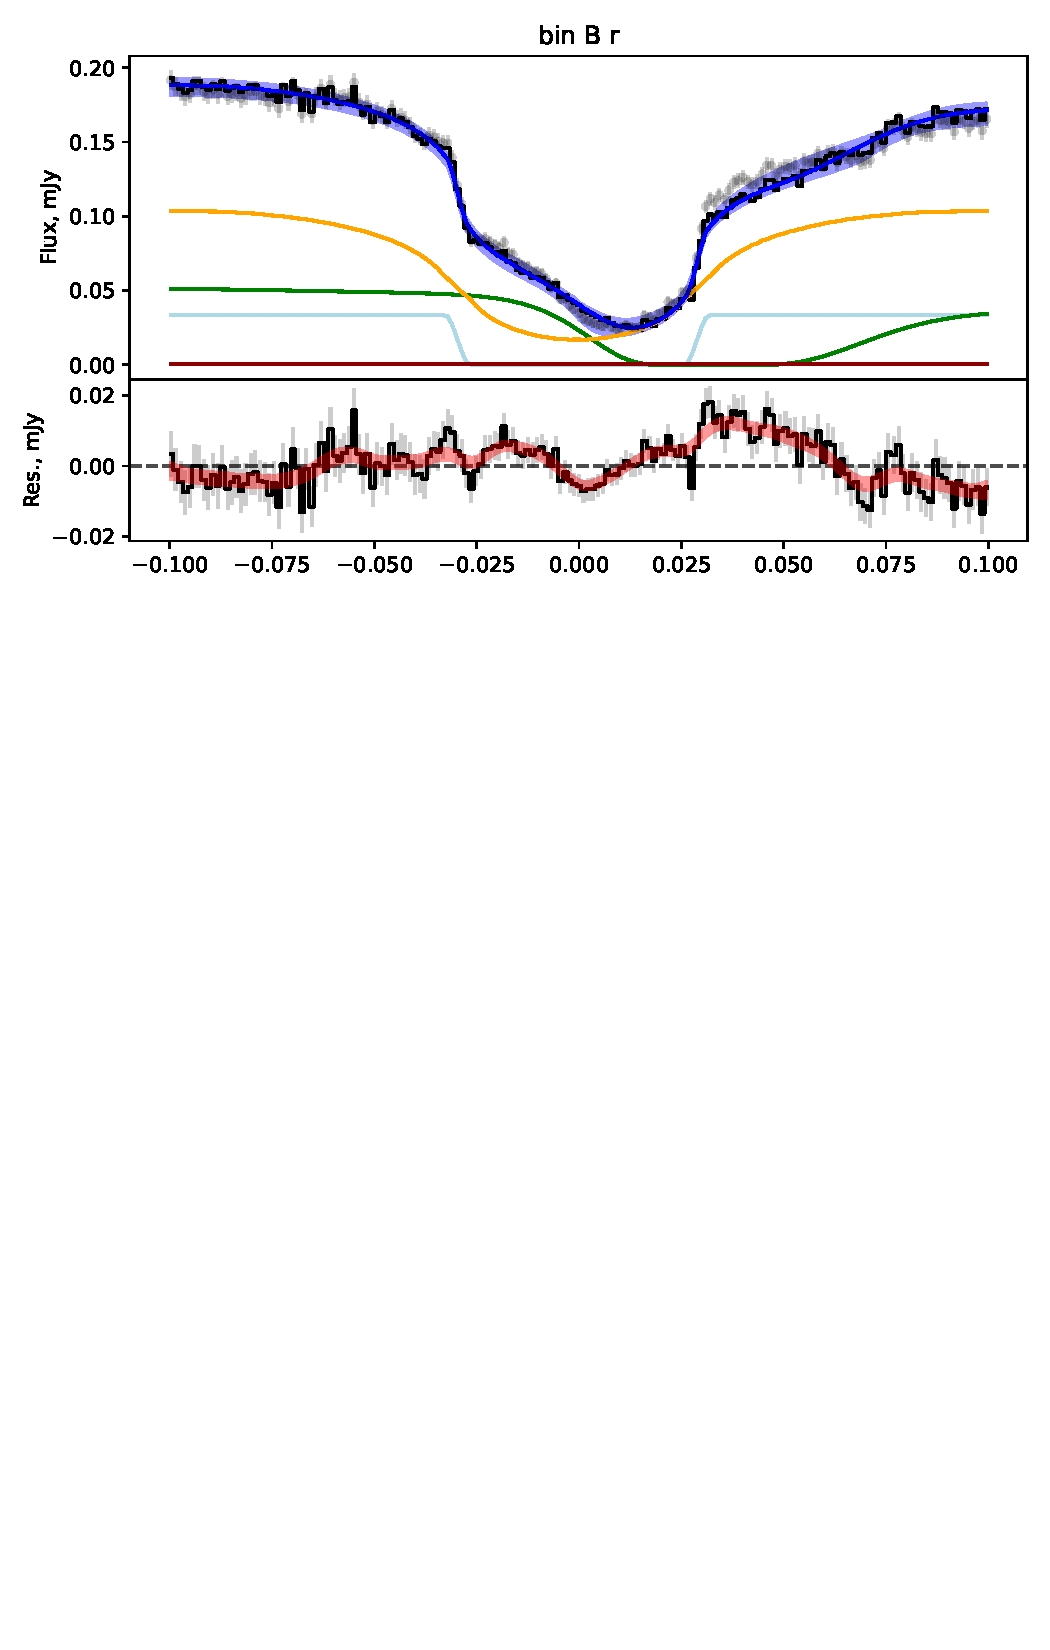
\includegraphics[width=\textwidth, trim={0cm 17cm 0cm 0cm}, clip]{figures/results/SDSS1524/SDSS1524_4.pdf}
    \caption{SDSS J1524 light curve models (cont.). Data are the combination of 2012/4/29, 2012/4/29, and 2013/8/5.}
    \label{fig:SDSS1524 all light curves cont 3}
\end{figure}
\begin{figure}
    \centering
    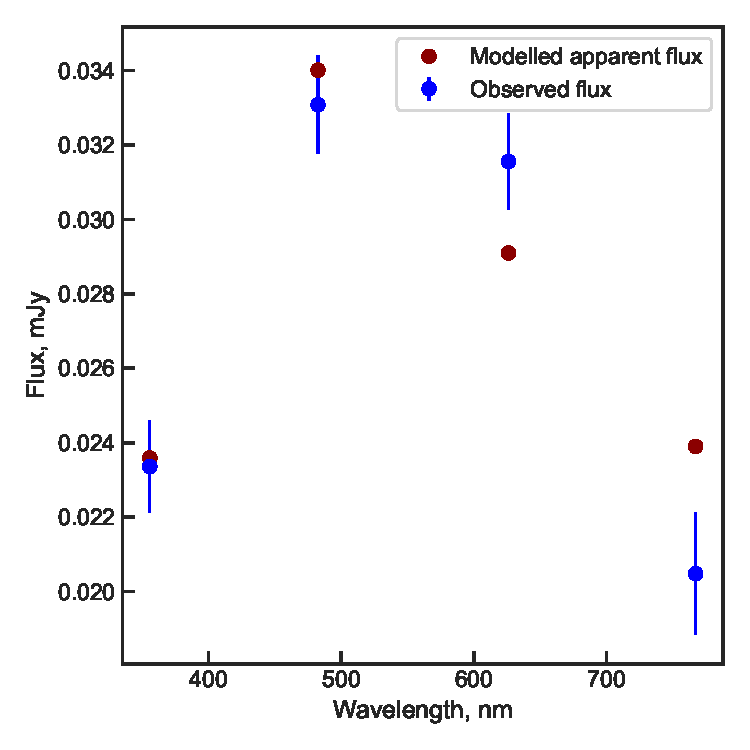
\includegraphics[width=\textwidth]{figures/results/SDSS1524/fluxplot.pdf}
    \caption{SDSS1524 observed white dwarf fluxes, compared to the best-fit model atmosphere.}
    \label{fig:SDSS1524 flux plot}
\end{figure}
\clearpage






\newpage

\begin{table*}
    \centering
    \caption{The system parameters found for the CVs analysed here. The reported parallax, $\pi$, is the posterior distribution from fitting the white dwarf fluxes, c.f.~\S\ref{sect:modelling:fitting white dwarf colours}.}
    \label{table:12 new cvs:system_parameters}
    \begin{tabular}{cccc}
        \hline
        \textbf{System Name:}      & \textbf{ASASSN-14hq}    & \textbf{ASASSN-14kb}     & \textbf{ASASSN-15pb}  \\
        \hline
        \hline
        $M_\mathrm{wd}/M_\odot$    & $0.67\pm0.01$           & $0.74\pm0.02$            & $0.72\pm0.03$         \\
        $R_\mathrm{wd}/R_\odot$    & $0.0119\pm0.0001$       & $0.0113\pm0.0002$        & $0.0115\pm0.0005$     \\
        $M_\mathrm{donor}/M_\odot$ & $0.097\pm0.002$         & $0.134\pm0.003$          & $0.148\pm0.008$       \\
        $R_\mathrm{donor}/R_\odot$ & $0.157\pm0.001$         & $0.164\pm0.001$          & $0.210\pm0.004$       \\
        $q$                        & $0.145\pm0.002$         & $0.182\pm0.002$          & $0.206\pm0.004$       \\
        \hline
        $P$, hours                 & $1.78384800(7)$         & $1.63453(1)$             & $2.23896(3)$          \\
        $a/R_\odot$                & $0.681\pm0.004$         & $0.670\pm0.005$          & $0.824\pm0.014$       \\
        $i$                        & $80.35\pm0.06$          & $84.4\pm0.1$             & $79.4\pm0.1$          \\
        $K_\mathrm{wd}$, km/s      & $58.0\pm0.9$            & $76.2\pm1$               & $75\pm2$              \\
        $K_\mathrm{donor}$, km/s   & $399\pm2$               & $419\pm3$                & $364\pm6$             \\
        \hline
        $\pi$, mas                 & $3.40\pm0.07$           & $2.78\pm0.11$            & $1.0\pm0.2$           \\
        $T_{\rm eff}$, K           & $14819\pm800$           & $17700\pm1000$           & $19200\pm1600$        \\
        $\log(g), {\rm cgs}$       & $8.11\pm0.02$           & $8.21\pm0.03$            & $8.17\pm0.06$         \\
        \hline
        \hline \\[2em]
        \hline
        \textbf{System Name:}      & \textbf{ASASSN-17fo}      & \textbf{AY For}        & \textbf{CSS090102}     \\
        \hline \hline \\
        $M_\mathrm{wd}/M_\odot$    & $0.85\pm0.01$             & $0.78\pm0.02$          & $0.62\pm0.03$          \\
        $R_\mathrm{wd}/R_\odot$    & $0.0099\pm0.0001$         & $0.0106\pm0.0003$      & $0.0126\pm0.0004$      \\
        $M_\mathrm{donor}/M_\odot$ & $0.109\pm0.002$           & $0.106\pm0.006$        & $0.060\pm0.003$        \\
        $R_\mathrm{donor}/R_\odot$ & $0.1436\pm0.0007$         & $0.162\pm0.003$        & $0.119\pm0.002$        \\
        $q$                        & $0.1267\pm0.0005$         & $0.136\pm0.004$        & $0.094\pm0.002$        \\
        \hline
        $P$, hours                 & $1.477147(2)$             & $1.790756(1)$          & $1.49723786(5)$        \\
        $a/R_\odot$                & $0.646\pm0.003$           & $0.717\pm0.007$        & $0.582\pm0.008$        \\
        $i$                        & $84.23\pm0.03$            & $84.0\pm0.2$           & $88.7\pm0.6$           \\
        $K_\mathrm{wd}$, km/s      & $60.2\pm0.4$              & $57.8\pm2.0$           & $40.9\pm1.2$           \\
        $K_\mathrm{donor}$, km/s   & $468\pm2$                 & $425\pm4$              & $431\pm6$              \\
        \hline
        $\pi$, mas                 & $1.79\pm0.36$             & $2.12\pm0.16$          & $1.41\pm0.30$          \\
        $T_{\rm eff}$, K           & $14800\pm600$             & $18100\pm500$          & $14800\pm1200$         \\
        $\log(g), {\rm cgs}$       & $8.37\pm0.02$             & $8.28\pm0.04$          & $8.00\pm0.33$          \\
        \hline
        \hline \\[2em]
    \end{tabular}
\end{table*}

\begin{table*}
    \centering
    \caption{Table~\ref{table:12 new cvs:system_parameters}, continued.}
    \label{table:12 new cvs:system_parameters cont 1}
    \begin{tabular}{cccc}
        \hline
        \textbf{System Name:}      & \textbf{CSS090419}     & \textbf{CSS090622}    & \textbf{MASOT0014}     \\
        \hline \hline \\
        $M_\mathrm{wd}/M_\odot$    & $0.59\pm0.08$          & $0.67\pm0.06$         & $0.86\pm0.03$          \\
        $R_\mathrm{wd}/R_\odot$    & $0.0122\pm0.0009$      & $0.0112\pm0.0007$     & $0.0097\pm0.0003$      \\
        $M_\mathrm{donor}/M_\odot$ & $0.087\pm0.011$        & $0.104\pm0.009$       & $0.122\pm0.007$        \\
        $R_\mathrm{donor}/R_\odot$ & $0.152\pm0.007$        & $0.155\pm0.005$       & $0.165\pm0.003$        \\
        $q$                        & $0.146\pm0.003$        & $0.159\pm0.008$       & $0.142\pm0.004$        \\
        \hline
        $P$, hours                 & $1.81062621(6)$        & $1.702302(6)$         & $1.7167077(5)$         \\
        $a/R_\odot$                & $0.660\pm0.030$        & $0.661\pm0.020$       & $0.722\pm0.008$        \\
        $i$                        & $80.9\pm0.1$           & $88.2\pm0.6$          & $84.8\pm0.3$           \\
        $K_\mathrm{wd}$, km/s      & $56.0\pm2.7$           & $63.7\pm2.5$          & $63.2\pm2.0$           \\
        $K_\mathrm{donor}$, km/s   & $381\pm16$             & $408\pm12$            & $445\pm5$              \\
        \hline
        $\pi$, mas                 & $1.42\pm0.69$          & $2.02\pm0.27$         & $2.42\pm0.11$          \\
        $T_{\rm eff}$, K           & $18200\pm9000$         & $9800\pm1500$         & $17300\pm1000$         \\
        $\log(g), {\rm cgs}$       & $8.04\pm0.12$          & $8.16\pm0.08$         & $8.37\pm0.04$          \\
        \hline
        \hline \\[2em]
        \hline
        \textbf{System Name:}       & \textbf{OGLE82}   & \textbf{SDSS J0748}    & \textbf{SDSS J1524}     \\
        \hline \hline \\
        $M_\mathrm{wd}/M_\odot$     & $0.83\pm0.01$     & $0.68\pm0.02$          & $0.99\pm0.01$           \\
        $R_\mathrm{wd}/R_\odot$     & $0.0099\pm0.0002$ & $0.0121\pm0.0004$      & $0.0082\pm0.0003$       \\
        $M_\mathrm{donor}/M_\odot$  & $0.131\pm0.004$   & $0.066\pm0.004$        & $0.097\pm0.003$         \\
        $R_\mathrm{donor}/R_\odot$  & $0.170\pm0.002$   & $0.117\pm0.002$        & $0.144\pm0.001$         \\
        $q$                         & $0.157\pm0.002$   & $0.095\pm0.004$        & $0.099\pm0.001$         \\
        \hline
        $P$, hours                  & $1.7263398(6)$    & $1.39947(1)$           & $1.56764953(2)$         \\
        $a/R_\odot$,                & $0.720\pm0.006$   & $0.575\pm0.007$        & $0.701\pm0.006$       \\
        $i$                         & $83.9\pm0.1$      & $81.7\pm0.2$           & $85.8\pm0.1$            \\
        $K_\mathrm{wd}$, km/s       & $68.5\pm1.0$      & $42.2\pm1.8$           & $48.6\pm0.8$            \\
        $K_\mathrm{donor}$, km/s    & $435\pm3$         & $450\pm5$              & $493\pm5$               \\
        \hline
        $\pi$, mas                  & $3.82\pm0.12$     & $1.83\pm0.14$          & $1.95\pm0.18$           \\
        $T_{\rm eff}$, K            & $18000\pm4000$    & $22500\pm3000$         & $12500\pm900$          \\
        $\log(g), {\rm cgs}$        & $8.37\pm0.03$     & $8.11\pm0.03$          & $8.61\pm0.04$           \\
        \hline
        \hline
    \end{tabular}
\end{table*}



\section{Comparing observations with model donor tracks}
\label{sect:12 new cvs:eclipse modelling of 12 CVs}

The observed donor properties can be compared to the \citet{knigge11}-like MESA donor tracks. Figure~\ref{fig:12 new cvs:donor model with eclipsers plotted} shows the full sample of short-period eclipse modelled CVs (a catalogue of these systems is given in Appendix~\ref{appendix:eclipse modelled CV data tables}) plotted with the `standard' donor track that includes only gravitational braking below the gap and the disagreement between model and data indeed persists.

There is a large scatter in the observations, but new data continue to lie systematically to the right of the `standard' model track (shown by the blue line), and the need for extra AML continues to be supported by observations.
The new data appear to have a significant scatter about the canonical donor evolutionary tracks.
Typically, scatter in CV donor tracks is explained as being due to different white dwarf masses, but the effect of this on $P$ is thought to be relatively small, on the order of a few minutes \citep{goliasch2015}, and falls significantly short of explaining these new results.
Further discrediting this as the source of scatter is Figure~\ref{fig:12 new cvs:donor model with eclipsers plotted}, which illustrates that whilst the average white dwarf mass of this sample is indeed slightly lower than the canonical \citet{pala2020} value, the difference is small and its effects are unlikely to be significant.

There are then two possibilities for this scatter: either the parameter estimations of this thesis are somehow flawed, or CV donor evolution is not as unified as believed; at this time, it is difficult to rule out either option.
The majority of the eclipse model fits do not give significant cause for concern about their validity. In theory, the new hierarchical model only requires a single example of distinct egresses to constrain the mass ratio, with other eclipses only needed to constrain the white dwarf fluxes. However, I have not included a thorough study into the hierarchical model's ability to recover parameters from blended eclipse features. Such a study would be desirable, to better understand the capabilities of the new model.
If, however, these results are to be believed (and there is little cause not to), this may indicate that the canonical idea of a unified track does not account for possibly significant effects, such as variation in the age or formation metallicity of the donor, or variations in the degree of excess AML that is known to be present in these CVs.


% \todo{The K11 mass-radius relation could be updated? Not really worth it, not my focus and not that many new systems.}
\begin{figure}
    \centering
    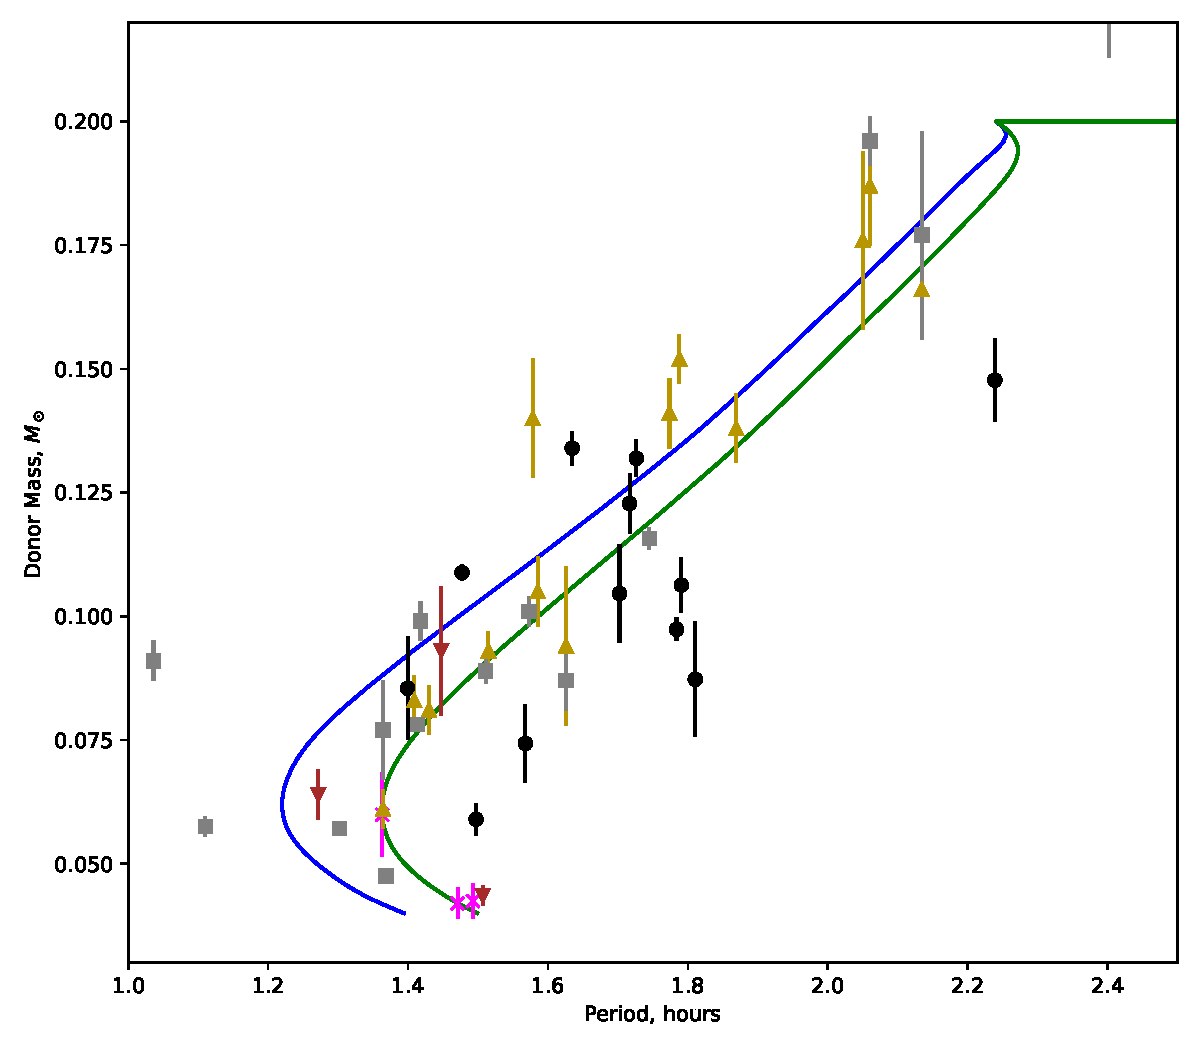
\includegraphics[width=\textwidth]{figures/results/K11_donor_track_with_eclipse_modelled_data.pdf}
    \caption{Showing how eclipse modelled observations compare with evolutionary models in the short period regime. The {\bf solid blue line} is the `standard' \citet{knigge11} donor track with only gravitational braking below the period gap, and the {\bf solid green line} is the `optimal' track with $2.47\times$ amplified gravitational braking. Data points are scaled based on their white dwarf masses. The {\bf magenta crosses} are the 3 CVs with peculiar colours from Chapter~\ref{chpt:three peculiar white dwarfs}, {\bf black circles} are the 12 systems of Chapter~\ref{chpt:characterisation of 12 new CVs}, {\bf gold upright triangles} are data from \citet{McAllister2019}, {\bf grey squares} are from \citet{Savoury2011}, and the {\bf brown inverted triangles} are the supplementary systems from \citet{copperwheat2010,mcallister2015,mcallister2017,mcallister2017b}.}
    \label{fig:12 new cvs:donor model with eclipsers plotted}
\end{figure}

\begin{figure}
    \centering
    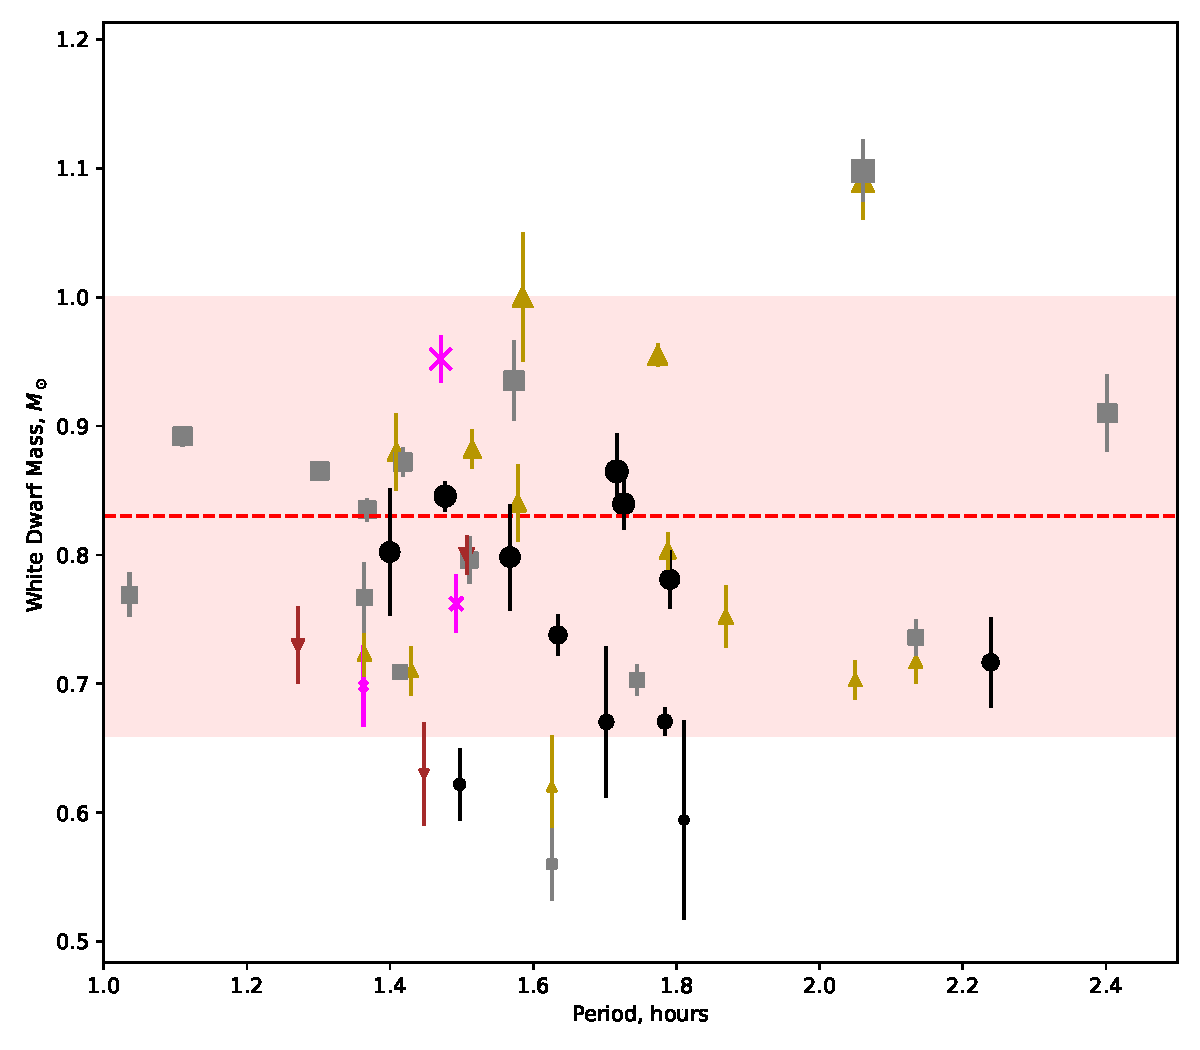
\includegraphics[width=\textwidth]{figures/results/Modelled_Mwd_vs_Period.pdf}
    \caption{Showing how the modelled observations compare with the average white dwarf mass found by \citet{pala2020}, $0.83\pm0.17 M_\odot$, which is shown by the {\bf red dashed line} and {\bf red shaded area}. Data symbols are similar to Figure~\ref{fig:12 new cvs:donor model with eclipsers plotted}, and the data points are similarly scaled to aid understanding of the correlation between datum size and $M_{\rm wd}$.}
    \label{fig:12 new cvs:white dwarf masses vs period}
\end{figure}



\subsection{A preliminary look at AML in CVs}
\label{sect:12 new cvs:period excess}

The published results and analysis of the three CVs in Chapter~\ref{chpt:three peculiar white dwarfs} \citep{wild2021} pre-date the more fully developed method to infer a donor mass loss rate described in \S\ref{sect:modelling:optimising mass loss rate to observations}. However, that preliminary analysis remains of interest, and motivates Chapter~\ref{chpt:Mass loss and Angular momentum loss in short period CVs}.
As such, the preliminary AML analysis method of \citet{wild2021} was repeated using the new data presented here, significantly increasing the population of well-characterised CVs compared to what was available at publication. The core findings of that work persist with the new data set, lending further credence to the results.

In order to qualitatively evaluate missing AML, the period \textit{excess} was examined, $P_{\rm ex} = P_{\rm obs} - P_{\rm std}$. Here, $P_{\rm obs}$ is the observed period, and $P_{\rm std}$ is the period predicted by the \citet{knigge11} CV donor track with only $1\times$ gravitational braking below the period gap, interpolated across $M_{\rm donor}$.
To determine $P_{\rm ex}$ from a measured $(P_{\rm obs}, M_{\rm donor})$ pair, mass samples are drawn from the modelled posterior distribution of $M_{\rm donor}$, and period is interpolated at each mass from the evolutionary tracks to give a corresponding $P_{\rm std}$ distribution. As $P_{\rm std}$ is very sensitive to $M_{\rm donor}$, the $P_{\rm std}$ error dominates the uncertainty in $P_{\rm ex}$.
A positive $P_{\rm ex}$ indicates that the model is missing AML, and a negative $P_{\rm ex}$ indicates a model that has too much AML, relative to an observation.
The validity of $P_{\rm ex}$ is vulnerable to two key systematic biases; the validity of $P_{\rm std}$ (itself contingent on the accuracy of a variety of model assumptions and biases), and the inherent physical variation of the CV population.
% This is the secondary motivation for the development of the more rigorous methodology of \S\ref{sect:modelling:optimising mass loss rate to observations}, after the primary motivation of trying to improve on the qualitative nature of the $P_{\rm ex}$ approach.

CVs may follow inherently different evolutionary tracks due to differences in donor metallicity \citep{stehle1997, harrison2016}, white dwarf mass \citep{knigge2006}, and the age of the donor when it first contacts the Roche lobe \citep{howell2001}. A population-wide scatter in this parameter space is not captured in the \citet{knigge11} model, which uses fixed values for these variables, but justification for the adopted values are given \citep{knigge11, knigge2006}.
If any individual system deviates from the adopted values in the models of \citet{knigge11} then $P_{\rm ex}$ for that system will be influenced by these differences as well as any extra AML. However, conclusions about $P_{\rm ex}$ drawn from the population at large should remain robust, as long as the population doesn't differ systematically from the values adopted in the models.
The white dwarf mass used by \citet{knigge11} is somewhat lower than more recent observations suggest, using $M_{\rm wd} = 0.75 M_\odot$ versus the more recent value of $M_{\rm wd} = 0.83 \pm 0.17 M_\odot$ \citep{pala2020}.
An updated version of Knigge's modelling is necessary to properly characterise the effect of this change on the donor evolutionary tracks, as this will affect both the size of the Roche lobes, and the rate of gravitational wave AML.
Other CV models suggest that the effect of correcting $M_{\rm wd}$ will be small, at most around 2 minutes \citep{goliasch2015}. This analysis is not rigorous enough for this to become an issue, and the effects of using an incorrect white dwarf mass is considered acceptable.

More seriously, $P_{\rm ex}$ is only an accurate proxy of additional AML if the underlying donor physics in the model are correct. For example, if the models incorrectly predict the mass of systems in the period gap, this can have a large effect on $P_{\rm ex}$. In the models of \citet{knigge11} this mass is fixed at the empirically derived value of $0.2 M_\odot$, as observations of superhumping and eclipsing CVs suggest that period gap occurs at donor masses of $0.20 \pm 0.02 M_\odot$ \citep{knigge2006}. Using model tracks with lower or higher masses for the donor mass of the period gap would alter $P_{\rm ex}$, though in this case the broad trend in $P_{\rm ex}$ will again be unchanged.

The result is plotted in Figure~\ref{fig:period excess}. These data are fit with a straight line, and as the data have significant uncertainty in both axes, the sum orthogonal distance (weighted by uncertainty) from the data is minimised to find the best fit \citep{hogg2010}. Python's \lstinline{SciPy} package, \lstinline{ODR} was used to perform this fitting.

 The best-fit lines to the two data sets are $P_{\rm ex} / \mathrm{hours} = -(4.07\pm0.83) M_{\rm donor}/M_\odot + (0.32\pm0.06)$ and $P_{\rm ex} / \mathrm{hours} = -(1.62\pm0.27) M_{\rm wd}/M_\odot + (1.34\pm0.21)$.
The best-fit slope of $P_{\rm ex}$ as a function of both $M_{\rm donor}$ and $M_{\rm wd}$ is significantly correlated: $5\sigma$ from the null hypothesis of 0 in the case of $M_{\rm wd}$, and $\sim 3\sigma$ for $M_{\rm donor}$.
 However, note that the best-fit line for $M_{\rm donor}$ does \textit{not} pass through $P_{\rm ex} = 0$ at $M_{\rm donor} = 0.20 M_\odot$ as expected, unless $>3\sigma$ confidence on the gradient and intercept are considered.

Again, it is stressed that the only robust product of this analysis is the \textit{sign of the gradient} of the $M - P_{\rm ex}$ relationship, and that its steepness and y-intercept are both subject to systematic errors that are not captured in the statistical errors given above. Despite this, the clear and statistically significant increase in $P_{\rm ex}$ towards low masses implies that additional AML has a larger effect on the donor at lower component masses.

Note that $P_{\rm ex}$ considers a changing gravitational braking strength, which declines as the total system mass falls.
There are then three cases to describe the trend in $P_{\rm ex}$: the excess AML also declines in strength but more slowly than gravitational losses; excess AML is roughly constant across the range of $M_{\rm donor}$ or $M_{\rm wd}$; or excess AML actually increases in strength towards lower $M_{\rm donor}$ or $M_{\rm wd}$. Note that none of these options translate to the ``optimal'' \citet{knigge11} models which adopt additional AML of the same form as GWB, but are compatible with the eCAML solution for excess AML.


\begin{figure}
    \centering
    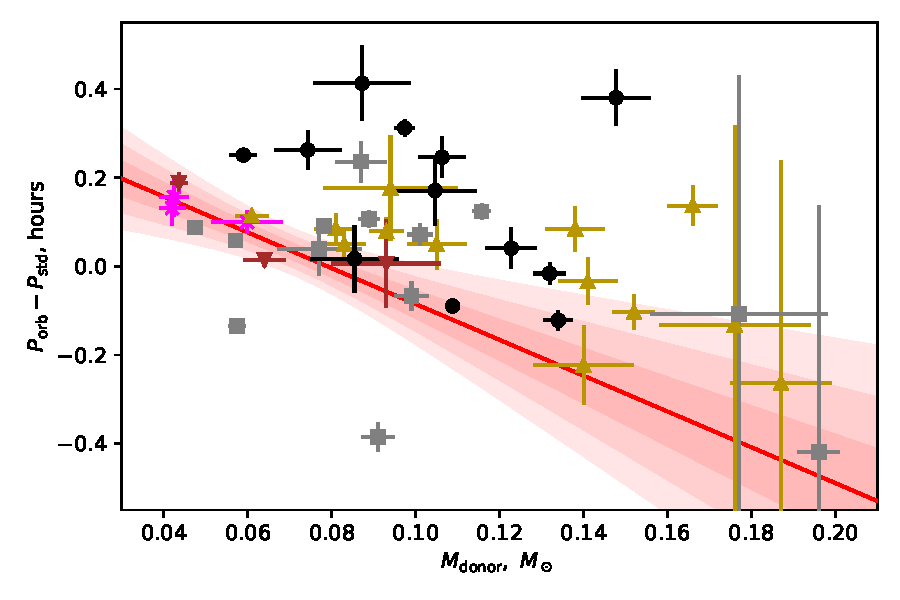
\includegraphics[width=\columnwidth]{figures/results/Mdot/Period_excess_Mr.pdf}
    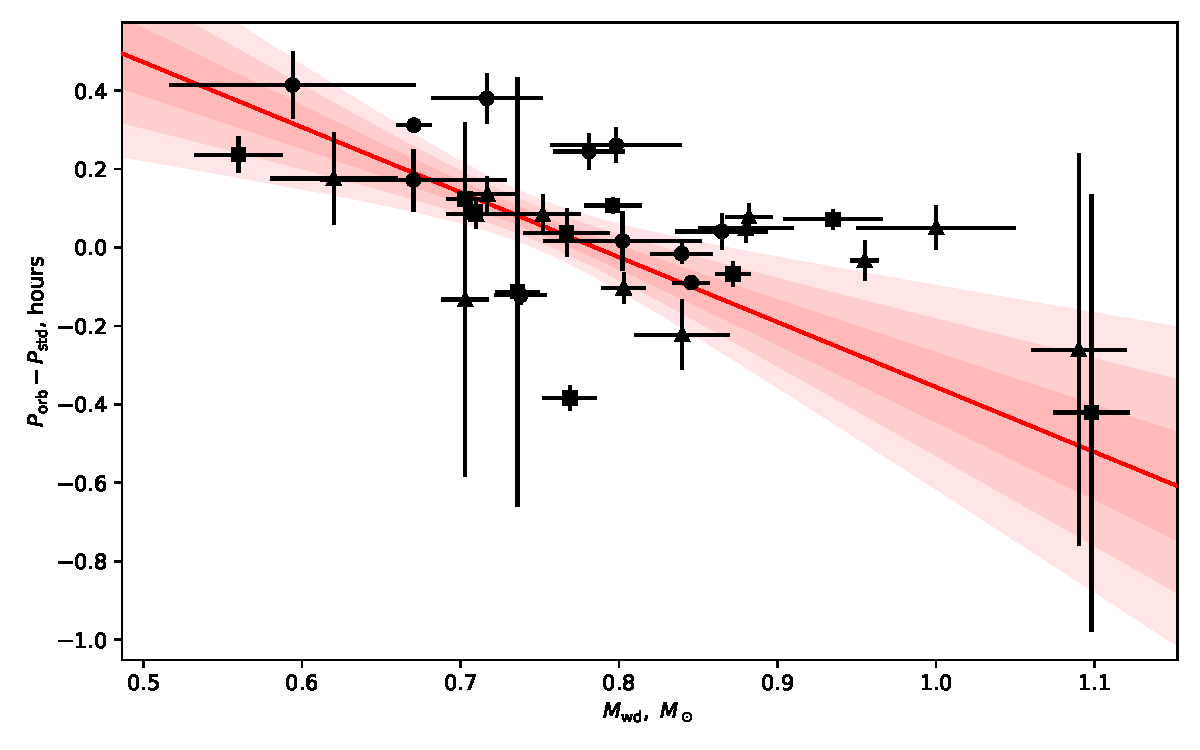
\includegraphics[width=\columnwidth]{figures/results/Mdot/Period_excess_Mwd.pdf}
    \caption{The relation between the two body masses, and the period excess, $P_{\rm ex}$ is shown. The observed data are keyed the same as Figure~\ref{fig:12 new cvs:donor model with eclipsers plotted}, and the {\bf solid red line} shows the best-fit solution to the data. {\bf Shaded red regions} show successively lower confidence intervals of the fit, with the darkest region being $1\sigma$ confidence, and the lightest region being $3\sigma$ confidence. The lines of best fit have the forms: $P_{\rm ex} = -(4.07\pm0.83) M_{\rm donor}/M_\odot + (0.32\pm0.06)$ and $P_{\rm ex} / \mathrm{hours} = -(1.62\pm0.27) M_{\rm wd}/M_\odot + (1.34\pm0.21)$.}
    \label{fig:period excess}
\end{figure}
% \begin{figure}
%     \centering
%     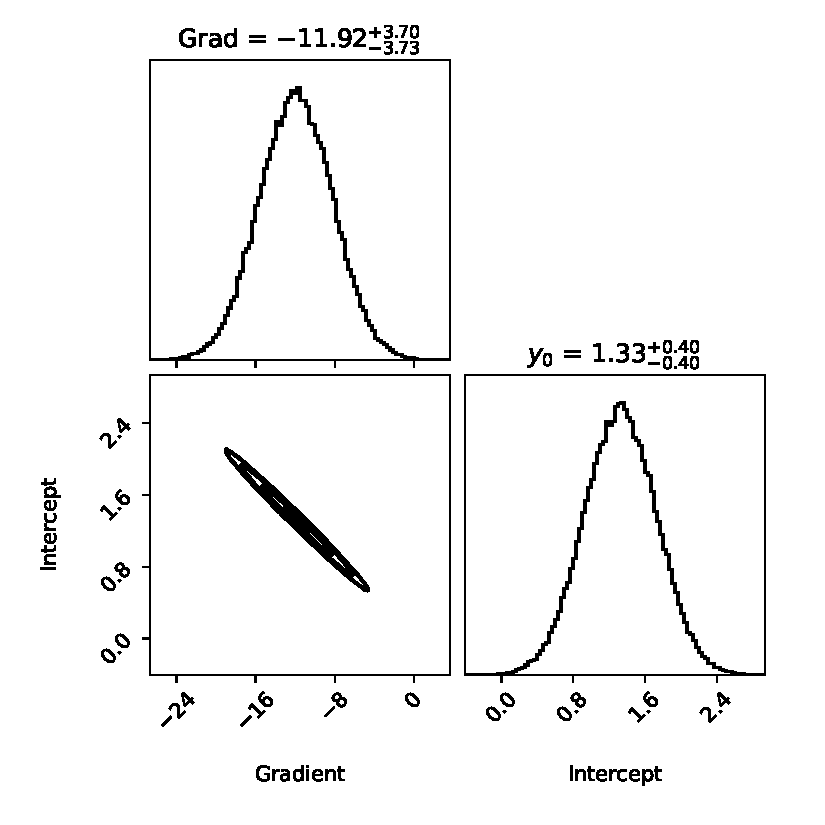
\includegraphics[width=\columnwidth]{figures/results/Mdot/Period_excess_Mr_corner.pdf}
%     \caption{Showing the distribution of the best fit to the $M_{\rm donor} - P_{\rm ex}$ relationship plotted in the top panel of Figure~\ref{fig:period excess}.}
%     \label{fig:period excess donor_corner}
% \end{figure}
% \begin{figure}
%     \centering
%     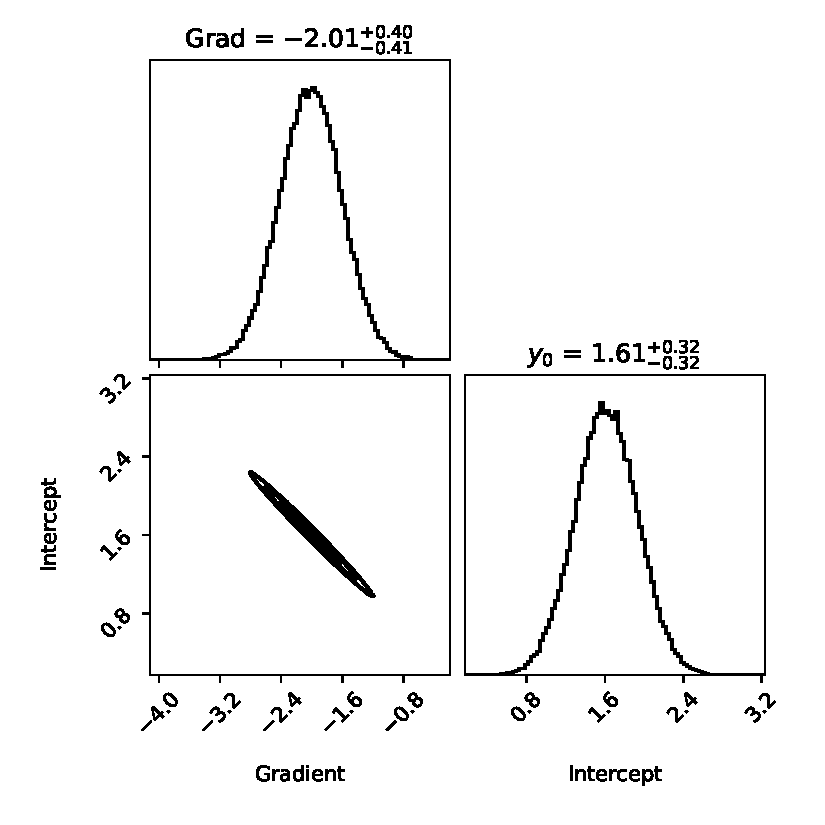
\includegraphics[width=\columnwidth]{figures/results/Mdot/Period_excess_Mwd_corner.pdf}
%     \caption{Showing the distribution of the best fit to the $M_{\rm wd} - P_{\rm ex}$ relationship plotted in the bottom panel of Figure~\ref{fig:period excess}.}
%     \label{fig:period excess white dwarf corner}
% \end{figure}


% \section{Summarising remarks}